\documentclass[twoside]{book}

% Packages required by doxygen
\usepackage{fixltx2e}
\usepackage{calc}
\usepackage{doxygen}
\usepackage[export]{adjustbox} % also loads graphicx
\usepackage{graphicx}
\usepackage[utf8]{inputenc}
\usepackage{makeidx}
\usepackage{multicol}
\usepackage{multirow}
\PassOptionsToPackage{warn}{textcomp}
\usepackage{textcomp}
\usepackage[nointegrals]{wasysym}
\usepackage[table]{xcolor}

% Font selection
\usepackage[T1]{fontenc}
\usepackage[scaled=.90]{helvet}
\usepackage{courier}
\usepackage{amssymb}
\usepackage{sectsty}
\renewcommand{\familydefault}{\sfdefault}
\allsectionsfont{%
  \fontseries{bc}\selectfont%
  \color{darkgray}%
}
\renewcommand{\DoxyLabelFont}{%
  \fontseries{bc}\selectfont%
  \color{darkgray}%
}
\newcommand{\+}{\discretionary{\mbox{\scriptsize$\hookleftarrow$}}{}{}}

% Page & text layout
\usepackage{geometry}
\geometry{%
  a4paper,%
  top=2.5cm,%
  bottom=2.5cm,%
  left=2.5cm,%
  right=2.5cm%
}
\tolerance=750
\hfuzz=15pt
\hbadness=750
\setlength{\emergencystretch}{15pt}
\setlength{\parindent}{0cm}
\setlength{\parskip}{3ex plus 2ex minus 2ex}
\makeatletter
\renewcommand{\paragraph}{%
  \@startsection{paragraph}{4}{0ex}{-1.0ex}{1.0ex}{%
    \normalfont\normalsize\bfseries\SS@parafont%
  }%
}
\renewcommand{\subparagraph}{%
  \@startsection{subparagraph}{5}{0ex}{-1.0ex}{1.0ex}{%
    \normalfont\normalsize\bfseries\SS@subparafont%
  }%
}
\makeatother

% Headers & footers
\usepackage{fancyhdr}
\pagestyle{fancyplain}
\fancyhead[LE]{\fancyplain{}{\bfseries\thepage}}
\fancyhead[CE]{\fancyplain{}{}}
\fancyhead[RE]{\fancyplain{}{\bfseries\leftmark}}
\fancyhead[LO]{\fancyplain{}{\bfseries\rightmark}}
\fancyhead[CO]{\fancyplain{}{}}
\fancyhead[RO]{\fancyplain{}{\bfseries\thepage}}
\fancyfoot[LE]{\fancyplain{}{}}
\fancyfoot[CE]{\fancyplain{}{}}
\fancyfoot[RE]{\fancyplain{}{\bfseries\scriptsize Generated by Doxygen }}
\fancyfoot[LO]{\fancyplain{}{\bfseries\scriptsize Generated by Doxygen }}
\fancyfoot[CO]{\fancyplain{}{}}
\fancyfoot[RO]{\fancyplain{}{}}
\renewcommand{\footrulewidth}{0.4pt}
\renewcommand{\chaptermark}[1]{%
  \markboth{#1}{}%
}
\renewcommand{\sectionmark}[1]{%
  \markright{\thesection\ #1}%
}

% Indices & bibliography
\usepackage{natbib}
\usepackage[titles]{tocloft}
\setcounter{tocdepth}{3}
\setcounter{secnumdepth}{5}
\makeindex

% Custom commands
\newcommand{\clearemptydoublepage}{%
  \newpage{\pagestyle{empty}\cleardoublepage}%
}

\usepackage{caption}
\captionsetup{labelsep=space,justification=centering,font={bf},singlelinecheck=off,skip=4pt,position=top}

%===== C O N T E N T S =====

\begin{document}

% Titlepage & ToC
\pagenumbering{alph}
\begin{titlepage}
\vspace*{7cm}
\begin{center}%
{\Large Lo\+Ra\+W\+AN }\\
\vspace*{1cm}
{\large Generated by Doxygen 1.8.13}\\
\end{center}
\end{titlepage}
\clearemptydoublepage
\pagenumbering{roman}
\tableofcontents
\clearemptydoublepage
\pagenumbering{arabic}

%--- Begin generated contents ---
\chapter{Host server for Lora server cluster.}
\label{md__r_e_a_d_m_e}
Hosts all the servers and provides common scripts used among all the hosted servers. Main.\+php found in this folder is used to start the hosted servers by running it and giving it a server name as the first argument. Hosted servers may define additional arguments.

Current list of hosted servers and their names are as followed.
\begin{DoxyItemize}
\item M\+Q\+TT server, mqtt
\item RT server, rt
\item C\+AC server, cac
\end{DoxyItemize}

Here are short descriptions of each listed servers. More detailed information can be found from their own readmes. M\+Q\+TT M\+Q\+TT server is responsible for receiving data from The Things Network backend, to which the all the sensor nodes send their data. M\+Q\+TT server is capable of storing and forwarding the received data. The data is forwarded to the realtime server using sockets.

RT RT server is a realtime server managing all the realtime client connections to the webserver. It also takes care of catering the clients with data they are interested in. The data is received from the M\+Q\+TT server through sockets.

C\+AC C\+AC is a command \& control server used to manage and test the server cluster. For now it is only capable of sending messages to RT server due to M\+Q\+TT server being a bit challenging to make play nice in this kind of manner due to its architecture. It is possible to send fake data all the way to the browser clients for testing purposes. Sending control commands is also possible. So far the only supported command is terminate. More commands for administration and testing can be easily added one the architecture gets more consistent. 
\chapter{Command \& Control server}
\label{md_servers_cacserver__r_e_a_d_m_e}
This is a c\&c -\/server for \doxyref{Lora}{p.}{namespace_lora} cluster, hosted under the main server. Although, server might be a misleading name for this tool since it does not really serve anything. It is more like an interface to allow testing and administration of other hosted servers. Must be started with the main server\textquotesingle{}s main.\+php with cac as its first argument. 
\chapter{ap-\/lorawan-\/iot-\/mqttserver}
\label{md_servers_mqttserver__r_e_a_d_m_e}
This is an M\+Q\+TT server for fetching sensor data from a The Things Network -\/backend.

Must be started using host server\textquotesingle{}s main.\+php to make the autoloader work. Server name required for start up is mqtt. 
\chapter{ap-\/lorawan-\/iot-\/server}
\label{md_servers_webserver__r_e_a_d_m_e}
\input{md_servers_webserver__r_e_a_d_m_e}
\chapter{Todo List}
\label{todo}

\begin{DoxyRefList}
\item[\label{todo__todo000001}%
Class \doxyref{Configuration}{p.}{class_lora_1_1_configuration} ]Start using \$paths and \$exts.  
\item[\label{todo__todo000007}%
Global \doxyref{Control\+Server\+:\+:broadcast}{p.}{class_lora_1_1_control_server_ab671527a81a457e51152cc532c716faa} (string \$command)]Write message subscription system.  
\item[\label{todo__todo000006}%
Global \doxyref{Data\+Server\+:\+:broadcast}{p.}{class_lora_1_1_data_server_a883eaf25eb21a0ba827bb9a9a3593861} (array \$msg, array \&\$messages)]Internal message processing (terminate). Broadcasts a received message to other server systems. Only interested one at the moment is the realtime sever which in turn broadcasts it onwards to clients who are interested in it.  
\item[\label{todo__todo000002}%
Class \doxyref{D\+B\+Connection}{p.}{class_d_b_connection} ]Move database access credentials to external file.  
\item[\label{todo__todo000003}%
Global \doxyref{D\+B\+Connection\+:\+:connect}{p.}{class_d_b_connection_a1191ef26fe6381a3bfbd33c0c6f7b9f4} (array \&\$db)]Automatize database type fetching so that this switch statement does not require updating everytime a new database type is added.  
\item[\label{todo__todo000014}%
Class \doxyref{Html\+Tag}{p.}{class_html_1_1_html_tag} ]Needs improvements and has to better comply H\+T\+ML structure.
\begin{DoxyItemize}
\item Add an array for inner contents.
\item Add utility funtions for certain commonly used attributes such as id and class.
\item A better approach to creating an H\+T\+ML management system would be to write specialized attribute classes instead of tag classes.  
\end{DoxyItemize}
\item[\label{todo__todo000009}%
Global \doxyref{Page\+:\+:finalize}{p.}{class_lora_1_1_page_a9caaa1f5ea6177e55f13ebe7dec2bd60} ()]Should be relocated. A possible place would be \doxyref{Page\+Manager}{p.}{class_lora_1_1_page_manager}.  
\item[\label{todo__todo000008}%
Global \doxyref{Page\+:\+:load\+View}{p.}{class_lora_1_1_page_a943f0df56a6f8dbc260ddb31925ce4f6} (string \$view)]Rename to load. Loads a \doxyref{Page}{p.}{class_lora_1_1_page}  
\item[\label{todo__todo000010}%
Global \doxyref{Page\+:\+:parse\+Views}{p.}{class_lora_1_1_page_a49b28f2ca7604e14af0d5829b4e8cc4a} (array \$views)]Needs cleaning  
\item[\label{todo__todo000011}%
Global \doxyref{Page\+View\+:\+:id}{p.}{class_lora_1_1_page_view_a087060b582403885d08e89ad894ecc5d} ()]This method should be renamed to \textquotesingle{}name\textquotesingle{}.  
\item[\label{todo__todo000004}%
Class \doxyref{Request\+Data}{p.}{class_request_data} ]Write type checks for default values and resolve to null if they are of incorrect type.  
\item[\label{todo__todo000012}%
Global \doxyref{Request\+Handler\+:\+:handle\+Api\+Request}{p.}{class_lora_1_1_request_handler_af59b79c7f32e254704d9388105a67bee} (array \$action)]Possibly add support to return X\+ML responses.  
\item[\label{todo__todo000013}%
Global \doxyref{Request\+Handler\+:\+:resolve\+Call}{p.}{class_lora_1_1_request_handler_a6fc4ced934cdeb3ef1d5a207ffb2a1e1} (array \$action, string \$file\+Path, string \$file\+Type, string \$namespace)]Move page processing somewhere else. 
\end{DoxyRefList}
\chapter{Namespace Index}
\section{Namespace List}
Here is a list of all documented namespaces with brief descriptions\+:\begin{DoxyCompactList}
\item\contentsline{section}{\hyperlink{namespace_html}{Html} }{\pageref{namespace_html}}{}
\item\contentsline{section}{\hyperlink{namespace_lora}{Lora} }{\pageref{namespace_lora}}{}
\item\contentsline{section}{\hyperlink{namespace_lora_1_1_api}{Lora\textbackslash{}\+Api} }{\pageref{namespace_lora_1_1_api}}{}
\item\contentsline{section}{\hyperlink{namespace_lora_1_1_content}{Lora\textbackslash{}\+Content} }{\pageref{namespace_lora_1_1_content}}{}
\item\contentsline{section}{\hyperlink{namespace_lora_1_1_server}{Lora\textbackslash{}\+Server} }{\pageref{namespace_lora_1_1_server}}{}
\end{DoxyCompactList}

\chapter{Hierarchical Index}
\section{Class Hierarchy}
This inheritance list is sorted roughly, but not completely, alphabetically\+:\begin{DoxyCompactList}
\item \contentsline{section}{Base\+Action}{\pageref{class_lora_1_1_base_action}}{}
\begin{DoxyCompactList}
\item \contentsline{section}{Action\+\_\+\+Data}{\pageref{class_lora_1_1_api_1_1_action___data}}{}
\item \contentsline{section}{Action\+\_\+\+Device}{\pageref{class_lora_1_1_api_1_1_action___device}}{}
\item \contentsline{section}{Action\+\_\+\+Socket}{\pageref{class_lora_1_1_api_1_1_action___socket}}{}
\item \contentsline{section}{Action\+\_\+\+Test}{\pageref{class_lora_1_1_api_1_1_action___test}}{}
\item \contentsline{section}{Content\+\_\+\+Asd}{\pageref{class_lora_1_1_content_1_1_content___asd}}{}
\item \contentsline{section}{Content\+\_\+\+Device}{\pageref{class_lora_1_1_content_1_1_content___device}}{}
\item \contentsline{section}{Content\+\_\+\+Devices}{\pageref{class_lora_1_1_content_1_1_content___devices}}{}
\item \contentsline{section}{Content\+\_\+\+Home}{\pageref{class_lora_1_1_content_1_1_content___home}}{}
\item \contentsline{section}{Content\+\_\+\+Info}{\pageref{class_lora_1_1_content_1_1_content___info}}{}
\item \contentsline{section}{Content\+\_\+\+Rtfeed}{\pageref{class_lora_1_1_content_1_1_content___rtfeed}}{}
\end{DoxyCompactList}
\item \contentsline{section}{Command}{\pageref{class_lora_1_1_server_1_1_command}}{}
\item \contentsline{section}{Config}{\pageref{class_lora_1_1_config}}{}
\item \contentsline{section}{Configuration}{\pageref{class_lora_1_1_configuration}}{}
\item \contentsline{section}{D\+AO}{\pageref{class_d_a_o}}{}
\item \contentsline{section}{Data\+Lib}{\pageref{class_data_lib}}{}
\item \contentsline{section}{Data\+Server}{\pageref{class_data_server}}{}
\item \contentsline{section}{D\+B\+Connection}{\pageref{class_d_b_connection}}{}
\item \contentsline{section}{Html\+Lib}{\pageref{class_html_1_1_html_lib}}{}
\item \contentsline{section}{Html\+Tag}{\pageref{class_html_1_1_html_tag}}{}
\begin{DoxyCompactList}
\item \contentsline{section}{Link}{\pageref{class_html_1_1_link}}{}
\end{DoxyCompactList}
\item \contentsline{section}{Internal\+M\+SG}{\pageref{class_internal_m_s_g}}{}
\item \contentsline{section}{Lib}{\pageref{class_lib}}{}
\item \contentsline{section}{Messenger}{\pageref{class_lora_1_1_messenger}}{}
\item \contentsline{section}{Page}{\pageref{class_lora_1_1_page}}{}
\item \contentsline{section}{Page\+Component}{\pageref{class_lora_1_1_page_component}}{}
\item \contentsline{section}{Page\+Manager}{\pageref{class_lora_1_1_page_manager}}{}
\item \contentsline{section}{Page\+View}{\pageref{class_lora_1_1_page_view}}{}
\item \contentsline{section}{Request\+Data}{\pageref{class_request_data}}{}
\item \contentsline{section}{Request\+Handler}{\pageref{class_lora_1_1_request_handler}}{}
\item \contentsline{section}{Response\+Crafter}{\pageref{class_lora_1_1_response_crafter}}{}
\item \contentsline{section}{User}{\pageref{class_lora_1_1_user}}{}
\item Web\+Socket\+Server\begin{DoxyCompactList}
\item \contentsline{section}{Control\+Server}{\pageref{class_control_server}}{}
\item \contentsline{section}{echo\+Server}{\pageref{classecho_server}}{}
\item \contentsline{section}{Control\+Server}{\pageref{class_lora_1_1_api_1_1_control_server}}{}
\item \contentsline{section}{echo\+Server}{\pageref{class_lora_1_1_api_1_1echo_server}}{}
\end{DoxyCompactList}
\end{DoxyCompactList}

\chapter{Data Structure Index}
\section{Data Structures}
Here are the data structures with brief descriptions\+:\begin{DoxyCompactList}
\item\contentsline{section}{\hyperlink{class_lora_1_1_api_1_1_action___data}{Action\+\_\+\+Data} }{\pageref{class_lora_1_1_api_1_1_action___data}}{}
\item\contentsline{section}{\hyperlink{class_lora_1_1_api_1_1_action___device}{Action\+\_\+\+Device} }{\pageref{class_lora_1_1_api_1_1_action___device}}{}
\item\contentsline{section}{\hyperlink{class_lora_1_1_api_1_1_action___socket}{Action\+\_\+\+Socket} }{\pageref{class_lora_1_1_api_1_1_action___socket}}{}
\item\contentsline{section}{\hyperlink{class_lora_1_1_api_1_1_action___test}{Action\+\_\+\+Test} }{\pageref{class_lora_1_1_api_1_1_action___test}}{}
\item\contentsline{section}{\hyperlink{class_lora_1_1_base_action}{Base\+Action} }{\pageref{class_lora_1_1_base_action}}{}
\item\contentsline{section}{\hyperlink{class_lora_1_1_server_1_1_command}{Command} }{\pageref{class_lora_1_1_server_1_1_command}}{}
\item\contentsline{section}{\hyperlink{class_lora_1_1_config}{Config} }{\pageref{class_lora_1_1_config}}{}
\item\contentsline{section}{\hyperlink{class_lora_1_1_configuration}{Configuration} }{\pageref{class_lora_1_1_configuration}}{}
\item\contentsline{section}{\hyperlink{class_lora_1_1_content_1_1_content___asd}{Content\+\_\+\+Asd} }{\pageref{class_lora_1_1_content_1_1_content___asd}}{}
\item\contentsline{section}{\hyperlink{class_lora_1_1_content_1_1_content___device}{Content\+\_\+\+Device} }{\pageref{class_lora_1_1_content_1_1_content___device}}{}
\item\contentsline{section}{\hyperlink{class_lora_1_1_content_1_1_content___devices}{Content\+\_\+\+Devices} }{\pageref{class_lora_1_1_content_1_1_content___devices}}{}
\item\contentsline{section}{\hyperlink{class_lora_1_1_content_1_1_content___home}{Content\+\_\+\+Home} }{\pageref{class_lora_1_1_content_1_1_content___home}}{}
\item\contentsline{section}{\hyperlink{class_lora_1_1_content_1_1_content___info}{Content\+\_\+\+Info} }{\pageref{class_lora_1_1_content_1_1_content___info}}{}
\item\contentsline{section}{\hyperlink{class_lora_1_1_content_1_1_content___rtfeed}{Content\+\_\+\+Rtfeed} }{\pageref{class_lora_1_1_content_1_1_content___rtfeed}}{}
\item\contentsline{section}{\hyperlink{class_lora_1_1_api_1_1_control_server}{Control\+Server} }{\pageref{class_lora_1_1_api_1_1_control_server}}{}
\item\contentsline{section}{\hyperlink{class_control_server}{Control\+Server} }{\pageref{class_control_server}}{}
\item\contentsline{section}{\hyperlink{class_d_a_o}{D\+AO} }{\pageref{class_d_a_o}}{}
\item\contentsline{section}{\hyperlink{class_data_lib}{Data\+Lib} }{\pageref{class_data_lib}}{}
\item\contentsline{section}{\hyperlink{class_data_server}{Data\+Server} }{\pageref{class_data_server}}{}
\item\contentsline{section}{\hyperlink{class_d_b_connection}{D\+B\+Connection} }{\pageref{class_d_b_connection}}{}
\item\contentsline{section}{\hyperlink{class_lora_1_1_api_1_1echo_server}{echo\+Server} }{\pageref{class_lora_1_1_api_1_1echo_server}}{}
\item\contentsline{section}{\hyperlink{classecho_server}{echo\+Server} }{\pageref{classecho_server}}{}
\item\contentsline{section}{\hyperlink{class_html_1_1_html_lib}{Html\+Lib} }{\pageref{class_html_1_1_html_lib}}{}
\item\contentsline{section}{\hyperlink{class_html_1_1_html_tag}{Html\+Tag} }{\pageref{class_html_1_1_html_tag}}{}
\item\contentsline{section}{\hyperlink{class_internal_m_s_g}{Internal\+M\+SG} }{\pageref{class_internal_m_s_g}}{}
\item\contentsline{section}{\hyperlink{class_lib}{Lib} }{\pageref{class_lib}}{}
\item\contentsline{section}{\hyperlink{class_html_1_1_link}{Link} }{\pageref{class_html_1_1_link}}{}
\item\contentsline{section}{\hyperlink{class_lora_1_1_messenger}{Messenger} }{\pageref{class_lora_1_1_messenger}}{}
\item\contentsline{section}{\hyperlink{class_lora_1_1_page}{Page} }{\pageref{class_lora_1_1_page}}{}
\item\contentsline{section}{\hyperlink{class_lora_1_1_page_component}{Page\+Component} }{\pageref{class_lora_1_1_page_component}}{}
\item\contentsline{section}{\hyperlink{class_lora_1_1_page_manager}{Page\+Manager} }{\pageref{class_lora_1_1_page_manager}}{}
\item\contentsline{section}{\hyperlink{class_lora_1_1_page_view}{Page\+View} }{\pageref{class_lora_1_1_page_view}}{}
\item\contentsline{section}{\hyperlink{class_request_data}{Request\+Data} }{\pageref{class_request_data}}{}
\item\contentsline{section}{\hyperlink{class_lora_1_1_request_handler}{Request\+Handler} }{\pageref{class_lora_1_1_request_handler}}{}
\item\contentsline{section}{\hyperlink{class_lora_1_1_response_crafter}{Response\+Crafter} }{\pageref{class_lora_1_1_response_crafter}}{}
\item\contentsline{section}{\hyperlink{class_lora_1_1_user}{User} }{\pageref{class_lora_1_1_user}}{}
\end{DoxyCompactList}

\chapter{Namespace Documentation}
\section{Html Namespace Reference}
\label{namespace_html}\index{Html@{Html}}
\subsection*{Data Structures}
\begin{DoxyCompactItemize}
\item 
class \textbf{ Html\+Lib}
\item 
class \textbf{ Html\+Tag}
\item 
class \textbf{ Link}
\end{DoxyCompactItemize}


\subsection{Detailed Description}
Namespace containing H\+T\+ML related classes and functionality. Mostly used together with Twig to create a powerful H\+T\+ML generating pipeline which covers some of Twigs weaknesses by utilizing H\+T\+ML tag classes which allow printing highly complex tags with ease withing Twig templates. 
\section{Lora Namespace Reference}
\label{namespace_lora}\index{Lora@{Lora}}
\subsection*{Namespaces}
\begin{DoxyCompactItemize}
\item 
 \textbf{ Api}
\item 
 \textbf{ Content}
\item 
 \textbf{ Server}
\end{DoxyCompactItemize}
\subsection*{Data Structures}
\begin{DoxyCompactItemize}
\item 
class \textbf{ Base\+Action}
\item 
class \textbf{ Config}
\item 
class \textbf{ Configuration}
\item 
class \textbf{ Control\+Server}
\item 
class \textbf{ D\+AO}
\item 
class \textbf{ Data\+Server}
\item 
class \textbf{ Messenger}
\item 
class \textbf{ Page}
\item 
class \textbf{ Page\+Component}
\item 
class \textbf{ Page\+Manager}
\item 
class \textbf{ Page\+View}
\item 
class \textbf{ Realtime\+Server}
\item 
class \textbf{ Request\+Handler}
\item 
class \textbf{ Response\+Crafter}
\item 
class \textbf{ User}
\end{DoxyCompactItemize}
\subsection*{Functions}
\begin{DoxyCompactItemize}
\item 
\textbf{ login} ()
\item 
\textbf{ logout} ()
\item 
\textbf{ is\+Logged\+In} (\$session=null)
\item 
\textbf{ allow\+Access} ()
\item 
\textbf{ get\+User} ()
\end{DoxyCompactItemize}


\subsection{Detailed Description}
Main namespace for this system. Hosts all other namespaces and backbone scripts for hosted servers. 

\subsection{Function Documentation}
\mbox{\label{namespace_lora_a94879a930ed3b8684851ff98e9220a27}} 
\index{Lora@{Lora}!allow\+Access@{allow\+Access}}
\index{allow\+Access@{allow\+Access}!Lora@{Lora}}
\subsubsection{allow\+Access()}
{\footnotesize\ttfamily Lora\textbackslash{}allow\+Access (\begin{DoxyParamCaption}{ }\end{DoxyParamCaption})}

A function to determine whether or not the user should be allowed to access requested content.  Should take user information as parameter. 
\begin{DoxyCode}
37                         \{
38     \textcolor{keywordflow}{return} \textcolor{keyword}{true};
39 \}
\end{DoxyCode}
\mbox{\label{namespace_lora_a881d230aaa8a5510d5c80f0ed1497129}} 
\index{Lora@{Lora}!get\+User@{get\+User}}
\index{get\+User@{get\+User}!Lora@{Lora}}
\subsubsection{get\+User()}
{\footnotesize\ttfamily Lora\textbackslash{}get\+User (\begin{DoxyParamCaption}{ }\end{DoxyParamCaption})}

A function to return current user object performing the request. \begin{DoxyReturn}{Returns}
An instance of user. 
\end{DoxyReturn}

\begin{DoxyCode}
45                     \{
46     \textcolor{keywordflow}{return} User::Dummy ();
47 \}
\end{DoxyCode}
Here is the caller graph for this function\+:\nopagebreak
\begin{figure}[H]
\begin{center}
\leavevmode
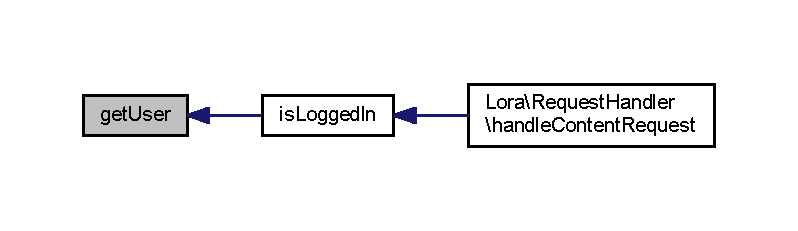
\includegraphics[width=350pt]{namespace_lora_a881d230aaa8a5510d5c80f0ed1497129_icgraph}
\end{center}
\end{figure}
\mbox{\label{namespace_lora_a538956ba5c1427dd64c41ea1cdc5bddb}} 
\index{Lora@{Lora}!is\+Logged\+In@{is\+Logged\+In}}
\index{is\+Logged\+In@{is\+Logged\+In}!Lora@{Lora}}
\subsubsection{is\+Logged\+In()}
{\footnotesize\ttfamily Lora\textbackslash{}is\+Logged\+In (\begin{DoxyParamCaption}\item[{}]{\$session = {\ttfamily null} }\end{DoxyParamCaption})}

A function for checking whether or not the user has an active session. 
\begin{DoxyCode}
28                                       \{ # Should take session information as parameter.
29     getUser ();
30     \textcolor{keywordflow}{return} \textcolor{keyword}{true};
31 \}
\end{DoxyCode}
Here is the call graph for this function\+:\nopagebreak
\begin{figure}[H]
\begin{center}
\leavevmode
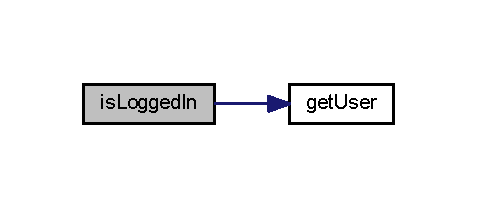
\includegraphics[width=229pt]{namespace_lora_a538956ba5c1427dd64c41ea1cdc5bddb_cgraph}
\end{center}
\end{figure}
Here is the caller graph for this function\+:\nopagebreak
\begin{figure}[H]
\begin{center}
\leavevmode
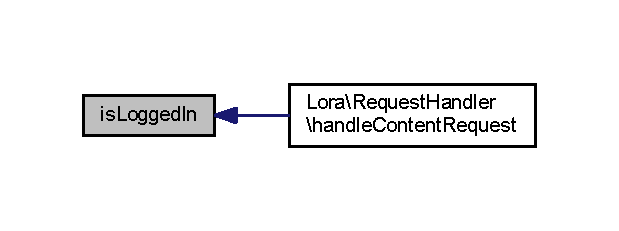
\includegraphics[width=297pt]{namespace_lora_a538956ba5c1427dd64c41ea1cdc5bddb_icgraph}
\end{center}
\end{figure}
\mbox{\label{namespace_lora_a6334cdbb86812dbd18f093463e7c3023}} 
\index{Lora@{Lora}!login@{login}}
\index{login@{login}!Lora@{Lora}}
\subsubsection{login()}
{\footnotesize\ttfamily Lora\textbackslash{}login (\begin{DoxyParamCaption}{ }\end{DoxyParamCaption})}

N\+O\+TE\+: Replace the contents of these functions with actual session management logic in order to restrict system access.

Some changes to \doxyref{Request\+Handler}{p.}{class_lora_1_1_request_handler} may be required in order to make these functions work in a fluid manner. A function to contain login routine. 
\begin{DoxyCode}
15                   \{
16     \textcolor{keywordflow}{return} \textcolor{keyword}{true};
17 \}
\end{DoxyCode}
Here is the caller graph for this function\+:\nopagebreak
\begin{figure}[H]
\begin{center}
\leavevmode
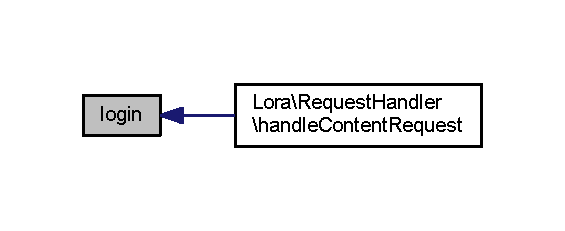
\includegraphics[width=271pt]{namespace_lora_a6334cdbb86812dbd18f093463e7c3023_icgraph}
\end{center}
\end{figure}
\mbox{\label{namespace_lora_a801b7854cd8f787f174a6b501bf517bb}} 
\index{Lora@{Lora}!logout@{logout}}
\index{logout@{logout}!Lora@{Lora}}
\subsubsection{logout()}
{\footnotesize\ttfamily Lora\textbackslash{}logout (\begin{DoxyParamCaption}{ }\end{DoxyParamCaption})}

A function to contain logout routine. 
\begin{DoxyCode}
22                    \{
23 \}
\end{DoxyCode}

\section{Lora\textbackslash{}Api Namespace Reference}
\label{namespace_lora_1_1_api}\index{Lora\textbackslash{}\+Api@{Lora\textbackslash{}\+Api}}
\subsection*{Data Structures}
\begin{DoxyCompactItemize}
\item 
class \textbf{ Action\+\_\+\+Data}
\item 
class \textbf{ Action\+\_\+\+Device}
\item 
class \textbf{ Action\+\_\+\+Socket}
\item 
class \textbf{ Action\+\_\+\+Test}
\item 
class \textbf{ Control\+Server}
\item 
class \textbf{ echo\+Server}
\end{DoxyCompactItemize}
\subsection*{Variables}
\begin{DoxyCompactItemize}
\item 
\mbox{\label{namespace_lora_1_1_api_a76dbdd763137ce9b516dc94d3a16fe60}} 
{\bfseries \$echo} = new \textbf{ echo\+Server} (\char`\"{}0.\+0.\+0.\+0\char`\"{}, \char`\"{}9000\char`\"{})
\item 
\mbox{\label{namespace_lora_1_1_api_ab515c178ff35f1107f2bc2198e4dee4b}} 
{\bfseries \$inter} = new \textbf{ Control\+Server} (\$echo, \char`\"{}127.\+0.\+0.\+1\char`\"{}, \char`\"{}9001\char`\"{})
\end{DoxyCompactItemize}


\subsection{Detailed Description}
Namespace for hosting this systems web A\+PI and all related scripts. 
\hypertarget{namespace_lora_1_1_content}{}\section{Lora\textbackslash{}Content Namespace Reference}
\label{namespace_lora_1_1_content}\index{Lora\textbackslash{}\+Content@{Lora\textbackslash{}\+Content}}
\subsection*{Data Structures}
\begin{DoxyCompactItemize}
\item 
class \hyperlink{class_lora_1_1_content_1_1_content___asd}{Content\+\_\+\+Asd}
\item 
class \hyperlink{class_lora_1_1_content_1_1_content___device}{Content\+\_\+\+Device}
\item 
class \hyperlink{class_lora_1_1_content_1_1_content___devices}{Content\+\_\+\+Devices}
\item 
class \hyperlink{class_lora_1_1_content_1_1_content___home}{Content\+\_\+\+Home}
\item 
class \hyperlink{class_lora_1_1_content_1_1_content___info}{Content\+\_\+\+Info}
\item 
class \hyperlink{class_lora_1_1_content_1_1_content___rtfeed}{Content\+\_\+\+Rtfeed}
\end{DoxyCompactItemize}


\subsection{Detailed Description}
Namespace for hosting all content related functionality of this system. This includes all web page creation and management scripts. 
\section{Lora\textbackslash{}Server Namespace Reference}
\label{namespace_lora_1_1_server}\index{Lora\textbackslash{}\+Server@{Lora\textbackslash{}\+Server}}
\subsection*{Data Structures}
\begin{DoxyCompactItemize}
\item 
class \textbf{ Command}
\item 
class \textbf{ Response}
\end{DoxyCompactItemize}


\subsection{Detailed Description}
Namespace for the higher level components of this system which can not be deployed outside this system without heavy modifications. Such systems include the internal messaging subsystem, a 
\chapter{Data Structure Documentation}
\hypertarget{class_lora_1_1_api_1_1_action___data}{}\section{Action\+\_\+\+Data Class Reference}
\label{class_lora_1_1_api_1_1_action___data}\index{Action\+\_\+\+Data@{Action\+\_\+\+Data}}


Inheritance diagram for Action\+\_\+\+Data\+:
% FIG 0


Collaboration diagram for Action\+\_\+\+Data\+:
% FIG 1
\subsection*{Public Member Functions}
\begin{DoxyCompactItemize}
\item 
\mbox{\Hypertarget{class_lora_1_1_api_1_1_action___data_a3ad4bf1b146a3180b34d1327ff2abf69}\label{class_lora_1_1_api_1_1_action___data_a3ad4bf1b146a3180b34d1327ff2abf69}} 
{\bfseries \+\_\+get} (\hyperlink{class_request_data}{Request\+Data} \$req)
\item 
\mbox{\Hypertarget{class_lora_1_1_api_1_1_action___data_a50751d47a139282d1c3b08cab1b6562e}\label{class_lora_1_1_api_1_1_action___data_a50751d47a139282d1c3b08cab1b6562e}} 
{\bfseries \+\_\+post} (\hyperlink{class_request_data}{Request\+Data} \$req)
\item 
\mbox{\Hypertarget{class_lora_1_1_api_1_1_action___data_a2affcc8f31c13147c33450193b229194}\label{class_lora_1_1_api_1_1_action___data_a2affcc8f31c13147c33450193b229194}} 
{\bfseries \+\_\+put} (\hyperlink{class_request_data}{Request\+Data} \$req)
\item 
\mbox{\Hypertarget{class_lora_1_1_api_1_1_action___data_ab8ddc6de1e04524212f7d55893f78864}\label{class_lora_1_1_api_1_1_action___data_ab8ddc6de1e04524212f7d55893f78864}} 
{\bfseries \+\_\+delete} (\hyperlink{class_request_data}{Request\+Data} \$req)
\end{DoxyCompactItemize}
\subsection*{Private Member Functions}
\begin{DoxyCompactItemize}
\item 
\mbox{\Hypertarget{class_lora_1_1_api_1_1_action___data_adea63eb9d6f49832427cbb855c4c59ce}\label{class_lora_1_1_api_1_1_action___data_adea63eb9d6f49832427cbb855c4c59ce}} 
{\bfseries search} (\hyperlink{class_request_data}{Request\+Data} \$req)
\end{DoxyCompactItemize}
\subsection*{Additional Inherited Members}


The documentation for this class was generated from the following file\+:\begin{DoxyCompactItemize}
\item 
servers/webserver/server/api/data/data.\+php\end{DoxyCompactItemize}

\section{Action\+\_\+\+Device Class Reference}
\label{class_lora_1_1_api_1_1_action___device}\index{Action\+\_\+\+Device@{Action\+\_\+\+Device}}


Inheritance diagram for Action\+\_\+\+Device\+:\nopagebreak
\begin{figure}[H]
\begin{center}
\leavevmode
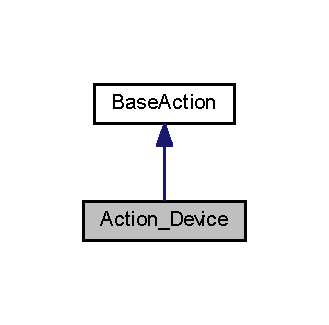
\includegraphics[width=158pt]{class_lora_1_1_api_1_1_action___device__inherit__graph}
\end{center}
\end{figure}


Collaboration diagram for Action\+\_\+\+Device\+:\nopagebreak
\begin{figure}[H]
\begin{center}
\leavevmode
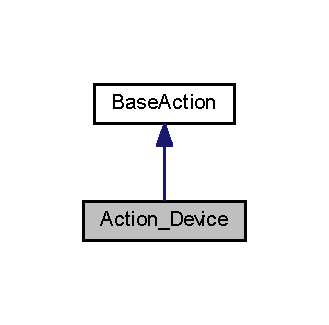
\includegraphics[width=158pt]{class_lora_1_1_api_1_1_action___device__coll__graph}
\end{center}
\end{figure}
\subsection*{Public Member Functions}
\begin{DoxyCompactItemize}
\item 
\mbox{\label{class_lora_1_1_api_1_1_action___device_a3ad4bf1b146a3180b34d1327ff2abf69}} 
{\bfseries \+\_\+get} (\textbf{ Request\+Data} \$req)
\item 
\mbox{\label{class_lora_1_1_api_1_1_action___device_a50751d47a139282d1c3b08cab1b6562e}} 
{\bfseries \+\_\+post} (\textbf{ Request\+Data} \$req)
\item 
\mbox{\label{class_lora_1_1_api_1_1_action___device_a2affcc8f31c13147c33450193b229194}} 
{\bfseries \+\_\+put} (\textbf{ Request\+Data} \$req)
\item 
\mbox{\label{class_lora_1_1_api_1_1_action___device_ab8ddc6de1e04524212f7d55893f78864}} 
{\bfseries \+\_\+delete} (\textbf{ Request\+Data} \$req)
\end{DoxyCompactItemize}
\subsection*{Private Member Functions}
\begin{DoxyCompactItemize}
\item 
\mbox{\label{class_lora_1_1_api_1_1_action___device_aaed57abc90b47df34b294e5e49ef63ae}} 
{\bfseries get\+Data} (\textbf{ Request\+Data} \$req, string \$id)
\end{DoxyCompactItemize}
\subsection*{Additional Inherited Members}


The documentation for this class was generated from the following file\+:\begin{DoxyCompactItemize}
\item 
servers/webserver/server/api/device/device.\+php\end{DoxyCompactItemize}

\section{Action\+\_\+\+Socket Class Reference}
\label{class_lora_1_1_api_1_1_action___socket}\index{Action\+\_\+\+Socket@{Action\+\_\+\+Socket}}


Inheritance diagram for Action\+\_\+\+Socket\+:\nopagebreak
\begin{figure}[H]
\begin{center}
\leavevmode
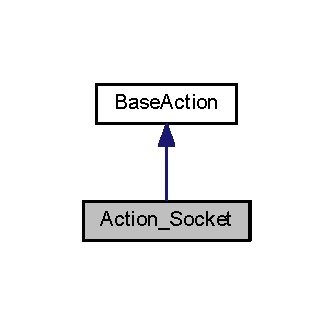
\includegraphics[width=160pt]{class_lora_1_1_api_1_1_action___socket__inherit__graph}
\end{center}
\end{figure}


Collaboration diagram for Action\+\_\+\+Socket\+:\nopagebreak
\begin{figure}[H]
\begin{center}
\leavevmode
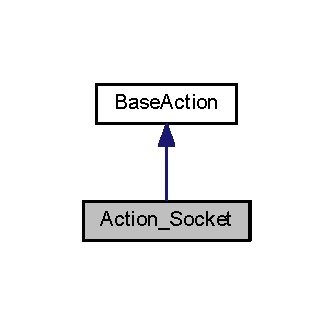
\includegraphics[width=160pt]{class_lora_1_1_api_1_1_action___socket__coll__graph}
\end{center}
\end{figure}
\subsection*{Public Member Functions}
\begin{DoxyCompactItemize}
\item 
\mbox{\label{class_lora_1_1_api_1_1_action___socket_a3ad4bf1b146a3180b34d1327ff2abf69}} 
{\bfseries \+\_\+get} (\textbf{ Request\+Data} \$req)
\item 
\mbox{\label{class_lora_1_1_api_1_1_action___socket_a50751d47a139282d1c3b08cab1b6562e}} 
{\bfseries \+\_\+post} (\textbf{ Request\+Data} \$req)
\item 
\mbox{\label{class_lora_1_1_api_1_1_action___socket_a2affcc8f31c13147c33450193b229194}} 
{\bfseries \+\_\+put} (\textbf{ Request\+Data} \$req)
\item 
\mbox{\label{class_lora_1_1_api_1_1_action___socket_ab8ddc6de1e04524212f7d55893f78864}} 
{\bfseries \+\_\+delete} (\textbf{ Request\+Data} \$req)
\end{DoxyCompactItemize}
\subsection*{Additional Inherited Members}


The documentation for this class was generated from the following file\+:\begin{DoxyCompactItemize}
\item 
servers/webserver/server/api/socket/socket.\+php\end{DoxyCompactItemize}

\section{Action\+\_\+\+Test Class Reference}
\label{class_lora_1_1_api_1_1_action___test}\index{Action\+\_\+\+Test@{Action\+\_\+\+Test}}


Inheritance diagram for Action\+\_\+\+Test\+:\nopagebreak
\begin{figure}[H]
\begin{center}
\leavevmode
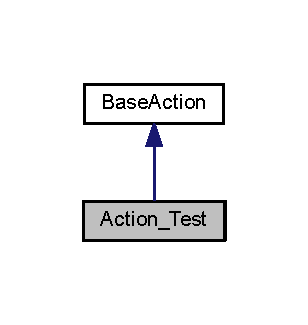
\includegraphics[width=148pt]{class_lora_1_1_api_1_1_action___test__inherit__graph}
\end{center}
\end{figure}


Collaboration diagram for Action\+\_\+\+Test\+:\nopagebreak
\begin{figure}[H]
\begin{center}
\leavevmode
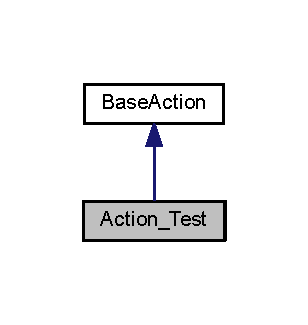
\includegraphics[width=148pt]{class_lora_1_1_api_1_1_action___test__coll__graph}
\end{center}
\end{figure}
\subsection*{Public Member Functions}
\begin{DoxyCompactItemize}
\item 
\mbox{\label{class_lora_1_1_api_1_1_action___test_a3ad4bf1b146a3180b34d1327ff2abf69}} 
{\bfseries \+\_\+get} (\textbf{ Request\+Data} \$req)
\item 
\mbox{\label{class_lora_1_1_api_1_1_action___test_a50751d47a139282d1c3b08cab1b6562e}} 
{\bfseries \+\_\+post} (\textbf{ Request\+Data} \$req)
\item 
\mbox{\label{class_lora_1_1_api_1_1_action___test_a2affcc8f31c13147c33450193b229194}} 
{\bfseries \+\_\+put} (\textbf{ Request\+Data} \$req)
\item 
\mbox{\label{class_lora_1_1_api_1_1_action___test_ab8ddc6de1e04524212f7d55893f78864}} 
{\bfseries \+\_\+delete} (\textbf{ Request\+Data} \$req)
\end{DoxyCompactItemize}
\subsection*{Additional Inherited Members}


The documentation for this class was generated from the following file\+:\begin{DoxyCompactItemize}
\item 
servers/webserver/server/api/test/test.\+php\end{DoxyCompactItemize}

\section{Base\+Action Class Reference}
\label{class_lora_1_1_base_action}\index{Base\+Action@{Base\+Action}}


Inheritance diagram for Base\+Action\+:\nopagebreak
\begin{figure}[H]
\begin{center}
\leavevmode
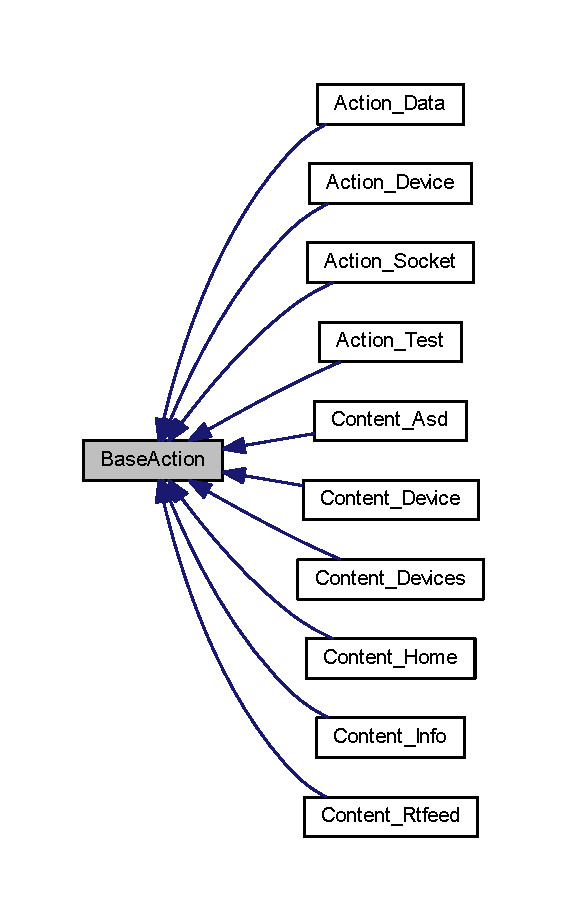
\includegraphics[width=272pt]{class_lora_1_1_base_action__inherit__graph}
\end{center}
\end{figure}
\subsection*{Public Member Functions}
\begin{DoxyCompactItemize}
\item 
\textbf{ \+\_\+\+\_\+construct} (string \$name, \textbf{ Messenger} \$mess)
\item 
\textbf{ get\+Id} ()
\item 
\textbf{ get\+Name} ()
\item 
\textbf{ run} (\textbf{ Request\+Data} \$req, string \$method, array \$excess\+Url, \textbf{ Page} \$page=null)
\end{DoxyCompactItemize}
\subsection*{Data Fields}
\begin{DoxyCompactItemize}
\item 
\mbox{\label{class_lora_1_1_base_action_a0a44e6760141442bb439b1ab1395d8ff}} 
{\bfseries \$page} = null
\item 
\mbox{\label{class_lora_1_1_base_action_ae97941710d863131c700f069b109991e}} 
{\bfseries \$id} = \textquotesingle{}\textquotesingle{}
\item 
\mbox{\label{class_lora_1_1_base_action_ab2fc40d43824ea3e1ce5d86dee0d763b}} 
{\bfseries \$name} = \textquotesingle{}\textquotesingle{}
\item 
\mbox{\label{class_lora_1_1_base_action_acf215f34a917d014776ce684a9ee8909}} 
\textbf{ \$url} = [$\,$]
\begin{DoxyCompactList}\small\item\em This should be moved to \doxyref{Request\+Data}{p.}{class_request_data} since that class was specifically created for this kind of data. \end{DoxyCompactList}\end{DoxyCompactItemize}
\subsection*{Protected Member Functions}
\begin{DoxyCompactItemize}
\item 
\textbf{ init} ()
\end{DoxyCompactItemize}
\subsection*{Protected Attributes}
\begin{DoxyCompactItemize}
\item 
\mbox{\label{class_lora_1_1_base_action_a7402b7f726abbbfe8793e75fafcd5e91}} 
{\bfseries \$mess} = null
\end{DoxyCompactItemize}


\subsection{Detailed Description}
A class from which all A\+PI and content scripts inherit. 

\subsection{Constructor \& Destructor Documentation}
\mbox{\label{class_lora_1_1_base_action_a605a9aac4f379b8beeef22a91ad9f0ff}} 
\index{Lora\+::\+Base\+Action@{Lora\+::\+Base\+Action}!\+\_\+\+\_\+construct@{\+\_\+\+\_\+construct}}
\index{\+\_\+\+\_\+construct@{\+\_\+\+\_\+construct}!Lora\+::\+Base\+Action@{Lora\+::\+Base\+Action}}
\subsubsection{\+\_\+\+\_\+construct()}
{\footnotesize\ttfamily \+\_\+\+\_\+construct (\begin{DoxyParamCaption}\item[{string}]{\$name,  }\item[{\textbf{ Messenger}}]{\$mess }\end{DoxyParamCaption})}


\begin{DoxyParams}{Parameters}
{\em \$name} & Non-\/prefixed name of this class. \\
\hline
{\em \$mess} & An instance of messenger. \\
\hline
\end{DoxyParams}

\begin{DoxyCode}
22                                                                 \{
23         $this->name             = strtolower ($name);
24         $this->mess             = $mess;
25         $this->\textcolor{keywordtype}{id}               = md5 (get\_class ($this));
26     \}
\end{DoxyCode}


\subsection{Member Function Documentation}
\mbox{\label{class_lora_1_1_base_action_a12251d0c022e9e21c137a105ff683f13}} 
\index{Lora\+::\+Base\+Action@{Lora\+::\+Base\+Action}!get\+Id@{get\+Id}}
\index{get\+Id@{get\+Id}!Lora\+::\+Base\+Action@{Lora\+::\+Base\+Action}}
\subsubsection{get\+Id()}
{\footnotesize\ttfamily get\+Id (\begin{DoxyParamCaption}{ }\end{DoxyParamCaption})}

Returns in id value of this class generated its name using md5. \begin{DoxyReturn}{Returns}
Id value unique to this action. 
\end{DoxyReturn}

\begin{DoxyCode}
32                              \{
33         \textcolor{keywordflow}{return} $this->id;
34     \}
\end{DoxyCode}
\mbox{\label{class_lora_1_1_base_action_a3d0963e68bb313b163a73f2803c64600}} 
\index{Lora\+::\+Base\+Action@{Lora\+::\+Base\+Action}!get\+Name@{get\+Name}}
\index{get\+Name@{get\+Name}!Lora\+::\+Base\+Action@{Lora\+::\+Base\+Action}}
\subsubsection{get\+Name()}
{\footnotesize\ttfamily get\+Name (\begin{DoxyParamCaption}{ }\end{DoxyParamCaption})}

In order to create an instance of this class, a shorted non-\/prefixed variation of its name must be given as parameter. This method returns that name. \begin{DoxyReturn}{Returns}
Non-\/prefixed name of this class. 
\end{DoxyReturn}

\begin{DoxyCode}
41                                \{
42         \textcolor{keywordflow}{return} $this->name;
43     \}
\end{DoxyCode}
\mbox{\label{class_lora_1_1_base_action_a4be4055f3361d4800e16bc2e2e38cda6}} 
\index{Lora\+::\+Base\+Action@{Lora\+::\+Base\+Action}!init@{init}}
\index{init@{init}!Lora\+::\+Base\+Action@{Lora\+::\+Base\+Action}}
\subsubsection{init()}
{\footnotesize\ttfamily init (\begin{DoxyParamCaption}{ }\end{DoxyParamCaption})\hspace{0.3cm}{\ttfamily [protected]}}

Overridable initialization method. Called before running H\+T\+TP method corresponding method. 
\begin{DoxyCode}
48                                : \textcolor{keywordtype}{void} \{
49     \}
\end{DoxyCode}
\mbox{\label{class_lora_1_1_base_action_af22d6f78c304d3bf1eb1f3f4716b824f}} 
\index{Lora\+::\+Base\+Action@{Lora\+::\+Base\+Action}!run@{run}}
\index{run@{run}!Lora\+::\+Base\+Action@{Lora\+::\+Base\+Action}}
\subsubsection{run()}
{\footnotesize\ttfamily run (\begin{DoxyParamCaption}\item[{\textbf{ Request\+Data}}]{\$req,  }\item[{string}]{\$method,  }\item[{array}]{\$excess\+Url,  }\item[{\textbf{ Page}}]{\$page = {\ttfamily null} }\end{DoxyParamCaption})}

Runs the action and executes an H\+T\+TP paired method. 
\begin{DoxyParams}{Parameters}
{\em \$req} & An instance of \doxyref{Request\+Data}{p.}{class_request_data} containing all the retquest parameters. \\
\hline
{\em \$method} & Converted H\+T\+TP method to be used as a method name to run the correct method. \\
\hline
{\em \$excess\+Url} & An array containing the parts of the U\+RI which were not used to resolve correct class name. \\
\hline
{\em \$page} & An optional instance of \doxyref{Page}{p.}{class_lora_1_1_page} passed only to Content\+\_\+ classes. \\
\hline
\end{DoxyParams}

\begin{DoxyCode}
58                                                                                                 : \textcolor{keywordtype}{void} \{
59         \textcolor{keywordflow}{if} (method\_exists ($this, $method)) \{
60             $this->url = $excessUrl;
61             $this->page = $page;
62             $this->init ();
63             $this->$method ($req);
64         \}
65     \}
\end{DoxyCode}


The documentation for this class was generated from the following file\+:\begin{DoxyCompactItemize}
\item 
servers/webserver/server/baseaction.\+php\end{DoxyCompactItemize}

\section{Command Class Reference}
\label{class_lora_1_1_server_1_1_command}\index{Command@{Command}}
\subsection*{Static Public Member Functions}
\begin{DoxyCompactItemize}
\item 
static \textbf{ is\+Command} (\$value)
\end{DoxyCompactItemize}
\subsection*{Data Fields}
\begin{DoxyCompactItemize}
\item 
\mbox{\label{class_lora_1_1_server_1_1_command_a51c222026c95d22d182a70dffb1274d8}} 
const \textbf{ I\+N\+V\+A\+L\+ID} = 0
\begin{DoxyCompactList}\small\item\em An invalid message. \end{DoxyCompactList}\item 
\mbox{\label{class_lora_1_1_server_1_1_command_a59322b745f918a8b5f747b08d9d5ddec}} 
const \textbf{ D\+A\+TA} = 1
\begin{DoxyCompactList}\small\item\em Data message containing data. \end{DoxyCompactList}\item 
\mbox{\label{class_lora_1_1_server_1_1_command_aff329be36615a18f3dd0bc2d393dbc2f}} 
const \textbf{ A\+C\+T\+I\+ON} = 2
\begin{DoxyCompactList}\small\item\em Action message containing a action to perform. \end{DoxyCompactList}\end{DoxyCompactItemize}


\subsection{Detailed Description}
An enum class for message types used in internal system messaging. 

\subsection{Member Function Documentation}
\mbox{\label{class_lora_1_1_server_1_1_command_a77bf97cc94921f5dc95fa09cc9d87ffe}} 
\index{Lora\+::\+Server\+::\+Command@{Lora\+::\+Server\+::\+Command}!is\+Command@{is\+Command}}
\index{is\+Command@{is\+Command}!Lora\+::\+Server\+::\+Command@{Lora\+::\+Server\+::\+Command}}
\subsubsection{is\+Command()}
{\footnotesize\ttfamily static is\+Command (\begin{DoxyParamCaption}\item[{}]{\$value }\end{DoxyParamCaption})\hspace{0.3cm}{\ttfamily [static]}}

Collects all constants in \doxyref{Command}{p.}{class_lora_1_1_server_1_1_command} during the first call and flips received array. This collection is then used to see if some value is a \doxyref{Command}{p.}{class_lora_1_1_server_1_1_command} constant or not. 
\begin{DoxyParams}{Parameters}
{\em \$value} & Value to test for constant. \\
\hline
\end{DoxyParams}
\begin{DoxyReturn}{Returns}
Returns true is \$value is a \doxyref{Command}{p.}{class_lora_1_1_server_1_1_command} value and false if not. 
\end{DoxyReturn}

\begin{DoxyCode}
20                                               \{
21         \textcolor{keyword}{static} $consts = null;
22         \textcolor{keywordflow}{if} (!$consts) \{
23             $consts = array\_flip ((\textcolor{keyword}{new} \(\backslash\)ReflectionClass (\_\_CLASS\_\_))->getConstants ());
24         \}
25         \textcolor{keywordflow}{return} isset ($consts [$value]);
26     \}
\end{DoxyCode}


The documentation for this class was generated from the following file\+:\begin{DoxyCompactItemize}
\item 
lora/command.\+php\end{DoxyCompactItemize}

\section{Config Class Reference}
\label{class_lora_1_1_config}\index{Config@{Config}}
\subsection*{Static Public Member Functions}
\begin{DoxyCompactItemize}
\item 
static \textbf{ instance} ()
\item 
static \textbf{ load\+Config} (array \$configs)
\item 
static \textbf{ get} (... \$key)
\item 
static \textbf{ path} (... \$key)
\item 
static \textbf{ paths} (... \$key)
\item 
static \textbf{ ext} (... \$key)
\item 
static \textbf{ port} (... \$key)
\item 
static \textbf{ register\+Autoloaders} ()
\item 
static \textbf{ autoloader} (\$class)
\end{DoxyCompactItemize}
\subsection*{Data Fields}
\begin{DoxyCompactItemize}
\item 
\mbox{\label{class_lora_1_1_config_a1fc0f693347c58a8714672eeffa2e134}} 
const \textbf{ P\+A\+TH} = \textquotesingle{}path\+\_\+\textquotesingle{}
\begin{DoxyCompactList}\small\item\em Path prefix which can be used in configuration files to allow them to be fetched through path method. \end{DoxyCompactList}\item 
\mbox{\label{class_lora_1_1_config_a946f0934b6d4dce0bc46dbdb9119a624}} 
const \textbf{ E\+X\+T\+E\+N\+S\+I\+ON} = \textquotesingle{}ext\+\_\+\textquotesingle{}
\begin{DoxyCompactList}\small\item\em Extension prefix which can be used in configuration files to allow them to be fetched through ext method. \end{DoxyCompactList}\item 
\mbox{\label{class_lora_1_1_config_ab9a2d2c70deaf0f75cf0ee531f6ed0b5}} 
const \textbf{ P\+O\+RT} = \textquotesingle{}port\+\_\+\textquotesingle{}
\begin{DoxyCompactList}\small\item\em Extension prefix which can be used in configuration files to allow them to be fetched through port method. \end{DoxyCompactList}\end{DoxyCompactItemize}
\subsection*{Private Attributes}
\begin{DoxyCompactItemize}
\item 
\mbox{\label{class_lora_1_1_config_a3d0d06c2ac189761041669f7fbcb6ba5}} 
{\bfseries \$configurations} = [$\,$]
\end{DoxyCompactItemize}
\subsection*{Static Private Attributes}
\begin{DoxyCompactItemize}
\item 
\mbox{\label{class_lora_1_1_config_ad9d7ce33ebb142b70e58b68052ca0ea8}} 
static {\bfseries \$instance} = null
\end{DoxyCompactItemize}


\subsection{Detailed Description}
\doxyref{Configuration}{p.}{class_lora_1_1_configuration} management class capable of managing multiple cinfiguration sets. Uses singleton pattern. Belongs to \doxyref{Lora}{p.}{namespace_lora} -\/namespace. 

\subsection{Member Function Documentation}
\mbox{\label{class_lora_1_1_config_a5d5d9fa893f5a5a8db61062e78248450}} 
\index{Lora\+::\+Config@{Lora\+::\+Config}!autoloader@{autoloader}}
\index{autoloader@{autoloader}!Lora\+::\+Config@{Lora\+::\+Config}}
\subsubsection{autoloader()}
{\footnotesize\ttfamily static autoloader (\begin{DoxyParamCaption}\item[{}]{\$class }\end{DoxyParamCaption})\hspace{0.3cm}{\ttfamily [static]}}

Autoloader function capable of loading any script file as long as there are no name conflicts. See {\tt http\+://php.\+net/manual/en/language.\+oop5.\+autoload.\+php} for more details about autoloaders in P\+HP. 
\begin{DoxyCode}
136                                                : \textcolor{keywordtype}{void} \{
137         $class = strtolower (array\_slice (explode (\textcolor{charliteral}{'\(\backslash\)\(\backslash\)'}, $class), -1)[0]);
138         \textcolor{keywordflow}{foreach} (Config::instance ()->configurations as $conf) \{
139             \textcolor{keywordflow}{if} ($conf->includeScript ($class)) \{
140                 \textcolor{keywordflow}{return};
141             \}
142         \}
143     \}
\end{DoxyCode}
\mbox{\label{class_lora_1_1_config_a98a88f17bbc72a1f26f54b264be26068}} 
\index{Lora\+::\+Config@{Lora\+::\+Config}!ext@{ext}}
\index{ext@{ext}!Lora\+::\+Config@{Lora\+::\+Config}}
\subsubsection{ext()}
{\footnotesize\ttfamily static ext (\begin{DoxyParamCaption}\item[{}]{\$key }\end{DoxyParamCaption})\hspace{0.3cm}{\ttfamily [static]}}

Allows extension searching. 
\begin{DoxyParams}{Parameters}
{\em \$key} & An argument list which is used as keys to locate the value. \\
\hline
\end{DoxyParams}
\begin{DoxyReturn}{Returns}
Returns an extension string if the extension is found and it is a string. An empty string is returned is the extension could not be found. 
\end{DoxyReturn}

\begin{DoxyCode}
97                                          : \textcolor{keywordtype}{string} \{
98         \textcolor{keywordflow}{foreach} (self::instance ()->configurations as $conf) \{
99             \textcolor{keywordflow}{if} ($conf->has ($ext, $key)) \{
100                 \textcolor{keywordflow}{if} (is\_string ($ext)) \{
101                     \textcolor{keywordflow}{return} $ext;
102                 \} \textcolor{keywordflow}{break};
103             \}
104         \} \textcolor{keywordflow}{return} \textcolor{stringliteral}{''};
105     \}
\end{DoxyCode}
\mbox{\label{class_lora_1_1_config_a9f949bb49001886679ff026aba1c3a5a}} 
\index{Lora\+::\+Config@{Lora\+::\+Config}!get@{get}}
\index{get@{get}!Lora\+::\+Config@{Lora\+::\+Config}}
\subsubsection{get()}
{\footnotesize\ttfamily static get (\begin{DoxyParamCaption}\item[{}]{\$key }\end{DoxyParamCaption})\hspace{0.3cm}{\ttfamily [static]}}

Returns any configuration value if it exists. \begin{DoxyReturn}{Returns}
Returns requested configuration value if such exists or N\+U\+LL if it is not found. 
\end{DoxyReturn}

\begin{DoxyCode}
45                                          \{
46         \textcolor{keywordflow}{foreach} (self::instance ()->configurations as $conf) \{
47             \textcolor{keywordflow}{if} ($conf->has ($value, $key)) \{
48                 \textcolor{keywordflow}{return} $value;
49             \}
50         \} \textcolor{keywordflow}{return} null;
51     \}
\end{DoxyCode}
\mbox{\label{class_lora_1_1_config_a0deb004950b8dc4f51836316fd19c111}} 
\index{Lora\+::\+Config@{Lora\+::\+Config}!instance@{instance}}
\index{instance@{instance}!Lora\+::\+Config@{Lora\+::\+Config}}
\subsubsection{instance()}
{\footnotesize\ttfamily static instance (\begin{DoxyParamCaption}{ }\end{DoxyParamCaption})\hspace{0.3cm}{\ttfamily [static]}}

A method to fetch the singleton object. Initiates the object upon first call. \begin{DoxyReturn}{Returns}
Returns the singleton instance of \doxyref{Config}{p.}{class_lora_1_1_config}. 
\end{DoxyReturn}

\begin{DoxyCode}
29                                        : \Lora\Config \{
30         \textcolor{keywordflow}{return} self::$instance ?? (self::$instance = \textcolor{keyword}{new} Config ());
31     \}
\end{DoxyCode}
\mbox{\label{class_lora_1_1_config_ac14c17dc35a55cd5a44db48d7d7d1fd9}} 
\index{Lora\+::\+Config@{Lora\+::\+Config}!load\+Config@{load\+Config}}
\index{load\+Config@{load\+Config}!Lora\+::\+Config@{Lora\+::\+Config}}
\subsubsection{load\+Config()}
{\footnotesize\ttfamily static load\+Config (\begin{DoxyParamCaption}\item[{array}]{\$configs }\end{DoxyParamCaption})\hspace{0.3cm}{\ttfamily [static]}}

Adds a new configuration set. 
\begin{DoxyParams}{Parameters}
{\em \$configs} & An array of configuration values. \\
\hline
\end{DoxyParams}

\begin{DoxyCode}
37                                                        : \textcolor{keywordtype}{void} \{
38         self::instance ()->configurations [] = \textcolor{keyword}{new} Configuration ($configs);
39     \}
\end{DoxyCode}
\mbox{\label{class_lora_1_1_config_aade770941642defa7b826ff3ad193b4a}} 
\index{Lora\+::\+Config@{Lora\+::\+Config}!path@{path}}
\index{path@{path}!Lora\+::\+Config@{Lora\+::\+Config}}
\subsubsection{path()}
{\footnotesize\ttfamily static path (\begin{DoxyParamCaption}\item[{}]{\$key }\end{DoxyParamCaption})\hspace{0.3cm}{\ttfamily [static]}}

Allows path searching. 
\begin{DoxyParams}{Parameters}
{\em \$key} & An argument list which is used as keys to locate the value. \\
\hline
\end{DoxyParams}
\begin{DoxyReturn}{Returns}
If path is found, it is passed to realpath to make it into an absolute path. If path is not found or it cannot be resolved into an absolute path, an empty string is returned. 
\end{DoxyReturn}

\begin{DoxyCode}
61                                           : \textcolor{keywordtype}{string} \{
62         \textcolor{keywordflow}{foreach} (self::instance ()->configurations as $conf) \{
63             \textcolor{keywordflow}{if} ($conf->has ($path, $key)) \{
64                 \textcolor{keywordflow}{if} (is\_string ($path) && ($path = realpath ($path)) !== \textcolor{keyword}{false}) \{
65                     \textcolor{keywordflow}{return} $path;
66                 \} \textcolor{keywordflow}{break};
67             \}
68         \} \textcolor{keywordflow}{return} \textcolor{stringliteral}{''};
69     \}
\end{DoxyCode}
\mbox{\label{class_lora_1_1_config_a36845afbe5fedb71da890df0ada263f6}} 
\index{Lora\+::\+Config@{Lora\+::\+Config}!paths@{paths}}
\index{paths@{paths}!Lora\+::\+Config@{Lora\+::\+Config}}
\subsubsection{paths()}
{\footnotesize\ttfamily static paths (\begin{DoxyParamCaption}\item[{}]{\$key }\end{DoxyParamCaption})\hspace{0.3cm}{\ttfamily [static]}}

Attempts to fetch an array of paths. 
\begin{DoxyParams}{Parameters}
{\em \$key} & An argument list which is used as keys to locate the value.  Returns an array of absolute file paths for those values which can be converted. \\
\hline
\end{DoxyParams}

\begin{DoxyCode}
76                                            : array \{
77         $result = [];
78         \textcolor{keywordflow}{foreach} (self::instance ()->configurations as $conf) \{
79             \textcolor{keywordflow}{if} ($conf->has ($paths, $key)) \{
80                 \textcolor{keywordflow}{if} (is\_array ($paths)) \{
81                     \textcolor{keywordflow}{foreach} ($paths as $path) \{
82                         \textcolor{keywordflow}{if} (($path = realpath ($path)) !== \textcolor{keyword}{false}) \{
83                             $result [] = $path;
84                         \}
85                     \}
86                 \}
87             \}
88         \}
89         \textcolor{keywordflow}{return} $result;
90     \}
\end{DoxyCode}
\mbox{\label{class_lora_1_1_config_a5ab2c8bd61df248f0487686a0d3f3cea}} 
\index{Lora\+::\+Config@{Lora\+::\+Config}!port@{port}}
\index{port@{port}!Lora\+::\+Config@{Lora\+::\+Config}}
\subsubsection{port()}
{\footnotesize\ttfamily static port (\begin{DoxyParamCaption}\item[{}]{\$key }\end{DoxyParamCaption})\hspace{0.3cm}{\ttfamily [static]}}

Allows port searching. 
\begin{DoxyParams}{Parameters}
{\em \$key} & An argument list which is used as keys to locate the value. \\
\hline
\end{DoxyParams}
\begin{DoxyReturn}{Returns}
Returns a port number as int if the port is found. -\/1 is returned is the port could not be found. 
\end{DoxyReturn}

\begin{DoxyCode}
112                                           : \textcolor{keywordtype}{int} \{
113         \textcolor{keywordflow}{foreach} (self::instance ()->configurations as $conf) \{
114             \textcolor{keywordflow}{if} ($conf->has ($port, $key)) \{
115                 \textcolor{keywordflow}{return} $port;
116             \}
117         \} \textcolor{keywordflow}{return} -1;
118     \}
\end{DoxyCode}
\mbox{\label{class_lora_1_1_config_af12ac9985e38465b53443034489f3526}} 
\index{Lora\+::\+Config@{Lora\+::\+Config}!register\+Autoloaders@{register\+Autoloaders}}
\index{register\+Autoloaders@{register\+Autoloaders}!Lora\+::\+Config@{Lora\+::\+Config}}
\subsubsection{register\+Autoloaders()}
{\footnotesize\ttfamily static register\+Autoloaders (\begin{DoxyParamCaption}{ }\end{DoxyParamCaption})\hspace{0.3cm}{\ttfamily [static]}}

Prepares and registers autoloader functions for whole runtime. This includes hub server with all associated scripts and the hosted server. {\bfseries N\+O\+TE\+:} Only works when a server has configuration file with server root value set. 
\begin{DoxyCode}
125                                                   : \textcolor{keywordtype}{void} \{
126         \textcolor{keywordflow}{foreach} (self::instance ()->configurations as $conf) \{
127             $conf->setupAutoloader ();
128         \}
129         spl\_autoload\_register (\_\_CLASS\_\_.\textcolor{stringliteral}{'::autoloader'});
130     \}
\end{DoxyCode}


The documentation for this class was generated from the following file\+:\begin{DoxyCompactItemize}
\item 
config/config.\+php\end{DoxyCompactItemize}

\section{Configuration Class Reference}
\label{class_lora_1_1_configuration}\index{Configuration@{Configuration}}
\subsection*{Public Member Functions}
\begin{DoxyCompactItemize}
\item 
\textbf{ \+\_\+\+\_\+construct} (array \$configs)
\item 
\textbf{ include\+Script} (string \$class)
\item 
\textbf{ setup\+Autoloader} ()
\item 
\textbf{ has} (\&\$value, array \$key)
\item 
\textbf{ find} (... \$key)
\end{DoxyCompactItemize}
\subsection*{Data Fields}
\begin{DoxyCompactItemize}
\item 
\mbox{\label{class_lora_1_1_configuration_a98263b0e190394325c61f471c0ba1e80}} 
\textbf{ \$system\+Files} = [$\,$]
\begin{DoxyCompactList}\small\item\em An associative array having all script names as keys and their path as values. Used during autoloading for performance gains. \end{DoxyCompactList}\item 
\mbox{\label{class_lora_1_1_configuration_a95691168d68a876ecc24c7dad14ef24e}} 
{\bfseries \$configs} = [$\,$]
\item 
\mbox{\label{class_lora_1_1_configuration_a20dd412769e0754189f5ce036e857a37}} 
{\bfseries \$paths} = [$\,$]
\item 
\mbox{\label{class_lora_1_1_configuration_afe662821d69ab461c44b3b7003bfcd19}} 
{\bfseries \$exts} = [$\,$]
\item 
\mbox{\label{class_lora_1_1_configuration_ae5d9eb7d80081176e92db51fbecf2448}} 
{\bfseries \$ports} = [$\,$]
\item 
\mbox{\label{class_lora_1_1_configuration_aa9e9e35cde2e009dabb6a066e3202c5c}} 
\textbf{ \$exclude} = [ \textquotesingle{}frameworks\textquotesingle{} ]
\begin{DoxyCompactList}\small\item\em A blacklist of words which must not occure in a scripts path in order for it to become autolodable. \end{DoxyCompactList}\end{DoxyCompactItemize}
\subsection*{Private Member Functions}
\begin{DoxyCompactItemize}
\item 
\textbf{ process\+Configs} (array \$config, array \$key\+Chain)
\item 
\textbf{ parse} (array \$key\+Chain, \$key, \$value)
\item 
\textbf{ find\+Files} (string \$path, string \$file\+Reg, string \$path\+Reg)
\end{DoxyCompactItemize}
\subsection*{Private Attributes}
\begin{DoxyCompactItemize}
\item 
\mbox{\label{class_lora_1_1_configuration_ab37f7c32f41c3c61ed940887453767f4}} 
{\bfseries \$root} = \textquotesingle{}\textquotesingle{}
\end{DoxyCompactItemize}


\subsection{Detailed Description}
A class representing configuration set. Provides all parser functions for processing configurations arrays and some utility functions to access them. Normally there is no need to access this class manually due to \doxyref{Config}{p.}{class_lora_1_1_config} being an abstraction layer for this class.

\begin{DoxyRefDesc}{Todo}
\item[\textbf{ Todo}]Start using \$paths and \$exts. \end{DoxyRefDesc}


\subsection{Constructor \& Destructor Documentation}
\mbox{\label{class_lora_1_1_configuration_a4bebb34aeb3da161d6c92f4bbcf09123}} 
\index{Lora\+::\+Configuration@{Lora\+::\+Configuration}!\+\_\+\+\_\+construct@{\+\_\+\+\_\+construct}}
\index{\+\_\+\+\_\+construct@{\+\_\+\+\_\+construct}!Lora\+::\+Configuration@{Lora\+::\+Configuration}}
\subsubsection{\+\_\+\+\_\+construct()}
{\footnotesize\ttfamily \+\_\+\+\_\+construct (\begin{DoxyParamCaption}\item[{array}]{\$configs }\end{DoxyParamCaption})}

\doxyref{Configuration}{p.}{class_lora_1_1_configuration} set constructor. Takes care of configuration parsing. 
\begin{DoxyCode}
168                                                  \{
169         $this->configs = $this->processConfigs ($configs, []);
170     \}
\end{DoxyCode}


\subsection{Member Function Documentation}
\mbox{\label{class_lora_1_1_configuration_ab0af62bde4b0a5a69518020bec0b5cbf}} 
\index{Lora\+::\+Configuration@{Lora\+::\+Configuration}!find@{find}}
\index{find@{find}!Lora\+::\+Configuration@{Lora\+::\+Configuration}}
\subsubsection{find()}
{\footnotesize\ttfamily find (\begin{DoxyParamCaption}\item[{}]{\$key }\end{DoxyParamCaption})}

A more primitive method when compared to \doxyref{Configuration\+::has}{p.}{class_lora_1_1_configuration_a4eb96d4eee36a1778069e0c2e2ba24c1} for fetching configuration values from this set. 
\begin{DoxyParams}{Parameters}
{\em \$key} & An argument collection which is used as keys to locate a configuration value. \\
\hline
\end{DoxyParams}
\begin{DoxyReturn}{Returns}
Returns the value behind \$key if it is found; otherwise N\+U\+LL is returned. 
\end{DoxyReturn}

\begin{DoxyCode}
318                                    \{
319         $temp = $this->configs;
320         \textcolor{keywordflow}{foreach} ($key as $k) \{
321             \textcolor{keywordflow}{if} (!isset ($temp [$k])) \{
322                 $temp = null;
323                 \textcolor{keywordflow}{break};
324             \}
325             $temp = $temp [$k];
326         \} \textcolor{keywordflow}{return} $temp;
327     \}
\end{DoxyCode}
\mbox{\label{class_lora_1_1_configuration_a1c83c8aa614a13481acfdd1917fa6fb1}} 
\index{Lora\+::\+Configuration@{Lora\+::\+Configuration}!find\+Files@{find\+Files}}
\index{find\+Files@{find\+Files}!Lora\+::\+Configuration@{Lora\+::\+Configuration}}
\subsubsection{find\+Files()}
{\footnotesize\ttfamily find\+Files (\begin{DoxyParamCaption}\item[{string}]{\$path,  }\item[{string}]{\$file\+Reg,  }\item[{string}]{\$path\+Reg }\end{DoxyParamCaption})\hspace{0.3cm}{\ttfamily [private]}}

Scans through the directories and checks all found files if they are P\+HP scripts based on extension. 
\begin{DoxyParams}{Parameters}
{\em \$path} & Starting folder for the scan. \\
\hline
{\em \$file\+Reg} & Regular expressions to detect a php file name/path \\
\hline
{\em \$path\+Reg} & Regular expressio to check the path against blacklisted path parts. \\
\hline
\end{DoxyParams}
\begin{DoxyReturn}{Returns}
Returns an array of full file paths to P\+HP scripts. 
\end{DoxyReturn}

\begin{DoxyCode}
270                                                                                 : array \{
271         $stack = [ $path ];
272         $files = [];
273         \textcolor{keywordflow}{while} (!empty ($stack)) \{
274             $path = array\_pop ($stack).DIRECTORY\_SEPARATOR;
275             \textcolor{keywordflow}{if} (is\_dir ($path) && preg\_match ($pathReg, $path) === 1 && $dh = opendir ($path)) \{
276                 \textcolor{keywordflow}{while} (($file = readdir ($dh)) !== \textcolor{keyword}{false}) \{
277                     \textcolor{keywordflow}{if} (preg\_match ($pathReg, $path) !== 1 || $file === \textcolor{charliteral}{'.'} || $file === \textcolor{stringliteral}{'..'}) \{
278                         \textcolor{keywordflow}{continue};
279                     \}
280                     $temp = $path.$file;
281                     \textcolor{keywordflow}{if} (is\_dir ($temp)) \{
282                         $stack [] = $temp;
283                     \textcolor{comment}{// \} else if (preg\_match ($fileReg, $temp) === 1) \{}
284                     \} \textcolor{keywordflow}{else} \textcolor{keywordflow}{if} (substr ($temp, -3) === \textcolor{stringliteral}{"php"}) \{
285                         $files [] = $temp;
286                     \}
287                 \}
288                 closedir ($dh);
289             \textcolor{comment}{// \} else if (preg\_match ($fileReg, $path) === 1) \{}
290             \} \textcolor{keywordflow}{else} \textcolor{keywordflow}{if} (substr ($path, -3) === \textcolor{stringliteral}{"php"}) \{
291                 $files [] = $path;
292             \}
293         \} \textcolor{keywordflow}{return} $files;
294     \}
\end{DoxyCode}
\mbox{\label{class_lora_1_1_configuration_a4eb96d4eee36a1778069e0c2e2ba24c1}} 
\index{Lora\+::\+Configuration@{Lora\+::\+Configuration}!has@{has}}
\index{has@{has}!Lora\+::\+Configuration@{Lora\+::\+Configuration}}
\subsubsection{has()}
{\footnotesize\ttfamily has (\begin{DoxyParamCaption}\item[{\&}]{\$value,  }\item[{array}]{\$key }\end{DoxyParamCaption})}

A method to determine whether or not a ceraint value exist within this configuration set. [out] \$value If value exist it will be set to this variable.  \$key An array containing a key to the configuration value. \begin{DoxyReturn}{Returns}
Returns a boolean true if value exists within this collection and false if not. 
\end{DoxyReturn}

\begin{DoxyCode}
302                                               : \textcolor{keywordtype}{bool} \{
303         $temp = $this->configs;
304         \textcolor{keywordflow}{foreach} ($key as $k) \{
305             \textcolor{keywordflow}{if} (!isset ($temp [$k])) \{
306                 \textcolor{keywordflow}{return} \textcolor{keyword}{false};
307             \} $temp = $temp [$k];
308         \}
309         $value = $temp;
310         \textcolor{keywordflow}{return} \textcolor{keyword}{true};
311     \}
\end{DoxyCode}
\mbox{\label{class_lora_1_1_configuration_a9b14657d7ca60617425e9fb5d81379a3}} 
\index{Lora\+::\+Configuration@{Lora\+::\+Configuration}!include\+Script@{include\+Script}}
\index{include\+Script@{include\+Script}!Lora\+::\+Configuration@{Lora\+::\+Configuration}}
\subsubsection{include\+Script()}
{\footnotesize\ttfamily include\+Script (\begin{DoxyParamCaption}\item[{string}]{\$class }\end{DoxyParamCaption})}

Checks ifa script with given name exists in syste\+Files collection and includes it if it does. \begin{DoxyReturn}{Returns}
Returns true if script was found and included; false otherwise. 
\end{DoxyReturn}

\begin{DoxyCode}
232                                                   : \textcolor{keywordtype}{bool} \{
233         \textcolor{keywordflow}{if} (isset ($this->systemFiles [$class]) && file\_exists ($this->systemFiles [$class])) \{
234             require\_once $this->systemFiles [$class];
235             \textcolor{keywordflow}{return} \textcolor{keyword}{true};
236         \} \textcolor{keywordflow}{return} \textcolor{keyword}{false};
237     \}
\end{DoxyCode}
\mbox{\label{class_lora_1_1_configuration_a425ab72d85b4f72a0d1d354970e5ac36}} 
\index{Lora\+::\+Configuration@{Lora\+::\+Configuration}!parse@{parse}}
\index{parse@{parse}!Lora\+::\+Configuration@{Lora\+::\+Configuration}}
\subsubsection{parse()}
{\footnotesize\ttfamily parse (\begin{DoxyParamCaption}\item[{array}]{\$key\+Chain,  }\item[{}]{\$key,  }\item[{}]{\$value }\end{DoxyParamCaption})\hspace{0.3cm}{\ttfamily [private]}}

Parses the configuration set and takes care of prefix processing. 
\begin{DoxyParams}{Parameters}
{\em \$key\+Chain} & An array of key values to locate correct array in typed collections. \\
\hline
{\em \$key} & Name/key of the configuration value. \\
\hline
{\em \$value} & A single configuration value. \\
\hline
\end{DoxyParams}

\begin{DoxyCode}
199                                                            \{
200         $len = 0;
201         $prefix = null;
202         $prefixes = [
203             Config::PATH => &$this->paths,
204             Config::EXTENSION => &$this->exts,
205             Config::PORT => &$this->ports
206         ];
207         \textcolor{keywordflow}{foreach} ($prefixes as $pre => $col) \{
208             \textcolor{keywordflow}{if} (strpos ($key, $pre) === 0) \{
209                 $len = strlen ($pre);
210                 $prefix = $pre;
211                 \textcolor{keywordflow}{break};
212             \}
213         \}
214         $key = substr ($key, $len);
215         \textcolor{keywordflow}{if} ($prefix !== null) \{
216             $target =& $prefixes [$prefix];
217             \textcolor{keywordflow}{foreach} ($keyChain as $k) \{
218                 \textcolor{keywordflow}{if} (!isset ($target [$k])) \{
219                     $target [$k] = [];
220                 \}
221                 $target =& $target [$k];
222             \}
223             $target [$key] = $value;
224         \}
225         \textcolor{keywordflow}{return} $key;
226     \}
\end{DoxyCode}
\mbox{\label{class_lora_1_1_configuration_af93248667cb6f4c537483294dadcfbe0}} 
\index{Lora\+::\+Configuration@{Lora\+::\+Configuration}!process\+Configs@{process\+Configs}}
\index{process\+Configs@{process\+Configs}!Lora\+::\+Configuration@{Lora\+::\+Configuration}}
\subsubsection{process\+Configs()}
{\footnotesize\ttfamily process\+Configs (\begin{DoxyParamCaption}\item[{array}]{\$config,  }\item[{array}]{\$key\+Chain }\end{DoxyParamCaption})\hspace{0.3cm}{\ttfamily [private]}}

Change this into a stack based routine instead of recursive. A recursive method which goes through the configuration set and converts all the keys in the process. 
\begin{DoxyParams}{Parameters}
{\em \$config} & An array containing configuration values. \\
\hline
{\em \$key\+Chain} & An array of key values to locate correct array when converting prefixes. \\
\hline
\end{DoxyParams}

\begin{DoxyCode}
178                                                                      : array \{
179         $result = [];
180         \textcolor{keywordflow}{foreach} ($config as $key => $value) \{
181             \textcolor{keywordflow}{if} (is\_array ($value)) \{
182                 $keyChain [] = $key;
183                 $value = $this->processConfigs ($value, $keyChain);
184                 array\_pop ($keyChain);
185             \}
186             \textcolor{keywordflow}{if} (is\_string ($key)) \{
187                 $key = $this->parse ($keyChain, $key, $value);
188             \}
189             $result [$key] = $value;
190         \}
191         \textcolor{keywordflow}{return} $result;
192     \}
\end{DoxyCode}
\mbox{\label{class_lora_1_1_configuration_a86348d607b0daaa200f6cdbb59582ef7}} 
\index{Lora\+::\+Configuration@{Lora\+::\+Configuration}!setup\+Autoloader@{setup\+Autoloader}}
\index{setup\+Autoloader@{setup\+Autoloader}!Lora\+::\+Configuration@{Lora\+::\+Configuration}}
\subsubsection{setup\+Autoloader()}
{\footnotesize\ttfamily setup\+Autoloader (\begin{DoxyParamCaption}{ }\end{DoxyParamCaption})}

Compiles blacklist for unallowed directory paths and initiates direcotry scanning. All script files found by the scan are then added to \$system\+Files. 
\begin{DoxyCode}
243                                        : \textcolor{keywordtype}{void} \{
244         \textcolor{keywordflow}{if} ($this->has ($exclude, [ \textcolor{stringliteral}{'server'}, \textcolor{stringliteral}{'autoload\_exclude'} ]) && is\_array (
      $exclude)) \{
245             $this->exclude = array\_unique (array\_merge ($this->exclude, $exclude));
246         \}
247         $this->root = realpath ($this->find (\textcolor{stringliteral}{'server'}, \textcolor{stringliteral}{'root'}));
248         $fileReg = \textcolor{stringliteral}{'/.*?\(\backslash\).php/'};
249         $pathReg = \textcolor{stringliteral}{'/.*?/'};
250         \textcolor{keywordflow}{if} (!empty ($this->exclude)) \{
251             $temp = \textcolor{stringliteral}{''};
252             \textcolor{keywordflow}{foreach} ($this->exclude as $ex) \{
253                 $temp .= preg\_quote (str\_replace (\textcolor{charliteral}{'/'}, DIRECTORY\_SEPARATOR, $ex), \textcolor{charliteral}{'/'}).\textcolor{charliteral}{'|'};
254             \}
255             $pathReg = \textcolor{stringliteral}{'/(?!.*('}.substr ($temp, 0, -1).\textcolor{stringliteral}{'))^.+$/'};
256         \}
257         \textcolor{keywordflow}{foreach} ($this->findFiles ($this->root, $fileReg, $pathReg) as $file) \{
258             $a = strrpos ($file, DIRECTORY\_SEPARATOR) + 1;
259             $this->systemFiles [strtolower (substr ($file, $a, strpos ($file, \textcolor{charliteral}{'.'}) - $a))] = $file;
260         \}
261     \}
\end{DoxyCode}


The documentation for this class was generated from the following file\+:\begin{DoxyCompactItemize}
\item 
config/config.\+php\end{DoxyCompactItemize}

\section{Content\+\_\+\+Asd Class Reference}
\label{class_lora_1_1_content_1_1_content___asd}\index{Content\+\_\+\+Asd@{Content\+\_\+\+Asd}}


Inheritance diagram for Content\+\_\+\+Asd\+:\nopagebreak
\begin{figure}[H]
\begin{center}
\leavevmode
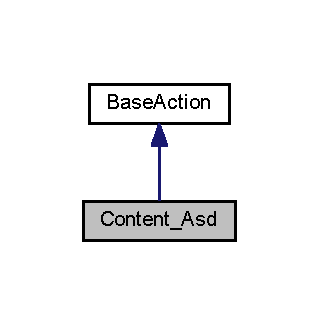
\includegraphics[width=153pt]{class_lora_1_1_content_1_1_content___asd__inherit__graph}
\end{center}
\end{figure}


Collaboration diagram for Content\+\_\+\+Asd\+:\nopagebreak
\begin{figure}[H]
\begin{center}
\leavevmode
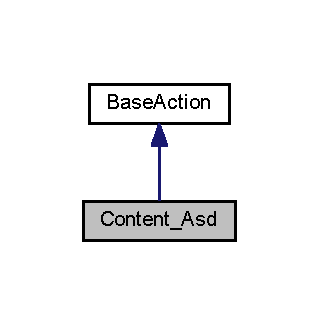
\includegraphics[width=153pt]{class_lora_1_1_content_1_1_content___asd__coll__graph}
\end{center}
\end{figure}
\subsection*{Public Member Functions}
\begin{DoxyCompactItemize}
\item 
\mbox{\label{class_lora_1_1_content_1_1_content___asd_a3ad4bf1b146a3180b34d1327ff2abf69}} 
{\bfseries \+\_\+get} (\textbf{ Request\+Data} \$req)
\item 
\mbox{\label{class_lora_1_1_content_1_1_content___asd_a50751d47a139282d1c3b08cab1b6562e}} 
{\bfseries \+\_\+post} (\textbf{ Request\+Data} \$req)
\item 
\mbox{\label{class_lora_1_1_content_1_1_content___asd_a2affcc8f31c13147c33450193b229194}} 
{\bfseries \+\_\+put} (\textbf{ Request\+Data} \$req)
\item 
\mbox{\label{class_lora_1_1_content_1_1_content___asd_ab8ddc6de1e04524212f7d55893f78864}} 
{\bfseries \+\_\+delete} (\textbf{ Request\+Data} \$req)
\end{DoxyCompactItemize}
\subsection*{Additional Inherited Members}


The documentation for this class was generated from the following file\+:\begin{DoxyCompactItemize}
\item 
servers/webserver/server/content/views/asd/asd.\+php\end{DoxyCompactItemize}

\section{Content\+\_\+\+Device Class Reference}
\label{class_lora_1_1_content_1_1_content___device}\index{Content\+\_\+\+Device@{Content\+\_\+\+Device}}


Inheritance diagram for Content\+\_\+\+Device\+:\nopagebreak
\begin{figure}[H]
\begin{center}
\leavevmode
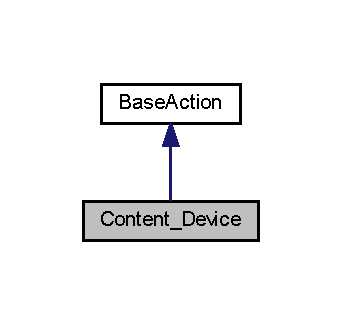
\includegraphics[width=164pt]{class_lora_1_1_content_1_1_content___device__inherit__graph}
\end{center}
\end{figure}


Collaboration diagram for Content\+\_\+\+Device\+:\nopagebreak
\begin{figure}[H]
\begin{center}
\leavevmode
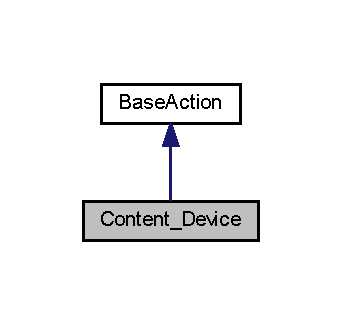
\includegraphics[width=164pt]{class_lora_1_1_content_1_1_content___device__coll__graph}
\end{center}
\end{figure}
\subsection*{Public Member Functions}
\begin{DoxyCompactItemize}
\item 
\mbox{\label{class_lora_1_1_content_1_1_content___device_a3ad4bf1b146a3180b34d1327ff2abf69}} 
{\bfseries \+\_\+get} (\textbf{ Request\+Data} \$req)
\item 
\mbox{\label{class_lora_1_1_content_1_1_content___device_a50751d47a139282d1c3b08cab1b6562e}} 
{\bfseries \+\_\+post} (\textbf{ Request\+Data} \$req)
\item 
\mbox{\label{class_lora_1_1_content_1_1_content___device_a2affcc8f31c13147c33450193b229194}} 
{\bfseries \+\_\+put} (\textbf{ Request\+Data} \$req)
\item 
\mbox{\label{class_lora_1_1_content_1_1_content___device_ab8ddc6de1e04524212f7d55893f78864}} 
{\bfseries \+\_\+delete} (\textbf{ Request\+Data} \$req)
\end{DoxyCompactItemize}
\subsection*{Private Member Functions}
\begin{DoxyCompactItemize}
\item 
\mbox{\label{class_lora_1_1_content_1_1_content___device_a9ff3b3604c524ec2caf3e201ca0ca298}} 
{\bfseries fetch\+Data} (\textbf{ Request\+Data} \$req, \$id)
\end{DoxyCompactItemize}
\subsection*{Additional Inherited Members}


The documentation for this class was generated from the following file\+:\begin{DoxyCompactItemize}
\item 
servers/webserver/server/content/views/device/device.\+php\end{DoxyCompactItemize}

\hypertarget{class_lora_1_1_content_1_1_content___devices}{}\section{Content\+\_\+\+Devices Class Reference}
\label{class_lora_1_1_content_1_1_content___devices}\index{Content\+\_\+\+Devices@{Content\+\_\+\+Devices}}


Inheritance diagram for Content\+\_\+\+Devices\+:
% FIG 0


Collaboration diagram for Content\+\_\+\+Devices\+:
% FIG 1
\subsection*{Public Member Functions}
\begin{DoxyCompactItemize}
\item 
\mbox{\Hypertarget{class_lora_1_1_content_1_1_content___devices_a3ad4bf1b146a3180b34d1327ff2abf69}\label{class_lora_1_1_content_1_1_content___devices_a3ad4bf1b146a3180b34d1327ff2abf69}} 
{\bfseries \+\_\+get} (\hyperlink{class_request_data}{Request\+Data} \$req)
\item 
\mbox{\Hypertarget{class_lora_1_1_content_1_1_content___devices_a50751d47a139282d1c3b08cab1b6562e}\label{class_lora_1_1_content_1_1_content___devices_a50751d47a139282d1c3b08cab1b6562e}} 
{\bfseries \+\_\+post} (\hyperlink{class_request_data}{Request\+Data} \$req)
\item 
\mbox{\Hypertarget{class_lora_1_1_content_1_1_content___devices_a2affcc8f31c13147c33450193b229194}\label{class_lora_1_1_content_1_1_content___devices_a2affcc8f31c13147c33450193b229194}} 
{\bfseries \+\_\+put} (\hyperlink{class_request_data}{Request\+Data} \$req)
\item 
\mbox{\Hypertarget{class_lora_1_1_content_1_1_content___devices_ab8ddc6de1e04524212f7d55893f78864}\label{class_lora_1_1_content_1_1_content___devices_ab8ddc6de1e04524212f7d55893f78864}} 
{\bfseries \+\_\+delete} (\hyperlink{class_request_data}{Request\+Data} \$req)
\end{DoxyCompactItemize}
\subsection*{Private Member Functions}
\begin{DoxyCompactItemize}
\item 
\mbox{\Hypertarget{class_lora_1_1_content_1_1_content___devices_a1a64aa34a50476a8b7e6db0a17fb4975}\label{class_lora_1_1_content_1_1_content___devices_a1a64aa34a50476a8b7e6db0a17fb4975}} 
{\bfseries fetch\+Devices} ()
\end{DoxyCompactItemize}
\subsection*{Additional Inherited Members}


The documentation for this class was generated from the following file\+:\begin{DoxyCompactItemize}
\item 
servers/webserver/server/content/views/devices/devices.\+php\end{DoxyCompactItemize}

\section{Content\+\_\+\+Home Class Reference}
\label{class_lora_1_1_content_1_1_content___home}\index{Content\+\_\+\+Home@{Content\+\_\+\+Home}}


Inheritance diagram for Content\+\_\+\+Home\+:\nopagebreak
\begin{figure}[H]
\begin{center}
\leavevmode
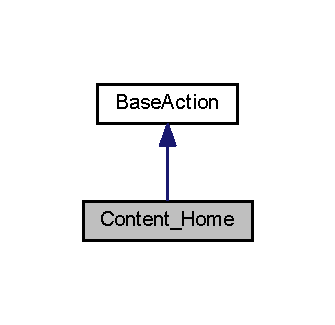
\includegraphics[width=161pt]{class_lora_1_1_content_1_1_content___home__inherit__graph}
\end{center}
\end{figure}


Collaboration diagram for Content\+\_\+\+Home\+:\nopagebreak
\begin{figure}[H]
\begin{center}
\leavevmode
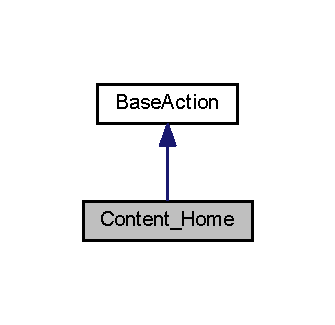
\includegraphics[width=161pt]{class_lora_1_1_content_1_1_content___home__coll__graph}
\end{center}
\end{figure}
\subsection*{Public Member Functions}
\begin{DoxyCompactItemize}
\item 
\mbox{\label{class_lora_1_1_content_1_1_content___home_a3ad4bf1b146a3180b34d1327ff2abf69}} 
{\bfseries \+\_\+get} (\textbf{ Request\+Data} \$req)
\item 
\mbox{\label{class_lora_1_1_content_1_1_content___home_a50751d47a139282d1c3b08cab1b6562e}} 
{\bfseries \+\_\+post} (\textbf{ Request\+Data} \$req)
\item 
\mbox{\label{class_lora_1_1_content_1_1_content___home_a2affcc8f31c13147c33450193b229194}} 
{\bfseries \+\_\+put} (\textbf{ Request\+Data} \$req)
\item 
\mbox{\label{class_lora_1_1_content_1_1_content___home_ab8ddc6de1e04524212f7d55893f78864}} 
{\bfseries \+\_\+delete} (\textbf{ Request\+Data} \$req)
\end{DoxyCompactItemize}
\subsection*{Additional Inherited Members}


The documentation for this class was generated from the following file\+:\begin{DoxyCompactItemize}
\item 
servers/webserver/server/content/views/home/home.\+php\end{DoxyCompactItemize}

\hypertarget{class_lora_1_1_content_1_1_content___info}{}\section{Content\+\_\+\+Info Class Reference}
\label{class_lora_1_1_content_1_1_content___info}\index{Content\+\_\+\+Info@{Content\+\_\+\+Info}}


Inheritance diagram for Content\+\_\+\+Info\+:
% FIG 0


Collaboration diagram for Content\+\_\+\+Info\+:
% FIG 1
\subsection*{Public Member Functions}
\begin{DoxyCompactItemize}
\item 
\mbox{\Hypertarget{class_lora_1_1_content_1_1_content___info_a3ad4bf1b146a3180b34d1327ff2abf69}\label{class_lora_1_1_content_1_1_content___info_a3ad4bf1b146a3180b34d1327ff2abf69}} 
{\bfseries \+\_\+get} (\hyperlink{class_request_data}{Request\+Data} \$req)
\item 
\mbox{\Hypertarget{class_lora_1_1_content_1_1_content___info_a50751d47a139282d1c3b08cab1b6562e}\label{class_lora_1_1_content_1_1_content___info_a50751d47a139282d1c3b08cab1b6562e}} 
{\bfseries \+\_\+post} (\hyperlink{class_request_data}{Request\+Data} \$req)
\item 
\mbox{\Hypertarget{class_lora_1_1_content_1_1_content___info_a2affcc8f31c13147c33450193b229194}\label{class_lora_1_1_content_1_1_content___info_a2affcc8f31c13147c33450193b229194}} 
{\bfseries \+\_\+put} (\hyperlink{class_request_data}{Request\+Data} \$req)
\item 
\mbox{\Hypertarget{class_lora_1_1_content_1_1_content___info_ab8ddc6de1e04524212f7d55893f78864}\label{class_lora_1_1_content_1_1_content___info_ab8ddc6de1e04524212f7d55893f78864}} 
{\bfseries \+\_\+delete} (\hyperlink{class_request_data}{Request\+Data} \$req)
\end{DoxyCompactItemize}
\subsection*{Additional Inherited Members}


The documentation for this class was generated from the following file\+:\begin{DoxyCompactItemize}
\item 
servers/webserver/server/content/views/info/info.\+php\end{DoxyCompactItemize}

\section{Content\+\_\+\+Rtfeed Class Reference}
\label{class_lora_1_1_content_1_1_content___rtfeed}\index{Content\+\_\+\+Rtfeed@{Content\+\_\+\+Rtfeed}}


Inheritance diagram for Content\+\_\+\+Rtfeed\+:\nopagebreak
\begin{figure}[H]
\begin{center}
\leavevmode
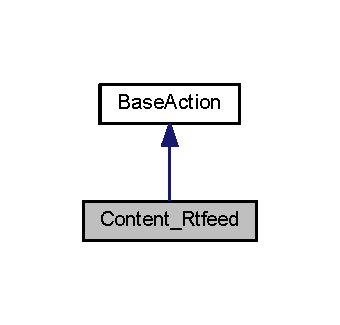
\includegraphics[width=163pt]{class_lora_1_1_content_1_1_content___rtfeed__inherit__graph}
\end{center}
\end{figure}


Collaboration diagram for Content\+\_\+\+Rtfeed\+:\nopagebreak
\begin{figure}[H]
\begin{center}
\leavevmode
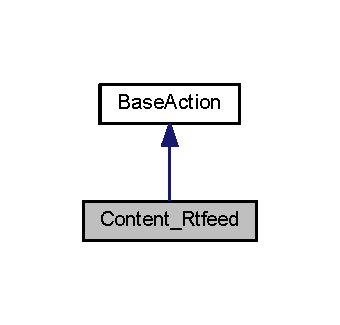
\includegraphics[width=163pt]{class_lora_1_1_content_1_1_content___rtfeed__coll__graph}
\end{center}
\end{figure}
\subsection*{Public Member Functions}
\begin{DoxyCompactItemize}
\item 
\mbox{\label{class_lora_1_1_content_1_1_content___rtfeed_a3ad4bf1b146a3180b34d1327ff2abf69}} 
{\bfseries \+\_\+get} (\textbf{ Request\+Data} \$req)
\item 
\mbox{\label{class_lora_1_1_content_1_1_content___rtfeed_a50751d47a139282d1c3b08cab1b6562e}} 
{\bfseries \+\_\+post} (\textbf{ Request\+Data} \$req)
\item 
\mbox{\label{class_lora_1_1_content_1_1_content___rtfeed_a2affcc8f31c13147c33450193b229194}} 
{\bfseries \+\_\+put} (\textbf{ Request\+Data} \$req)
\item 
\mbox{\label{class_lora_1_1_content_1_1_content___rtfeed_ab8ddc6de1e04524212f7d55893f78864}} 
{\bfseries \+\_\+delete} (\textbf{ Request\+Data} \$req)
\end{DoxyCompactItemize}
\subsection*{Additional Inherited Members}


The documentation for this class was generated from the following file\+:\begin{DoxyCompactItemize}
\item 
servers/webserver/server/content/views/rtfeed/rtfeed.\+php\end{DoxyCompactItemize}

\hypertarget{class_lora_1_1_api_1_1_control_server}{}\section{Control\+Server Class Reference}
\label{class_lora_1_1_api_1_1_control_server}\index{Control\+Server@{Control\+Server}}


Inheritance diagram for Control\+Server\+:
% FIG 0


Collaboration diagram for Control\+Server\+:
% FIG 1
\subsection*{Public Member Functions}
\begin{DoxyCompactItemize}
\item 
\mbox{\Hypertarget{class_lora_1_1_api_1_1_control_server_a038654e8959a00da1dcaab1789a8a73f}\label{class_lora_1_1_api_1_1_control_server_a038654e8959a00da1dcaab1789a8a73f}} 
{\bfseries \+\_\+\+\_\+construct} (\$public\+Server, \$address, \$port)
\end{DoxyCompactItemize}
\subsection*{Data Fields}
\begin{DoxyCompactItemize}
\item 
\mbox{\Hypertarget{class_lora_1_1_api_1_1_control_server_a1d6ddc9c52e0994f2ec85eb34cc1b1cf}\label{class_lora_1_1_api_1_1_control_server_a1d6ddc9c52e0994f2ec85eb34cc1b1cf}} 
{\bfseries \$run} = true
\item 
\mbox{\Hypertarget{class_lora_1_1_api_1_1_control_server_a2543b9ff8834fe7f10c97240667dd121}\label{class_lora_1_1_api_1_1_control_server_a2543b9ff8834fe7f10c97240667dd121}} 
{\bfseries \$public\+Server} = null
\end{DoxyCompactItemize}
\subsection*{Protected Member Functions}
\begin{DoxyCompactItemize}
\item 
\mbox{\Hypertarget{class_lora_1_1_api_1_1_control_server_a805b6933fa0b69978e35fe94f3884de7}\label{class_lora_1_1_api_1_1_control_server_a805b6933fa0b69978e35fe94f3884de7}} 
{\bfseries process} (\$user, \$message)
\item 
\mbox{\Hypertarget{class_lora_1_1_api_1_1_control_server_a3e89014762456a67edbe843811c78736}\label{class_lora_1_1_api_1_1_control_server_a3e89014762456a67edbe843811c78736}} 
{\bfseries connected} (\$user)
\item 
\mbox{\Hypertarget{class_lora_1_1_api_1_1_control_server_aaf6375ec8ee41584a5adcf3d85d73018}\label{class_lora_1_1_api_1_1_control_server_aaf6375ec8ee41584a5adcf3d85d73018}} 
{\bfseries closed} (\$user)
\end{DoxyCompactItemize}
\subsection*{Private Member Functions}
\begin{DoxyCompactItemize}
\item 
\mbox{\Hypertarget{class_lora_1_1_api_1_1_control_server_a14e8d4dad46db8bbfe6c8810a88cf155}\label{class_lora_1_1_api_1_1_control_server_a14e8d4dad46db8bbfe6c8810a88cf155}} 
{\bfseries parse\+Message} (string \$message)
\item 
\mbox{\Hypertarget{class_lora_1_1_api_1_1_control_server_ae6fb713e4c2900de8c57b949020384c3}\label{class_lora_1_1_api_1_1_control_server_ae6fb713e4c2900de8c57b949020384c3}} 
{\bfseries resolve\+Command} (string \$command, string \$data)
\item 
\mbox{\Hypertarget{class_lora_1_1_api_1_1_control_server_aae6d2f0ed43d77087c71ffd4919dcf5d}\label{class_lora_1_1_api_1_1_control_server_aae6d2f0ed43d77087c71ffd4919dcf5d}} 
{\bfseries terminate} ()
\item 
\mbox{\Hypertarget{class_lora_1_1_api_1_1_control_server_ab671527a81a457e51152cc532c716faa}\label{class_lora_1_1_api_1_1_control_server_ab671527a81a457e51152cc532c716faa}} 
{\bfseries broadcast} (string \$command)
\end{DoxyCompactItemize}


The documentation for this class was generated from the following file\+:\begin{DoxyCompactItemize}
\item 
servers/webserver/server/api/socket/socket.\+php\end{DoxyCompactItemize}

\section{Control\+Server Class Reference}
\label{class_lora_1_1_control_server}\index{Control\+Server@{Control\+Server}}


Inheritance diagram for Control\+Server\+:
\nopagebreak
\begin{figure}[H]
\begin{center}
\leavevmode
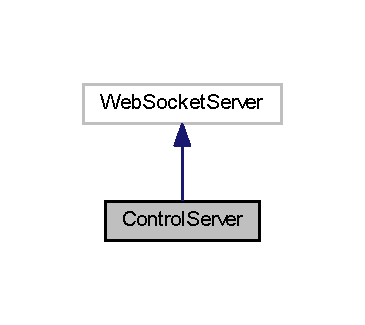
\includegraphics[width=175pt]{class_lora_1_1_control_server__inherit__graph}
\end{center}
\end{figure}


Collaboration diagram for Control\+Server\+:
\nopagebreak
\begin{figure}[H]
\begin{center}
\leavevmode
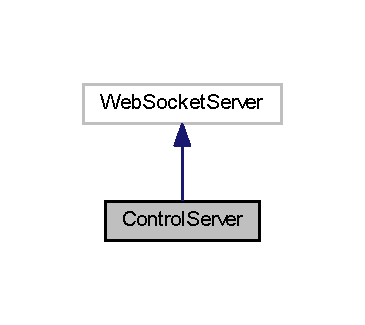
\includegraphics[width=175pt]{class_lora_1_1_control_server__coll__graph}
\end{center}
\end{figure}
\subsection*{Public Member Functions}
\begin{DoxyCompactItemize}
\item 
\mbox{\label{class_lora_1_1_control_server_af1f52d912f7264309f424e05c28b31cb}} 
{\bfseries \+\_\+\+\_\+construct} (\textbf{ Realtime\+Server} \$public\+Server, string \$address, int \$port)
\end{DoxyCompactItemize}
\subsection*{Data Fields}
\begin{DoxyCompactItemize}
\item 
\mbox{\label{class_lora_1_1_control_server_a1d6ddc9c52e0994f2ec85eb34cc1b1cf}} 
{\bfseries \$run} = true
\item 
\mbox{\label{class_lora_1_1_control_server_a2543b9ff8834fe7f10c97240667dd121}} 
{\bfseries \$public\+Server} = null
\end{DoxyCompactItemize}
\subsection*{Protected Member Functions}
\begin{DoxyCompactItemize}
\item 
\mbox{\label{class_lora_1_1_control_server_a805b6933fa0b69978e35fe94f3884de7}} 
{\bfseries process} (\$user, \$message)
\item 
\mbox{\label{class_lora_1_1_control_server_a3e89014762456a67edbe843811c78736}} 
{\bfseries connected} (\$user)
\item 
\mbox{\label{class_lora_1_1_control_server_aaf6375ec8ee41584a5adcf3d85d73018}} 
{\bfseries closed} (\$user)
\end{DoxyCompactItemize}
\subsection*{Private Member Functions}
\begin{DoxyCompactItemize}
\item 
\mbox{\label{class_lora_1_1_control_server_a6523ac8f5d1a8bc4978d80b60193ce73}} 
{\bfseries resolve\+Command} (array \$command, \$user, string \$message)
\item 
\textbf{ terminate} ()
\item 
\textbf{ broadcast} (string \$command)
\end{DoxyCompactItemize}


\subsection{Member Function Documentation}
\mbox{\label{class_lora_1_1_control_server_ab671527a81a457e51152cc532c716faa}} 
\index{Lora\+::\+Control\+Server@{Lora\+::\+Control\+Server}!broadcast@{broadcast}}
\index{broadcast@{broadcast}!Lora\+::\+Control\+Server@{Lora\+::\+Control\+Server}}
\subsubsection{broadcast()}
{\footnotesize\ttfamily broadcast (\begin{DoxyParamCaption}\item[{string}]{\$command }\end{DoxyParamCaption})\hspace{0.3cm}{\ttfamily [private]}}

Broadcast a message to all interested clients. \begin{DoxyRefDesc}{Todo}
\item[\textbf{ Todo}]Write message subscription system. \end{DoxyRefDesc}

\begin{DoxyCode}
63                                                  : \textcolor{keywordtype}{void} \{
64         \textcolor{keywordflow}{if} (empty ($command)) \{
65             \textcolor{keywordflow}{return};
66         \}
67         \textcolor{keywordflow}{foreach} ($this->users as $user) \{
68             \textcolor{keywordflow}{if} ($user->socket !== $this->master) \{
69                 $this->send ($user, $command);
70             \}
71         \}
72     \}
\end{DoxyCode}
\mbox{\label{class_lora_1_1_control_server_aae6d2f0ed43d77087c71ffd4919dcf5d}} 
\index{Lora\+::\+Control\+Server@{Lora\+::\+Control\+Server}!terminate@{terminate}}
\index{terminate@{terminate}!Lora\+::\+Control\+Server@{Lora\+::\+Control\+Server}}
\subsubsection{terminate()}
{\footnotesize\ttfamily terminate (\begin{DoxyParamCaption}{ }\end{DoxyParamCaption})\hspace{0.3cm}{\ttfamily [private]}}

Graceful shotdown routine. Disconnects all clients and finally terminates this process by setting run to false. 
\begin{DoxyCode}
50                                   \{
51         \textcolor{keywordflow}{foreach} ($this->users as $user) \{
52             \textcolor{keywordflow}{if} ($user->socket !== $this->master) \{
53                 $this->disconnect ($user);
54             \}
55         \}
56         $this->run = \textcolor{keyword}{false};
57     \}
\end{DoxyCode}


The documentation for this class was generated from the following file\+:\begin{DoxyCompactItemize}
\item 
servers/rtserver/server/controlserver.\+php\end{DoxyCompactItemize}

\section{D\+AO Class Reference}
\label{class_lora_1_1_d_a_o}\index{D\+AO@{D\+AO}}
\subsection*{Static Public Member Functions}
\begin{DoxyCompactItemize}
\item 
static \textbf{ fetch\+Devices} (array \$projection=[$\,$])
\item 
static \textbf{ device\+Exist} (string \$device\+\_\+id)
\item 
static \textbf{ insert\+Measurement} (string \$device\+\_\+id, int \$time, array \$measurements)
\item 
static \textbf{ insert\+Device} (string \$device)
\item 
static \textbf{ insert\+Raw} (array \$raw)
\end{DoxyCompactItemize}


\subsection{Member Function Documentation}
\mbox{\label{class_lora_1_1_d_a_o_aad2161af4b52afb99e2a931538559823}} 
\index{Lora\+::\+D\+AO@{Lora\+::\+D\+AO}!device\+Exist@{device\+Exist}}
\index{device\+Exist@{device\+Exist}!Lora\+::\+D\+AO@{Lora\+::\+D\+AO}}
\subsubsection{device\+Exist()}
{\footnotesize\ttfamily static device\+Exist (\begin{DoxyParamCaption}\item[{string}]{\$device\+\_\+id }\end{DoxyParamCaption})\hspace{0.3cm}{\ttfamily [static]}}

\begin{DoxyReturn}{Returns}
Returns a boolean indiciation existence of a device. Null is returned is query failed. 
\end{DoxyReturn}

\begin{DoxyCode}
32                                                            : ?\textcolor{keywordtype}{bool} \{
33         \textcolor{keywordflow}{try} \{
34             $manager = \DBConnection::connection (\textcolor{stringliteral}{'measurements'});
35             $command = new \(\backslash\)MongoDB\(\backslash\)Driver\(\backslash\)Command ([
36                 \textcolor{stringliteral}{'count'} => \textcolor{stringliteral}{'devices'},
37                 \textcolor{stringliteral}{'query'} => [
38                     \textcolor{stringliteral}{'\_id'} => $device\_id
39                 ]
40             ]);
41             $cursor = $manager->executeCommand (\textcolor{stringliteral}{'lorawan'}, $command);
42             \textcolor{keywordflow}{return} $cursor->toArray ()[0]->n === 1;
43         \} \textcolor{keywordflow}{catch} (Exception $e) \{
44         \}
45         \textcolor{keywordflow}{return} null;
46     \}
\end{DoxyCode}
Here is the call graph for this function\+:
\nopagebreak
\begin{figure}[H]
\begin{center}
\leavevmode
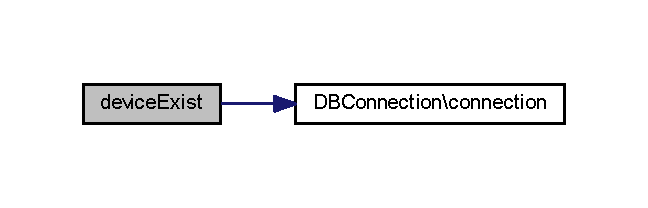
\includegraphics[width=311pt]{class_lora_1_1_d_a_o_aad2161af4b52afb99e2a931538559823_cgraph}
\end{center}
\end{figure}
\mbox{\label{class_lora_1_1_d_a_o_a223eeb00734ccb30b2a83b7557b4dbf1}} 
\index{Lora\+::\+D\+AO@{Lora\+::\+D\+AO}!fetch\+Devices@{fetch\+Devices}}
\index{fetch\+Devices@{fetch\+Devices}!Lora\+::\+D\+AO@{Lora\+::\+D\+AO}}
\subsubsection{fetch\+Devices()}
{\footnotesize\ttfamily static fetch\+Devices (\begin{DoxyParamCaption}\item[{array}]{\$projection = {\ttfamily []} }\end{DoxyParamCaption})\hspace{0.3cm}{\ttfamily [static]}}

Returns an array containing all devices found in the database. 
\begin{DoxyParams}{Parameters}
{\em \$projection} & An optional projection parameter to define the fields which are fetched for each device \\
\hline
\end{DoxyParams}
\begin{DoxyReturn}{Returns}
An array containing all the devices with fields defined by projection. An empty array is returned in case of an error. 
\end{DoxyReturn}

\begin{DoxyCode}
17                                                                  \{
18         $result = [];
19         \textcolor{keywordflow}{try} \{
20             $manager = \DBConnection::connection (\textcolor{stringliteral}{'measurements'});
21             $query = new \(\backslash\)MongoDB\(\backslash\)Driver\(\backslash\)Query ([], [ \textcolor{stringliteral}{'projection'} => $projection ]);
22             $cursor = $manager->executeQuery (\textcolor{stringliteral}{'lorawan.devices'}, $query);
23             $result = $cursor->toArray ();
24         \} \textcolor{keywordflow}{catch} (\(\backslash\)Exception $e) \{
25         \}
26         \textcolor{keywordflow}{return} $result;
27     \}
\end{DoxyCode}
Here is the call graph for this function\+:
\nopagebreak
\begin{figure}[H]
\begin{center}
\leavevmode
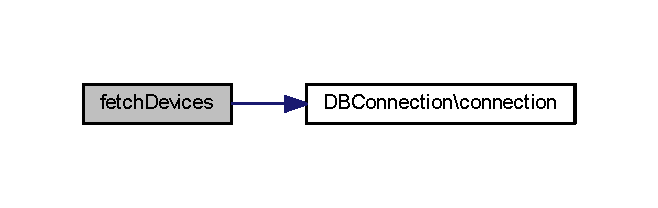
\includegraphics[width=316pt]{class_lora_1_1_d_a_o_a223eeb00734ccb30b2a83b7557b4dbf1_cgraph}
\end{center}
\end{figure}
\mbox{\label{class_lora_1_1_d_a_o_ad231d647bc7bf221289e5e52254d3743}} 
\index{Lora\+::\+D\+AO@{Lora\+::\+D\+AO}!insert\+Device@{insert\+Device}}
\index{insert\+Device@{insert\+Device}!Lora\+::\+D\+AO@{Lora\+::\+D\+AO}}
\subsubsection{insert\+Device()}
{\footnotesize\ttfamily static insert\+Device (\begin{DoxyParamCaption}\item[{string}]{\$device }\end{DoxyParamCaption})\hspace{0.3cm}{\ttfamily [static]}}

Insert a new device or update an existing one. 
\begin{DoxyParams}{Parameters}
{\em \$device} & Device hardware id. \\
\hline
\end{DoxyParams}
\begin{DoxyReturn}{Returns}
True on success, false on error. 
\end{DoxyReturn}

\begin{DoxyCode}
72                                                          : \textcolor{keywordtype}{bool} \{
73         \textcolor{keywordflow}{try} \{
74 \textcolor{preprocessor}{            # Insert device information or update existing.}
75             $manager = \DBConnection::connection (\textcolor{stringliteral}{'measurements'});
76             $writer = \textcolor{keyword}{new} MongoDB\(\backslash\)Driver\(\backslash\)BulkWrite ([ \textcolor{stringliteral}{'ordered'} => \textcolor{keyword}{true} ]);
77             $writer->update ([ \textcolor{stringliteral}{'\_id'} => $device [\textcolor{stringliteral}{'dev'}][\textcolor{stringliteral}{'\_id'}] ], $device [\textcolor{stringliteral}{'dev'}], [ \textcolor{stringliteral}{'upsert'} => \textcolor{keyword}{true} ]);
78             $result = $manager->executeBulkWrite (\textcolor{stringliteral}{'lorawan.devices'}, $writer);
79         \} \textcolor{keywordflow}{catch} (Exception $e) \{
80             \textcolor{keywordflow}{return} \textcolor{keyword}{false};
81         \} \textcolor{keywordflow}{return} \textcolor{keyword}{true};
82     \}
\end{DoxyCode}
Here is the call graph for this function\+:
\nopagebreak
\begin{figure}[H]
\begin{center}
\leavevmode
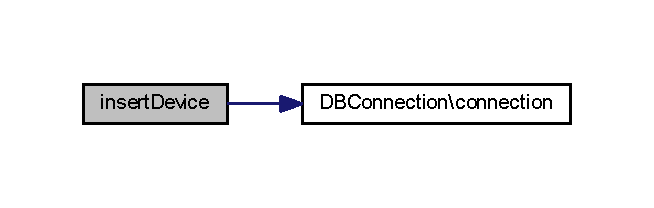
\includegraphics[width=314pt]{class_lora_1_1_d_a_o_ad231d647bc7bf221289e5e52254d3743_cgraph}
\end{center}
\end{figure}
\mbox{\label{class_lora_1_1_d_a_o_ae6bdc6374713a2785aed2fb29c49ca31}} 
\index{Lora\+::\+D\+AO@{Lora\+::\+D\+AO}!insert\+Measurement@{insert\+Measurement}}
\index{insert\+Measurement@{insert\+Measurement}!Lora\+::\+D\+AO@{Lora\+::\+D\+AO}}
\subsubsection{insert\+Measurement()}
{\footnotesize\ttfamily static insert\+Measurement (\begin{DoxyParamCaption}\item[{string}]{\$device\+\_\+id,  }\item[{int}]{\$time,  }\item[{array}]{\$measurements }\end{DoxyParamCaption})\hspace{0.3cm}{\ttfamily [static]}}

Insert a new measurement set for a device. 
\begin{DoxyParams}{Parameters}
{\em \$device\+\_\+id} & Hardware id of the device. \\
\hline
{\em \$time} & Unix timestamp in seconds. \\
\hline
{\em \$measurement} & Measurement data in parsed form. \\
\hline
\end{DoxyParams}
\begin{DoxyReturn}{Returns}
Returns true on succesful insert, false otherwise. 
\end{DoxyReturn}

\begin{DoxyCode}
55                                                                                                  : \textcolor{keywordtype}{bool} \{
56         \textcolor{keywordflow}{try} \{
57 \textcolor{preprocessor}{            # Insert parsed measurement data for actual use.}
58             $manager = \DBConnection::connection (\textcolor{stringliteral}{'measurements'});
59             $writer = \textcolor{keyword}{new} MongoDB\(\backslash\)Driver\(\backslash\)BulkWrite ([ \textcolor{stringliteral}{'ordered'} => \textcolor{keyword}{true} ]);
60             $writer->insert ([ \textcolor{stringliteral}{'device'} => $device\_id, $measurements ]);
61             $result = $manager->executeBulkWrite (\textcolor{stringliteral}{'lorawan.data'}, $writer);
62         \} \textcolor{keywordflow}{catch} (Exception $e) \{
63             \textcolor{keywordflow}{return} \textcolor{keyword}{false};
64         \} \textcolor{keywordflow}{return} \textcolor{keyword}{true};
65     \}
\end{DoxyCode}
Here is the call graph for this function\+:
\nopagebreak
\begin{figure}[H]
\begin{center}
\leavevmode
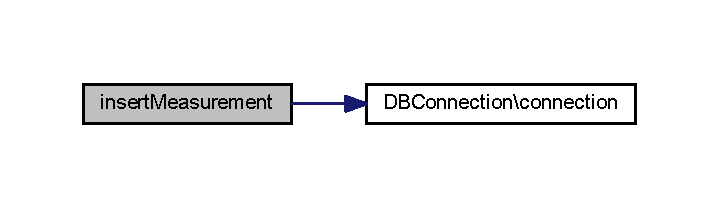
\includegraphics[width=345pt]{class_lora_1_1_d_a_o_ae6bdc6374713a2785aed2fb29c49ca31_cgraph}
\end{center}
\end{figure}
\mbox{\label{class_lora_1_1_d_a_o_aa6d166466386cc6a0147d00719444276}} 
\index{Lora\+::\+D\+AO@{Lora\+::\+D\+AO}!insert\+Raw@{insert\+Raw}}
\index{insert\+Raw@{insert\+Raw}!Lora\+::\+D\+AO@{Lora\+::\+D\+AO}}
\subsubsection{insert\+Raw()}
{\footnotesize\ttfamily static insert\+Raw (\begin{DoxyParamCaption}\item[{array}]{\$raw }\end{DoxyParamCaption})\hspace{0.3cm}{\ttfamily [static]}}

Stores raw data from sensor nodes for archiving and inspection purposes. \begin{DoxyReturn}{Returns}
True on success, false on error. 
\end{DoxyReturn}

\begin{DoxyCode}
88                                                   : \textcolor{keywordtype}{bool} \{
89         \textcolor{keywordflow}{try} \{
90 \textcolor{preprocessor}{            # Insert whole data blob for archiving purposes}
91             $manager = \DBConnection::connection (\textcolor{stringliteral}{'measurements'});
92             $writer = \textcolor{keyword}{new} MongoDB\(\backslash\)Driver\(\backslash\)BulkWrite ([ \textcolor{stringliteral}{'ordered'} => \textcolor{keyword}{true} ]);
93             $writer->insert ($raw);
94             $result = $manager->executeBulkWrite (\textcolor{stringliteral}{'lorawan.raw\_data'}, $writer);
95         \} \textcolor{keywordflow}{catch} (Exception $e) \{
96             \textcolor{keywordflow}{return} \textcolor{keyword}{false};
97         \} \textcolor{keywordflow}{return} \textcolor{keyword}{true};
98     \}
\end{DoxyCode}
Here is the call graph for this function\+:
\nopagebreak
\begin{figure}[H]
\begin{center}
\leavevmode
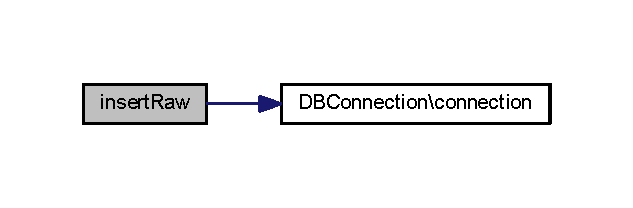
\includegraphics[width=304pt]{class_lora_1_1_d_a_o_aa6d166466386cc6a0147d00719444276_cgraph}
\end{center}
\end{figure}


The documentation for this class was generated from the following file\+:\begin{DoxyCompactItemize}
\item 
lora/dao.\+php\end{DoxyCompactItemize}

\section{Data\+Lib Class Reference}
\label{class_data_lib}\index{Data\+Lib@{Data\+Lib}}
\subsection*{Static Public Member Functions}
\begin{DoxyCompactItemize}
\item 
\mbox{\label{class_data_lib_a13d18479fbd2ba6266e58aff32f0937d}} 
static {\bfseries is\+Json} (string \$value)
\item 
\mbox{\label{class_data_lib_a8550f4875faca7b33f2aff29e6d5066a}} 
static {\bfseries is\+Hex\+String} (string \$val)
\item 
static \textbf{ Is\+Instance\+Of} (\$object, string \$class)
\item 
static \textbf{ Are\+Instance\+Of} (array \$objects, string \$class)
\item 
static \textbf{ is\+Int} (\$value)
\end{DoxyCompactItemize}


\subsection{Detailed Description}
A library for hosting data inspection, verification and sanitazition functions. 

\subsection{Member Function Documentation}
\mbox{\label{class_data_lib_a2bff9a99c41391c309a7618d522c8f16}} 
\index{Data\+Lib@{Data\+Lib}!Are\+Instance\+Of@{Are\+Instance\+Of}}
\index{Are\+Instance\+Of@{Are\+Instance\+Of}!Data\+Lib@{Data\+Lib}}
\subsubsection{Are\+Instance\+Of()}
{\footnotesize\ttfamily static Are\+Instance\+Of (\begin{DoxyParamCaption}\item[{array}]{\$objects,  }\item[{string}]{\$class }\end{DoxyParamCaption})\hspace{0.3cm}{\ttfamily [static]}}

Sees if all items in an array are instances of certain class. 
\begin{DoxyParams}{Parameters}
{\em \$objects} & An array of objects to test. \\
\hline
{\em \$class} & A class name to test each object against. \\
\hline
\end{DoxyParams}
\begin{DoxyReturn}{Returns}
Returns true if and only if all the items in \$objects are instances of \$class and there are more then 0 items in \$objects. False is returned otherwise. 
\end{DoxyReturn}

\begin{DoxyCode}
36                                                                          : \textcolor{keywordtype}{bool} \{
37         \textcolor{keywordflow}{if} (!class\_exists ($class, \textcolor{keyword}{false})) \{
38             \textcolor{keywordflow}{return} \textcolor{keyword}{false};
39         \}
40         \textcolor{keywordflow}{foreach} ($objects as $object) \{
41             \textcolor{keywordflow}{if} (!($object instanceof $class)) \{
42                 \textcolor{keywordflow}{return} \textcolor{keyword}{false};
43             \}
44         \} \textcolor{keywordflow}{return} count ($objects) > 0;
45     \}
\end{DoxyCode}
Here is the caller graph for this function\+:\nopagebreak
\begin{figure}[H]
\begin{center}
\leavevmode
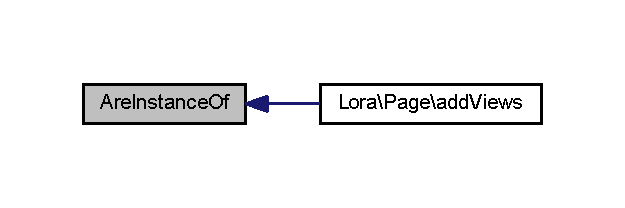
\includegraphics[width=300pt]{class_data_lib_a2bff9a99c41391c309a7618d522c8f16_icgraph}
\end{center}
\end{figure}
\mbox{\label{class_data_lib_a4ab5c189422f1366403e4375a42673d1}} 
\index{Data\+Lib@{Data\+Lib}!Is\+Instance\+Of@{Is\+Instance\+Of}}
\index{Is\+Instance\+Of@{Is\+Instance\+Of}!Data\+Lib@{Data\+Lib}}
\subsubsection{Is\+Instance\+Of()}
{\footnotesize\ttfamily static Is\+Instance\+Of (\begin{DoxyParamCaption}\item[{}]{\$object,  }\item[{string}]{\$class }\end{DoxyParamCaption})\hspace{0.3cm}{\ttfamily [static]}}

Sees if a variable is intance of certain class. 
\begin{DoxyParams}{Parameters}
{\em \$object} & A mixed value to test. \\
\hline
{\em \$class} & A class name to test \$object against. \\
\hline
\end{DoxyParams}
\begin{DoxyReturn}{Returns}
Returns boolean true if \$object is instance of \$class and false if not. 
\end{DoxyReturn}

\begin{DoxyCode}
24                                                                  : \textcolor{keywordtype}{bool} \{
25         \textcolor{keywordflow}{if} (!class\_exists ($class, \textcolor{keyword}{false})) \{
26             \textcolor{keywordflow}{return} \textcolor{keyword}{false};
27         \} \textcolor{keywordflow}{return} $object instanceof $class;
28     \}
\end{DoxyCode}
\mbox{\label{class_data_lib_a60cb59e0d64619154c155046e6e4ca66}} 
\index{Data\+Lib@{Data\+Lib}!is\+Int@{is\+Int}}
\index{is\+Int@{is\+Int}!Data\+Lib@{Data\+Lib}}
\subsubsection{is\+Int()}
{\footnotesize\ttfamily static is\+Int (\begin{DoxyParamCaption}\item[{}]{\$value }\end{DoxyParamCaption})\hspace{0.3cm}{\ttfamily [static]}}

A wrapper function for filter\+\_\+var filtering integers. 
\begin{DoxyParams}{Parameters}
{\em \$value} & A value to test. \\
\hline
\end{DoxyParams}
\begin{DoxyReturn}{Returns}
Returns filtered \$value as an integer if it can be converted and false if not. 
\end{DoxyReturn}

\begin{DoxyCode}
52                                           \{
53         \textcolor{keywordflow}{return} filter\_var ($value, FILTER\_VALIDATE\_INT);
54     \}
\end{DoxyCode}
Here is the caller graph for this function\+:
\nopagebreak
\begin{figure}[H]
\begin{center}
\leavevmode
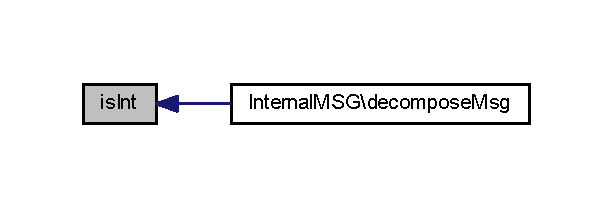
\includegraphics[width=294pt]{class_data_lib_a60cb59e0d64619154c155046e6e4ca66_icgraph}
\end{center}
\end{figure}


The documentation for this class was generated from the following file\+:\begin{DoxyCompactItemize}
\item 
lora/util/datalib.\+php\end{DoxyCompactItemize}

\section{Data\+Server Class Reference}
\label{class_lora_1_1_data_server}\index{Data\+Server@{Data\+Server}}
\subsection*{Public Member Functions}
\begin{DoxyCompactItemize}
\item 
\textbf{ start} ()
\item 
\textbf{ process} (string \$topic, string \$msg)
\end{DoxyCompactItemize}
\subsection*{Static Public Member Functions}
\begin{DoxyCompactItemize}
\item 
\mbox{\label{class_lora_1_1_data_server_a0deb004950b8dc4f51836316fd19c111}} 
static {\bfseries instance} ()
\item 
static \textbf{ process\+Message} (\$topic, \$msg)
\end{DoxyCompactItemize}
\subsection*{Data Fields}
\begin{DoxyCompactItemize}
\item 
\mbox{\label{class_lora_1_1_data_server_af213a81daaf386c089bb36f148cfbd96}} 
{\bfseries \$rt\+\_\+client} = null
\item 
\mbox{\label{class_lora_1_1_data_server_a721b31e1995c24214da0e89eb5ec3100}} 
{\bfseries \$rt\+\_\+address} = \textquotesingle{}\textquotesingle{}
\item 
\mbox{\label{class_lora_1_1_data_server_aaf8416d215d1e9710dfe026490c998dc}} 
{\bfseries \$allow\+Print} = true
\end{DoxyCompactItemize}
\subsection*{Private Member Functions}
\begin{DoxyCompactItemize}
\item 
\textbf{ broadcast} (array \$msg, array \&\$messages)
\item 
\textbf{ parse\+Received} (string \$topic, string \$msg, array \&\$parsed\+Topic, array \&\$parsed\+Msg)
\item 
\textbf{ parse\+Topic} (string \$topic)
\item 
\textbf{ parse\+Message} (\textbackslash{}\textbf{ Request\+Data} \$req)
\item 
\textbf{ parse\+Activation} (\textbackslash{}\textbf{ Request\+Data} \$req)
\item 
\textbf{ parse\+Payload} (string \$payload)
\item 
\mbox{\label{class_lora_1_1_data_server_aa22496921de05f8626d82a7530fcc517}} 
{\bfseries rt\+Connect} ()
\item 
\mbox{\label{class_lora_1_1_data_server_af355edd34f94d0643a98664a966a9658}} 
{\bfseries M\+Q\+T\+T\+Connect} ()
\item 
\textbf{ insert} (string \$device\+Id, array \$data)
\item 
\mbox{\label{class_lora_1_1_data_server_ae86e92ed03b6395cfc4cb99e2371e14a}} 
{\bfseries print} (\$msg, \$eol=true)
\item 
\mbox{\label{class_lora_1_1_data_server_aca780669b9640bfb9f17dcbb11e592d1}} 
{\bfseries print\+All} (array \$msgs)
\end{DoxyCompactItemize}
\subsection*{Private Attributes}
\begin{DoxyCompactItemize}
\item 
\mbox{\label{class_lora_1_1_data_server_a5946274cba635d6d4e49d93b66aa1964}} 
{\bfseries \$mqtt\+\_\+client} = null
\end{DoxyCompactItemize}
\subsection*{Static Private Attributes}
\begin{DoxyCompactItemize}
\item 
\mbox{\label{class_lora_1_1_data_server_ad9d7ce33ebb142b70e58b68052ca0ea8}} 
static {\bfseries \$instance}
\end{DoxyCompactItemize}


\subsection{Detailed Description}
T\+O\+DO\+: Maybe add a buffer for failed broadcasts so that they can be sent later on again. A singleton based class for managing M\+Q\+TT connection to The Things Network and broadcasting data to the system. 

\subsection{Member Function Documentation}
\mbox{\label{class_lora_1_1_data_server_a883eaf25eb21a0ba827bb9a9a3593861}} 
\index{Lora\+::\+Data\+Server@{Lora\+::\+Data\+Server}!broadcast@{broadcast}}
\index{broadcast@{broadcast}!Lora\+::\+Data\+Server@{Lora\+::\+Data\+Server}}
\subsubsection{broadcast()}
{\footnotesize\ttfamily broadcast (\begin{DoxyParamCaption}\item[{array}]{\$msg,  }\item[{array \&}]{\$messages }\end{DoxyParamCaption})\hspace{0.3cm}{\ttfamily [private]}}

\begin{DoxyRefDesc}{Todo}
\item[\textbf{ Todo}]Internal message processing (terminate). Broadcasts a received message to other server systems. Only interested one at the moment is the realtime sever which in turn broadcasts it onwards to clients who are interested in it. \end{DoxyRefDesc}

\begin{DoxyParams}{Parameters}
{\em \$msg} & Parsed M\+Q\+TT message payload with device id and time stamp. \\
\hline
{\em \$messages} & Messages array to allow this method add messages about the data processing. \\
\hline
\end{DoxyParams}
\begin{DoxyReturn}{Returns}
Returns true if the data was succesfully broadcasted and false if not. 
\end{DoxyReturn}

\begin{DoxyCode}
100                                                               : \textcolor{keywordtype}{bool} \{
101         \textcolor{keywordflow}{if} (!$this->rt\_client) \{
102             $messages [] = \textcolor{stringliteral}{"Establishing realtime server connection; \{$this->rt\_address\}"};
103             \textcolor{keywordflow}{if} (!$this->rtConnect ()) \{
104                 $messages [] = \textcolor{stringliteral}{"Could not establish realtime connection."};
105                 \textcolor{keywordflow}{return} \textcolor{keyword}{false};
106             \}
107             $messages [] = \textcolor{stringliteral}{"Realtime connection established."};
108         \}
109         $messages [] = \textcolor{stringliteral}{"Broadcasting data."};
110         $data = InternalMSG::composeMsg (Command::DATA, $msg);
111         \textcolor{keywordflow}{if} (!$this->rt\_client->send ($data)) \{
112             \textcolor{keywordflow}{if} (!$this->rt\_client->isConnected ()) \{
113                 $messages [] = \textcolor{stringliteral}{"Realtime client connection error: "}.$this->rt\_client->lastError ();
114             \}
115             \textcolor{keywordflow}{return} \textcolor{keyword}{false};
116         \}
117         $this->rt\_client->receive ($response);
118         \textcolor{keywordflow}{if} ($response === \textcolor{stringliteral}{'terminate'}) \{
119             $this->rt\_client->close ();
120             \textcolor{keywordflow}{return} \textcolor{keyword}{false};
121         \}
122         $messages [] = \textcolor{stringliteral}{"Response: $\{response\}"};
123         \textcolor{keywordflow}{return} \textcolor{keyword}{true};
124     \}
\end{DoxyCode}
Here is the call graph for this function\+:
\nopagebreak
\begin{figure}[H]
\begin{center}
\leavevmode
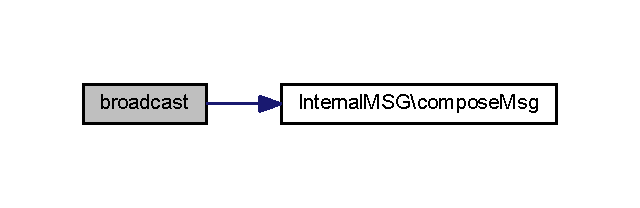
\includegraphics[width=307pt]{class_lora_1_1_data_server_a883eaf25eb21a0ba827bb9a9a3593861_cgraph}
\end{center}
\end{figure}
\mbox{\label{class_lora_1_1_data_server_a6502357e2b91bc3e73f34ec4233b60d3}} 
\index{Lora\+::\+Data\+Server@{Lora\+::\+Data\+Server}!insert@{insert}}
\index{insert@{insert}!Lora\+::\+Data\+Server@{Lora\+::\+Data\+Server}}
\subsubsection{insert()}
{\footnotesize\ttfamily insert (\begin{DoxyParamCaption}\item[{string}]{\$device\+Id,  }\item[{array}]{\$data }\end{DoxyParamCaption})\hspace{0.3cm}{\ttfamily [private]}}

A context aware method for inserting data into database. Checks for the presence of certain values in \$data and uses that information to determine if data should be inserted or not. 
\begin{DoxyParams}{Parameters}
{\em \$device\+Id} & Device hardware id. \\
\hline
{\em \$data} & An array containing parsed M\+Q\+TT originated data. \\
\hline
\end{DoxyParams}
\begin{DoxyReturn}{Returns}
Returns true on success and false if an erro occured. 
\end{DoxyReturn}

\begin{DoxyCode}
279                                                             : \textcolor{keywordtype}{bool} \{
280         $result = DAO::insertDevice ($deviceId);
281         \textcolor{keywordflow}{if} (isset ($data [\textcolor{stringliteral}{'msg'}])) \{
282             $result &= DAO::insertRaw ($data);
283         \}
284         \textcolor{keywordflow}{if} (isset ($data [\textcolor{stringliteral}{'msg'}][\textcolor{stringliteral}{'payload'}], $data [\textcolor{stringliteral}{'msg'}][\textcolor{stringliteral}{'time'}])) \{
285             $result &= DAO::insertMeasurement ($deviceId, $data [\textcolor{stringliteral}{'msg'}][\textcolor{stringliteral}{'time'}], $data [\textcolor{stringliteral}{'msg'}][\textcolor{stringliteral}{'payload'}]);
286         \}
287         \textcolor{keywordflow}{return} $result;
288     \}
\end{DoxyCode}
\mbox{\label{class_lora_1_1_data_server_a48fb1fc7a81a6cf12d17e919e7d724c0}} 
\index{Lora\+::\+Data\+Server@{Lora\+::\+Data\+Server}!parse\+Activation@{parse\+Activation}}
\index{parse\+Activation@{parse\+Activation}!Lora\+::\+Data\+Server@{Lora\+::\+Data\+Server}}
\subsubsection{parse\+Activation()}
{\footnotesize\ttfamily parse\+Activation (\begin{DoxyParamCaption}\item[{\textbackslash{}\textbf{ Request\+Data}}]{\$req }\end{DoxyParamCaption})\hspace{0.3cm}{\ttfamily [private]}}

A case specific parser for an activation message. \doxyref{Data\+Server\+::parse\+Message}{p.}{class_lora_1_1_data_server_ac16e17dca8edf6daf34e403654f9c2c2} cannot parse this without unreasonably large changes so it is wrapped as its own function. 
\begin{DoxyParams}{Parameters}
{\em \$req} & An instance of \doxyref{Request\+Data}{p.}{class_request_data} wrapping the M\+Q\+TT message. \\
\hline
\end{DoxyParams}
\begin{DoxyReturn}{Returns}
Returns a nullable array. An array of parsed data is returned on success and null if the message cannot be parsed. 
\end{DoxyReturn}

\begin{DoxyCode}
220                                                          : ?array \{
221         $required = [
222             \textcolor{stringliteral}{'dev\_eui'}
223         ];
224         $hwId = $req->getString (\textcolor{stringliteral}{'dev\_eui'}, \textcolor{stringliteral}{''});
225         \textcolor{keywordflow}{if} (!$req->has ($required) || !DataLib::isHexString ($hwId)) \{
226             \textcolor{keywordflow}{return} null;
227         \}
228         \textcolor{keywordflow}{return} [ \textcolor{stringliteral}{'device'} => [ \textcolor{stringliteral}{'\_id'} => $hwId ] ];
229     \}
\end{DoxyCode}
\mbox{\label{class_lora_1_1_data_server_ac16e17dca8edf6daf34e403654f9c2c2}} 
\index{Lora\+::\+Data\+Server@{Lora\+::\+Data\+Server}!parse\+Message@{parse\+Message}}
\index{parse\+Message@{parse\+Message}!Lora\+::\+Data\+Server@{Lora\+::\+Data\+Server}}
\subsubsection{parse\+Message()}
{\footnotesize\ttfamily parse\+Message (\begin{DoxyParamCaption}\item[{\textbackslash{}\textbf{ Request\+Data}}]{\$req }\end{DoxyParamCaption})\hspace{0.3cm}{\ttfamily [private]}}

Parses the M\+Q\+TT messaage and ensures precense of required value as well as their type correctness. 
\begin{DoxyParams}{Parameters}
{\em \$req} & An instance of \doxyref{Request\+Data}{p.}{class_request_data} wrapping the M\+Q\+TT message. \\
\hline
\end{DoxyParams}
\begin{DoxyReturn}{Returns}
Returns a nullable array. An array of parsed data is returned on success and null if the message cannot be parsed. 
\end{DoxyReturn}

\begin{DoxyCode}
171                                                       : ?array \{
172         $required = [
173             \textcolor{stringliteral}{'metadata'},
174             \textcolor{stringliteral}{'dev\_id'},
175             \textcolor{stringliteral}{'hardware\_serial'},
176             \textcolor{stringliteral}{'payload\_raw'}
177         ];
178         $requiredMeta = [
179             \textcolor{stringliteral}{'time'}
180         ];
181         \textcolor{keywordflow}{if} (!$req->has ($required)) \{
182             \textcolor{keywordflow}{return} $this->parseActivation ($data);
183         \}
184         \textcolor{keywordflow}{if} ($req->readArray (\textcolor{stringliteral}{'metadata'}, $meta)) \{
185             \textcolor{keywordflow}{return} null;
186         \}
187         $meta = \textcolor{keyword}{new} RequestData ($meta);
188         \textcolor{keywordflow}{if} (!$meta->has ($requiredMeta)) \{
189             \textcolor{keywordflow}{return} null;
190         \}
191         $req->readString (\textcolor{stringliteral}{'dev\_id'}, $devId, \textcolor{stringliteral}{''});
192         $req->readString (\textcolor{stringliteral}{'hardware\_serial'}, $hwId, \textcolor{stringliteral}{''});
193         $payload = $this->parsePayload ($req->getString (\textcolor{stringliteral}{'payload\_raw'}, \textcolor{stringliteral}{''}));
194         $datetime = DateTime::createFromFormat (\textcolor{stringliteral}{'Y-m-d\(\backslash\)TH:i:s+'}, $meta->getString (\textcolor{stringliteral}{'time'}, \textcolor{stringliteral}{''}));
195         \textcolor{keywordflow}{if} ($datetime === \textcolor{keyword}{false} || $payload === null || !DataLib::isHexString ($hwId)) \{
196             \textcolor{keywordflow}{return} null;
197         \}
198         $result = [
199             \textcolor{stringliteral}{'device'} => [
200                 \textcolor{stringliteral}{'\_id'}               => $hwId,
201                 \textcolor{stringliteral}{'dev\_id'}            => $devId,
202                 \textcolor{stringliteral}{'hardware\_serial'}   => $hwId
203             ],
204             \textcolor{stringliteral}{'msg'} => [
205                 \textcolor{stringliteral}{'device\_id'}         => $hwId,
206                 \textcolor{stringliteral}{'time'}              => $datatime->getTimestamp (),
207                 \textcolor{stringliteral}{'payload'}           => $payload
208             ]
209         ];
210         \textcolor{keywordflow}{return} $result;
211     \}
\end{DoxyCode}
\mbox{\label{class_lora_1_1_data_server_a67382ebb6b28ebe3ad81d2f0ae541a84}} 
\index{Lora\+::\+Data\+Server@{Lora\+::\+Data\+Server}!parse\+Payload@{parse\+Payload}}
\index{parse\+Payload@{parse\+Payload}!Lora\+::\+Data\+Server@{Lora\+::\+Data\+Server}}
\subsubsection{parse\+Payload()}
{\footnotesize\ttfamily parse\+Payload (\begin{DoxyParamCaption}\item[{string}]{\$payload }\end{DoxyParamCaption})\hspace{0.3cm}{\ttfamily [private]}}

A method to parse the raw payload data from the M\+Q\+TT server. 
\begin{DoxyParams}{Parameters}
{\em \$payload} & Raw payload string in base64 encoded form. \\
\hline
\end{DoxyParams}
\begin{DoxyReturn}{Returns}
Returns null on failure and an array of associative arrays containing type value pairs of the measured values. 
\end{DoxyReturn}

\begin{DoxyCode}
237                                                     : ?array \{
238         \textcolor{keywordflow}{if} (($payload = base64\_decode ($payload)) === \textcolor{keyword}{false}) \{
239             \textcolor{keywordflow}{return} null;
240         \}
241         $data = explode (\textcolor{charliteral}{'|'}, $payload);
242         $result = [];
243         \textcolor{keywordflow}{foreach} ($data as $key => $entry) \{
244             \textcolor{keywordflow}{if} (empty ($entry)) \{
245                 unset ($data [$key]);
246                 \textcolor{keywordflow}{continue};
247             \}
248             $type = substr ($entry, 0, 3);
249             $value = substr ($entry, 3);
250             $result [] = [ $type => floatval ($value) ];
251         \}
252         \textcolor{keywordflow}{return} $result;
253     \}
\end{DoxyCode}
\mbox{\label{class_lora_1_1_data_server_afc5d093aad072fb26010dc33782491e1}} 
\index{Lora\+::\+Data\+Server@{Lora\+::\+Data\+Server}!parse\+Received@{parse\+Received}}
\index{parse\+Received@{parse\+Received}!Lora\+::\+Data\+Server@{Lora\+::\+Data\+Server}}
\subsubsection{parse\+Received()}
{\footnotesize\ttfamily parse\+Received (\begin{DoxyParamCaption}\item[{string}]{\$topic,  }\item[{string}]{\$msg,  }\item[{array \&}]{\$parsed\+Topic,  }\item[{array \&}]{\$parsed\+Msg }\end{DoxyParamCaption})\hspace{0.3cm}{\ttfamily [private]}}

Parses the topic and message received from the M\+Q\+TT server into more flexible form for this class to use. 
\begin{DoxyParams}[1]{Parameters}
 & {\em \$topic} & Topic received from the M\+Q\+TT server. \\
\hline
 & {\em \$msg} & Message receieved from the M\+Q\+TT server. \\
\hline
\mbox{\tt out}  & {\em \$parsed\+Topic} & An array to which the parsed topic data will be set. Set to null if it cannot be parsed. \\
\hline
\mbox{\tt out}  & {\em \$parsed\+Msg} & An array to which the parsed message data will be set. Set to null if it cannot be parsed. \\
\hline
\end{DoxyParams}
\begin{DoxyReturn}{Returns}
Returns true if parsing was succesful and false if not. 
\end{DoxyReturn}

\begin{DoxyCode}
134                                                                                                         : \textcolor{keywordtype}{
      bool} \{
135         $msg = json\_decode ($msg, \textcolor{keyword}{true});
136         $parsedTopic = $this->parseTopic ($topic);
137         $parsedMsg = $this->parseMessage (\textcolor{keyword}{new} \(\backslash\)RequestData ($msg));
138         \textcolor{keywordflow}{return} $parsedTopic !== null && $parsedMsg !== null;
139     \}
\end{DoxyCode}
\mbox{\label{class_lora_1_1_data_server_a5443eb6d2b44355a72718463885b4631}} 
\index{Lora\+::\+Data\+Server@{Lora\+::\+Data\+Server}!parse\+Topic@{parse\+Topic}}
\index{parse\+Topic@{parse\+Topic}!Lora\+::\+Data\+Server@{Lora\+::\+Data\+Server}}
\subsubsection{parse\+Topic()}
{\footnotesize\ttfamily parse\+Topic (\begin{DoxyParamCaption}\item[{string}]{\$topic }\end{DoxyParamCaption})\hspace{0.3cm}{\ttfamily [private]}}

Parses M\+Q\+TT topic string into an associative array. 
\begin{DoxyParams}{Parameters}
{\em \$topic} & An M\+Q\+TT topic. \\
\hline
\end{DoxyParams}
\begin{DoxyReturn}{Returns}
Returns an associative array containing the topic information. 
\end{DoxyReturn}

\begin{DoxyCode}
146                                                 : array \{
147         $topic = explode (\textcolor{charliteral}{'/'}, $topic);
148         $keys = [
149             \textcolor{stringliteral}{'application'},
150             \textcolor{stringliteral}{'source'},
151             \textcolor{stringliteral}{'device'},
152             \textcolor{stringliteral}{'message'},
153             \textcolor{stringliteral}{'event'}
154         ];
155         \textcolor{keywordflow}{foreach} ($topic as $key => $value) \{
156             \textcolor{keywordflow}{if} (!isset ($keys [$key])) \{
157                 \textcolor{keywordflow}{continue};
158             \}
159             $topic [$keys [$key]] = $value;
160             unset ($topic [$key]);
161         \}
162         \textcolor{keywordflow}{return} $topic;
163     \}
\end{DoxyCode}
\mbox{\label{class_lora_1_1_data_server_acf279a7b53dd92327b68f3b3f376ee2f}} 
\index{Lora\+::\+Data\+Server@{Lora\+::\+Data\+Server}!process@{process}}
\index{process@{process}!Lora\+::\+Data\+Server@{Lora\+::\+Data\+Server}}
\subsubsection{process()}
{\footnotesize\ttfamily process (\begin{DoxyParamCaption}\item[{string}]{\$topic,  }\item[{string}]{\$msg }\end{DoxyParamCaption})}

Main processing method. Parses, stores and broadcasts the received data. 
\begin{DoxyParams}{Parameters}
{\em \$topic} & Topic of the M\+Q\+TT messagae. \\
\hline
{\em \$msg} & Message received from the M\+Q\+TT server. \\
\hline
\end{DoxyParams}
\begin{DoxyReturn}{Returns}
An array of messages is returned describing the processing of the message. 
\end{DoxyReturn}

\begin{DoxyCode}
76                                                          : array \{
77         $messages = [];
78         $messages [] = \textcolor{stringliteral}{"Message received: "}.date (\textcolor{stringliteral}{"r"}).\textcolor{stringliteral}{"\(\backslash\)nTopic:$\{topic\}\(\backslash\)n$\{msg\}\(\backslash\)n"};
79         \textcolor{keywordflow}{if} (!$this->parseReceived ($topic, $msg, $parsedTopic, $parsedMsg)) \{
80             $messages [] = \textcolor{stringliteral}{"Failed to parse message."};
81             \textcolor{keywordflow}{return} $messages;
82         \}
83         \textcolor{keywordflow}{if} (strtolower ($parsedMsg [\textcolor{stringliteral}{'msg'}][\textcolor{stringliteral}{'payload'}]) === \textcolor{stringliteral}{'heartbeat'}) \{
84             \textcolor{keywordflow}{return} $messages;
85         \}
86         $parsedMsg [\textcolor{stringliteral}{'topic'}] = $parsedTopic;
87         $this->insert ($parsedMsg [\textcolor{stringliteral}{'device'}][\textcolor{stringliteral}{'\_id'}], $parsedMsg);
88         $this->broadcast ($parsedMsg [\textcolor{stringliteral}{'msg'}], $messages);
89         \textcolor{keywordflow}{return} $messages;
90     \}
\end{DoxyCode}
\mbox{\label{class_lora_1_1_data_server_a4b928f64ca70f6b6d9bb388bc943ff3f}} 
\index{Lora\+::\+Data\+Server@{Lora\+::\+Data\+Server}!process\+Message@{process\+Message}}
\index{process\+Message@{process\+Message}!Lora\+::\+Data\+Server@{Lora\+::\+Data\+Server}}
\subsubsection{process\+Message()}
{\footnotesize\ttfamily static process\+Message (\begin{DoxyParamCaption}\item[{}]{\$topic,  }\item[{}]{\$msg }\end{DoxyParamCaption})\hspace{0.3cm}{\ttfamily [static]}}

A static entry point to message processing routine. Performs primitive validity checks on data types to see if it is the data is even remotely processable. Proper data sanity checks are done later. 
\begin{DoxyParams}{Parameters}
{\em \$topic} & Topic of the M\+Q\+TT message. \\
\hline
{\em \$msg} & Message received from the M\+Q\+TT server. \\
\hline
\end{DoxyParams}

\begin{DoxyCode}
60                                                          : \textcolor{keywordtype}{void} \{
61         $temp = self::instance ();
62         \textcolor{keywordflow}{if} (!is\_string ($topic) || !is\_string ($msg) || !DataLib::isJson ($msg)) \{
63             $temp->print (\textcolor{stringliteral}{"Invalid message received."});
64             \textcolor{keywordflow}{return};
65         \}
66         $messages = $temp->process ($topic, $msg);
67         $temp->printAll ($messages);
68     \}
\end{DoxyCode}
\mbox{\label{class_lora_1_1_data_server_af8fa59992209e36dccb3eefb0f75531f}} 
\index{Lora\+::\+Data\+Server@{Lora\+::\+Data\+Server}!start@{start}}
\index{start@{start}!Lora\+::\+Data\+Server@{Lora\+::\+Data\+Server}}
\subsubsection{start()}
{\footnotesize\ttfamily start (\begin{DoxyParamCaption}{ }\end{DoxyParamCaption})}

Start the server loop. This is a blocking wait function. 
\begin{DoxyCode}
35                              : \textcolor{keywordtype}{void} \{
36         $this->print (\textcolor{stringliteral}{"Establishing TTN connection."});
37         \textcolor{keywordflow}{if} (!$this->MQTTConnect ()) \{
38             $this->print (\textcolor{stringliteral}{"Could not establish connection to TTN."});
39             \textcolor{keywordflow}{return};
40         \}
41         $this->print (\textcolor{stringliteral}{"Connection to TTN server established. Subscribing to channels..."});
42         $topics [\textcolor{charliteral}{'#'}] = [
43             \textcolor{stringliteral}{"qos"} => 0,
44             \textcolor{stringliteral}{"function"} => \textcolor{stringliteral}{"\(\backslash\)Lora\(\backslash\)DataServer::processMessage"}
45         ];
46         $this->mqtt\_client->subscribe ($topics);
47         \textcolor{comment}{// $this->mqtt\_client->debug = true;}
48         $this->print (\textcolor{stringliteral}{"Subscribing complete. Listening for messages."}.PHP\_EOL);
49         \textcolor{keywordflow}{while} ($this->mqtt\_client->proc ());
50         $this->mqtt\_client->close ();
51         $this->rt\_client->close ();
52     \}
\end{DoxyCode}


The documentation for this class was generated from the following file\+:\begin{DoxyCompactItemize}
\item 
servers/mqttserver/server/dataserver.\+php\end{DoxyCompactItemize}

\section{D\+B\+Connection Class Reference}
\label{class_d_b_connection}\index{D\+B\+Connection@{D\+B\+Connection}}
\subsection*{Static Public Member Functions}
\begin{DoxyCompactItemize}
\item 
static \textbf{ connection} (string \$db)
\end{DoxyCompactItemize}
\subsection*{Data Fields}
\begin{DoxyCompactItemize}
\item 
{\bfseries host}
\end{DoxyCompactItemize}
\subsection*{Private Member Functions}
\begin{DoxyCompactItemize}
\item 
\textbf{ connect} (array \&\$db)
\item 
\textbf{ mongo\+Connect} (\&\$db)
\item 
\textbf{ mysql\+Connect} (\&\$db)
\end{DoxyCompactItemize}
\subsection*{Static Private Member Functions}
\begin{DoxyCompactItemize}
\item 
static \textbf{ obj} ()
\end{DoxyCompactItemize}
\subsection*{Private Attributes}
\begin{DoxyCompactItemize}
\item 
\mbox{\label{class_d_b_connection_a33aae4c65470265fd7be44a7605d379c}} 
const {\bfseries M\+O\+N\+GO} = 1
\item 
\mbox{\label{class_d_b_connection_ad5069a952f7f551b99564867ff5a24a9}} 
const {\bfseries M\+Y\+S\+QL} = 2
\item 
\textbf{ \$connections}
\begin{DoxyCompactList}\small\item\em \$connections holds all available database credentials. \end{DoxyCompactList}\end{DoxyCompactItemize}
\subsection*{Static Private Attributes}
\begin{DoxyCompactItemize}
\item 
\mbox{\label{class_d_b_connection_ad9d7ce33ebb142b70e58b68052ca0ea8}} 
static {\bfseries \$instance} = null
\end{DoxyCompactItemize}


\subsection{Detailed Description}
An enclosed singleton class accessible through static wrapper methods for managing active database connections. Keeps connections alive to reduce overhead which would otherwise occure if a new connection were to be opened for every query. Holds all database credentials and connection information. \begin{DoxyRefDesc}{Todo}
\item[\textbf{ Todo}]Move database access credentials to external file. \end{DoxyRefDesc}


\subsection{Member Function Documentation}
\mbox{\label{class_d_b_connection_a1191ef26fe6381a3bfbd33c0c6f7b9f4}} 
\index{D\+B\+Connection@{D\+B\+Connection}!connect@{connect}}
\index{connect@{connect}!D\+B\+Connection@{D\+B\+Connection}}
\subsubsection{connect()}
{\footnotesize\ttfamily connect (\begin{DoxyParamCaption}\item[{array \&}]{\$db }\end{DoxyParamCaption})\hspace{0.3cm}{\ttfamily [private]}}

\begin{DoxyRefDesc}{Todo}
\item[\textbf{ Todo}]Automatize database type fetching so that this switch statement does not require updating everytime a new database type is added. \end{DoxyRefDesc}

\begin{DoxyCode}
63                                           \{
64         \textcolor{keywordflow}{if} ($db [\textcolor{stringliteral}{'connection'}] !== null) \{
65             \textcolor{keywordflow}{return} $db [\textcolor{stringliteral}{'connection'}];
66         \}
70         \textcolor{keywordflow}{switch} ($db [\textcolor{stringliteral}{'type'}]) \{
71             \textcolor{keywordflow}{case} DBConnection::MONGO:
72                     \textcolor{keywordflow}{return} $this->mongoConnect ($db);
73                 \textcolor{keywordflow}{break};
74             \textcolor{keywordflow}{case} DBConnection::MYSQL:
75                     \textcolor{keywordflow}{return} $this->mysqlConnect ($db);
76                 \textcolor{keywordflow}{break};
77             \textcolor{keywordflow}{default}: \textcolor{keywordflow}{return} null;
78         \}
79     \}
\end{DoxyCode}
Here is the call graph for this function\+:\nopagebreak
\begin{figure}[H]
\begin{center}
\leavevmode
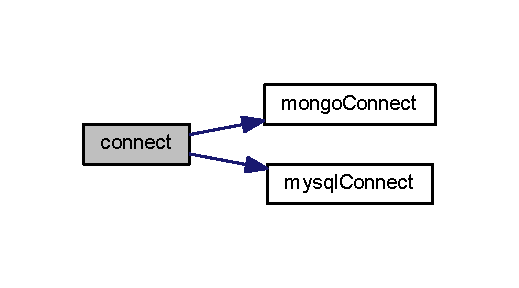
\includegraphics[width=249pt]{class_d_b_connection_a1191ef26fe6381a3bfbd33c0c6f7b9f4_cgraph}
\end{center}
\end{figure}
\mbox{\label{class_d_b_connection_aeb96471cf6f9d9205d22e8b17c2277c3}} 
\index{D\+B\+Connection@{D\+B\+Connection}!connection@{connection}}
\index{connection@{connection}!D\+B\+Connection@{D\+B\+Connection}}
\subsubsection{connection()}
{\footnotesize\ttfamily static connection (\begin{DoxyParamCaption}\item[{string}]{\$db }\end{DoxyParamCaption})\hspace{0.3cm}{\ttfamily [static]}}

Attempts to retrieve a database connection or create one if it has not been extablished yet. \begin{DoxyReturn}{Returns}
Returns a database connection object which may vary from database to database. For older and commonly used databases, {\tt P\+DO} is used when ever possible. For Mongo\+DB, a {\tt } is returned. Null is returned if database credentials are not found or connection establishing fails. 
\end{DoxyReturn}

\begin{DoxyCode}
56                                                    \{
57         $obj = self::obj ();
58         \textcolor{keywordflow}{if} (isset ($obj->connections [$db])) \{
59             \textcolor{keywordflow}{return} $obj->connect ($obj->connections  [$db]);
60         \} \textcolor{keywordflow}{return} null;
61     \}
\end{DoxyCode}
Here is the caller graph for this function\+:
\nopagebreak
\begin{figure}[H]
\begin{center}
\leavevmode
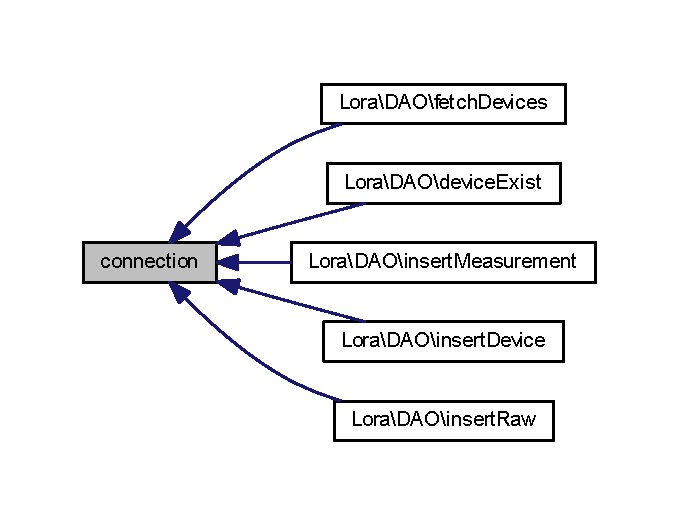
\includegraphics[width=326pt]{class_d_b_connection_aeb96471cf6f9d9205d22e8b17c2277c3_icgraph}
\end{center}
\end{figure}
\mbox{\label{class_d_b_connection_a4db4ce6ff1cf378867220c6694b8bc05}} 
\index{D\+B\+Connection@{D\+B\+Connection}!mongo\+Connect@{mongo\+Connect}}
\index{mongo\+Connect@{mongo\+Connect}!D\+B\+Connection@{D\+B\+Connection}}
\subsubsection{mongo\+Connect()}
{\footnotesize\ttfamily mongo\+Connect (\begin{DoxyParamCaption}\item[{\&}]{\$db }\end{DoxyParamCaption})\hspace{0.3cm}{\ttfamily [private]}}

Connect to a Mongo\+DB -\/database. 
\begin{DoxyCode}
84                                          \{
85         \textcolor{comment}{// 'user' => isset ($db ['user']) ? $db ['user'] : '',}
86         \textcolor{comment}{// 'pass' => isset ($db ['pass']) ? $db ['pass'] : '',}
87         \textcolor{keywordflow}{return} $db [\textcolor{stringliteral}{'connection'}] = new \(\backslash\)MongoDB\(\backslash\)Driver\(\backslash\)Manager (\textcolor{stringliteral}{"mongodb://\{$db ['host']\}:\{$db ['port']\}"})
      ;
88     \}
\end{DoxyCode}
Here is the caller graph for this function\+:
\nopagebreak
\begin{figure}[H]
\begin{center}
\leavevmode
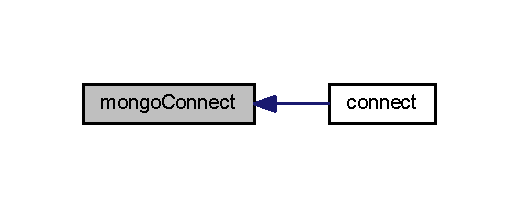
\includegraphics[width=249pt]{class_d_b_connection_a4db4ce6ff1cf378867220c6694b8bc05_icgraph}
\end{center}
\end{figure}
\mbox{\label{class_d_b_connection_ab7140b0e933334f00374b6675c60ffaf}} 
\index{D\+B\+Connection@{D\+B\+Connection}!mysql\+Connect@{mysql\+Connect}}
\index{mysql\+Connect@{mysql\+Connect}!D\+B\+Connection@{D\+B\+Connection}}
\subsubsection{mysql\+Connect()}
{\footnotesize\ttfamily mysql\+Connect (\begin{DoxyParamCaption}\item[{\&}]{\$db }\end{DoxyParamCaption})\hspace{0.3cm}{\ttfamily [private]}}

Connect to a My\+S\+QL -\/database. 
\begin{DoxyCode}
93                                          \{
94         $pdo = null;
95         \textcolor{keywordflow}{try} \{
96             $pdo = \textcolor{keyword}{new} PDO (\textcolor{stringliteral}{"mysql:host=\{$db ['host']\};dbname=\{$db ['database']\};port=\{$db ['port']\}"}, $db 
      [\textcolor{stringliteral}{'user'}], $db [\textcolor{stringliteral}{'password'}]);
97             $pdo->setAttribute (PDO::ATTR\_STRINGIFY\_FETCHES, \textcolor{keyword}{false});
98             $pdo->setAttribute (PDO::ATTR\_EMULATE\_PREPARES, \textcolor{keyword}{false});
99             $pdo->setAttribute (PDO::ATTR\_ERRMODE, PDO::ERRMODE\_EXCEPTION);
100         \} \textcolor{keywordflow}{catch} (PDOException $e) \{
101             \textcolor{comment}{// $pdo->errorCode () === '00000' => success}
102             \textcolor{comment}{// echo 'Connection failed: ' . $e->getMessage();}
103             $pdo = null;
104         \} \textcolor{keywordflow}{return} $db [\textcolor{stringliteral}{'connection'}] = $pdo;
105     \}
\end{DoxyCode}
Here is the caller graph for this function\+:
\nopagebreak
\begin{figure}[H]
\begin{center}
\leavevmode
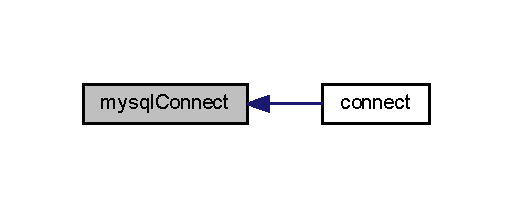
\includegraphics[width=246pt]{class_d_b_connection_ab7140b0e933334f00374b6675c60ffaf_icgraph}
\end{center}
\end{figure}
\mbox{\label{class_d_b_connection_a2b99fe8f4ca4b64909ce7b499e71dfb6}} 
\index{D\+B\+Connection@{D\+B\+Connection}!obj@{obj}}
\index{obj@{obj}!D\+B\+Connection@{D\+B\+Connection}}
\subsubsection{obj()}
{\footnotesize\ttfamily static obj (\begin{DoxyParamCaption}{ }\end{DoxyParamCaption})\hspace{0.3cm}{\ttfamily [static]}, {\ttfamily [private]}}

\begin{DoxyReturn}{Returns}
Returns a singleton instance of this class which is created upon first call to this method. 
\end{DoxyReturn}

\begin{DoxyCode}
45                                    \{
46         \textcolor{keywordflow}{return} self::$instance ?? (self::$instance = \textcolor{keyword}{new} DBConnection ());
47     \}
\end{DoxyCode}


\subsection{Field Documentation}
\mbox{\label{class_d_b_connection_a8d01870fbfcf9232c0e94c50a7142331}} 
\index{D\+B\+Connection@{D\+B\+Connection}!\$connections@{\$connections}}
\index{\$connections@{\$connections}!D\+B\+Connection@{D\+B\+Connection}}
\subsubsection{\$connections}
{\footnotesize\ttfamily \$connections\hspace{0.3cm}{\ttfamily [private]}}

{\bfseries Initial value\+:}
\begin{DoxyCode}
= [
                \textcolor{stringliteral}{'measurements'} => [
                    \textcolor{stringliteral}{"type"}          => DBConnection::MONGO
\end{DoxyCode}


\$connections holds all available database credentials. 

\mbox{\label{class_d_b_connection_a832ddc04754e8a43d4f3c6165b1294a7}} 
\index{D\+B\+Connection@{D\+B\+Connection}!host@{host}}
\index{host@{host}!D\+B\+Connection@{D\+B\+Connection}}
\subsubsection{host}
{\footnotesize\ttfamily host}

{\bfseries Initial value\+:}
\begin{DoxyCode}
=> \textcolor{stringliteral}{"localhost"},
                    \textcolor{stringliteral}{"port"}          => \textcolor{stringliteral}{"27017"},
                    \textcolor{stringliteral}{"connection"}    => null
                ]
                
            ]
\end{DoxyCode}


The documentation for this class was generated from the following file\+:\begin{DoxyCompactItemize}
\item 
lora/dbconnection.\+php\end{DoxyCompactItemize}

\hypertarget{class_lora_1_1_api_1_1echo_server}{}\section{echo\+Server Class Reference}
\label{class_lora_1_1_api_1_1echo_server}\index{echo\+Server@{echo\+Server}}


Inheritance diagram for echo\+Server\+:
% FIG 0


Collaboration diagram for echo\+Server\+:
% FIG 1
\subsection*{Public Member Functions}
\begin{DoxyCompactItemize}
\item 
\mbox{\Hypertarget{class_lora_1_1_api_1_1echo_server_a473114c92843eda7de537f42ffde8913}\label{class_lora_1_1_api_1_1echo_server_a473114c92843eda7de537f42ffde8913}} 
{\bfseries broadcast} (string \$msg)
\end{DoxyCompactItemize}
\subsection*{Protected Member Functions}
\begin{DoxyCompactItemize}
\item 
\mbox{\Hypertarget{class_lora_1_1_api_1_1echo_server_a805b6933fa0b69978e35fe94f3884de7}\label{class_lora_1_1_api_1_1echo_server_a805b6933fa0b69978e35fe94f3884de7}} 
{\bfseries process} (\$user, \$message)
\item 
\mbox{\Hypertarget{class_lora_1_1_api_1_1echo_server_a3e89014762456a67edbe843811c78736}\label{class_lora_1_1_api_1_1echo_server_a3e89014762456a67edbe843811c78736}} 
{\bfseries connected} (\$user)
\item 
\mbox{\Hypertarget{class_lora_1_1_api_1_1echo_server_aaf6375ec8ee41584a5adcf3d85d73018}\label{class_lora_1_1_api_1_1echo_server_aaf6375ec8ee41584a5adcf3d85d73018}} 
{\bfseries closed} (\$user)
\end{DoxyCompactItemize}


The documentation for this class was generated from the following file\+:\begin{DoxyCompactItemize}
\item 
servers/webserver/server/api/socket/socket.\+php\end{DoxyCompactItemize}

\section{Html\+Lib Class Reference}
\label{class_html_1_1_html_lib}\index{Html\+Lib@{Html\+Lib}}
\subsection*{Static Public Member Functions}
\begin{DoxyCompactItemize}
\item 
static \textbf{ attr\+Name\+Check} (string \$name)
\end{DoxyCompactItemize}


\subsection{Detailed Description}
An H\+T\+ML library class to contain various H\+T\+ML related utility functions. 

\subsection{Member Function Documentation}
\mbox{\label{class_html_1_1_html_lib_a53ec3d81bbf119ac8be017abed712c32}} 
\index{Html\+::\+Html\+Lib@{Html\+::\+Html\+Lib}!attr\+Name\+Check@{attr\+Name\+Check}}
\index{attr\+Name\+Check@{attr\+Name\+Check}!Html\+::\+Html\+Lib@{Html\+::\+Html\+Lib}}
\subsubsection{attr\+Name\+Check()}
{\footnotesize\ttfamily static attr\+Name\+Check (\begin{DoxyParamCaption}\item[{string}]{\$name }\end{DoxyParamCaption})\hspace{0.3cm}{\ttfamily [static]}}

Ensures validity of an H\+T\+ML attribute name. 
\begin{DoxyCode}
14                                                         \{
15         \textcolor{keywordflow}{return} preg\_match (\textcolor{stringliteral}{'/^[a-z-]+$/'}, $name) === 1;
16     \}
\end{DoxyCode}


The documentation for this class was generated from the following file\+:\begin{DoxyCompactItemize}
\item 
servers/webserver/server/util/htmllib.\+php\end{DoxyCompactItemize}

\hypertarget{class_html_1_1_html_tag}{}\section{Html\+Tag Class Reference}
\label{class_html_1_1_html_tag}\index{Html\+Tag@{Html\+Tag}}


Inheritance diagram for Html\+Tag\+:
% FIG 0
\subsection*{Public Member Functions}
\begin{DoxyCompactItemize}
\item 
\hyperlink{class_html_1_1_html_tag_ab2972fb46953f5babb049c5f1c664512}{tag} ()
\item 
\hyperlink{class_html_1_1_html_tag_a80b8713959c19499c9a177d883a5a96b}{set\+Attr} (string \$name, \$value)
\item 
\hyperlink{class_html_1_1_html_tag_a75ef0c456595eaa6a574c438803fb072}{attrs} (bool \$string=false)
\item 
\hyperlink{class_html_1_1_html_tag_a43374e600f552e0a9308ab96b1964aba}{print} ()
\end{DoxyCompactItemize}
\subsection*{Data Fields}
\begin{DoxyCompactItemize}
\item 
\mbox{\Hypertarget{class_html_1_1_html_tag_af4cf24d99d068a1aefe99caf8dd8a458}\label{class_html_1_1_html_tag_af4cf24d99d068a1aefe99caf8dd8a458}} 
{\bfseries \$attrs} = \mbox{[}$\,$\mbox{]}
\item 
\mbox{\Hypertarget{class_html_1_1_html_tag_a4212f1eca3e4faf764728d56bc13dfd3}\label{class_html_1_1_html_tag_a4212f1eca3e4faf764728d56bc13dfd3}} 
{\bfseries \$classes} = \mbox{[}$\,$\mbox{]}
\end{DoxyCompactItemize}
\subsection*{Protected Attributes}
\begin{DoxyCompactItemize}
\item 
\mbox{\Hypertarget{class_html_1_1_html_tag_a81d5015d41ed8ec66e9db8cdc5db9555}\label{class_html_1_1_html_tag_a81d5015d41ed8ec66e9db8cdc5db9555}} 
{\bfseries \$tag} = \textquotesingle{}\textquotesingle{}
\end{DoxyCompactItemize}


\subsection{Detailed Description}
An abstract base class for representing H\+T\+ML tags. Makes certain things easier when working with template engines such as printing comples hyperlinks easily. \begin{DoxyRefDesc}{Todo}
\item[\hyperlink{todo__todo000012}{Todo}]Needs improvements and has to better comply H\+T\+ML structure.
\begin{DoxyItemize}
\item Add an array for inner contents.
\item Add utility funtions for certain commonly used attributes such as id and class.
\item A better approach to creating an H\+T\+ML management system would be to write specialized attribute classes instead of tag classes. 
\end{DoxyItemize}\end{DoxyRefDesc}


\subsection{Member Function Documentation}
\mbox{\Hypertarget{class_html_1_1_html_tag_a75ef0c456595eaa6a574c438803fb072}\label{class_html_1_1_html_tag_a75ef0c456595eaa6a574c438803fb072}} 
\index{Html\+::\+Html\+Tag@{Html\+::\+Html\+Tag}!attrs@{attrs}}
\index{attrs@{attrs}!Html\+::\+Html\+Tag@{Html\+::\+Html\+Tag}}
\subsubsection{\texorpdfstring{attrs()}{attrs()}}
{\footnotesize\ttfamily attrs (\begin{DoxyParamCaption}\item[{bool}]{\$string = {\ttfamily false} }\end{DoxyParamCaption})}

Returns this Html\+Tags attributes in either string or array form. 
\begin{DoxyParams}{Parameters}
{\em \$string} & A boolean value to determine the return value of this method. \\
\hline
\end{DoxyParams}
\begin{DoxyReturn}{Returns}
Returns attributes as an array if \$string is false and as a string if it is true. 
\end{DoxyReturn}

\begin{DoxyCode}
56                                                  \{
57         \textcolor{keywordflow}{if} ($string) \{
58             $attrs = \textcolor{stringliteral}{''};
59             \textcolor{keywordflow}{foreach} ($this->\hyperlink{class_html_1_1_html_tag_a75ef0c456595eaa6a574c438803fb072}{attrs} as $name => $value) \{
60                 $attrs .= \textcolor{stringliteral}{"$\{name\}=\(\backslash\)"$\{value\}\(\backslash\)" "};
61             \} \textcolor{keywordflow}{return} substr ($attrs, 0, -1);
62         \} \textcolor{keywordflow}{return} $this->attrs;
63     \}
\end{DoxyCode}
\mbox{\Hypertarget{class_html_1_1_html_tag_a43374e600f552e0a9308ab96b1964aba}\label{class_html_1_1_html_tag_a43374e600f552e0a9308ab96b1964aba}} 
\index{Html\+::\+Html\+Tag@{Html\+::\+Html\+Tag}!print@{print}}
\index{print@{print}!Html\+::\+Html\+Tag@{Html\+::\+Html\+Tag}}
\subsubsection{\texorpdfstring{print()}{print()}}
{\footnotesize\ttfamily print (\begin{DoxyParamCaption}{ }\end{DoxyParamCaption})\hspace{0.3cm}{\ttfamily [abstract]}}

A method to print this tag instance as a string. \mbox{\Hypertarget{class_html_1_1_html_tag_a80b8713959c19499c9a177d883a5a96b}\label{class_html_1_1_html_tag_a80b8713959c19499c9a177d883a5a96b}} 
\index{Html\+::\+Html\+Tag@{Html\+::\+Html\+Tag}!set\+Attr@{set\+Attr}}
\index{set\+Attr@{set\+Attr}!Html\+::\+Html\+Tag@{Html\+::\+Html\+Tag}}
\subsubsection{\texorpdfstring{set\+Attr()}{setAttr()}}
{\footnotesize\ttfamily set\+Attr (\begin{DoxyParamCaption}\item[{string}]{\$name,  }\item[{}]{\$value }\end{DoxyParamCaption})}

Checks attribute name and sets it for this \hyperlink{class_html_1_1_html_tag}{Html\+Tag} if found valid. 
\begin{DoxyParams}{Parameters}
{\em \$name} & Name of the attribute. \\
\hline
{\em \$value} & Value of the attribute. \\
\hline
\end{DoxyParams}
\begin{DoxyReturn}{Returns}
Returns this current instance. 
\end{DoxyReturn}

\begin{DoxyCode}
44                                                    \{
45         \textcolor{keywordflow}{if} (\hyperlink{class_html_1_1_html_lib_a53ec3d81bbf119ac8be017abed712c32}{HtmlLib::attrNameCheck} ($name)) \{
46             $this->\hyperlink{class_html_1_1_html_tag_a75ef0c456595eaa6a574c438803fb072}{attrs} [$name] = $value;
47         \}
48         \textcolor{keywordflow}{return} $this;
49     \}
\end{DoxyCode}
\mbox{\Hypertarget{class_html_1_1_html_tag_ab2972fb46953f5babb049c5f1c664512}\label{class_html_1_1_html_tag_ab2972fb46953f5babb049c5f1c664512}} 
\index{Html\+::\+Html\+Tag@{Html\+::\+Html\+Tag}!tag@{tag}}
\index{tag@{tag}!Html\+::\+Html\+Tag@{Html\+::\+Html\+Tag}}
\subsubsection{\texorpdfstring{tag()}{tag()}}
{\footnotesize\ttfamily tag (\begin{DoxyParamCaption}{ }\end{DoxyParamCaption})}

\begin{DoxyReturn}{Returns}
Returns tag name of this \hyperlink{class_html_1_1_html_tag}{Html\+Tag}. 
\end{DoxyReturn}

\begin{DoxyCode}
34                            \{
35         \textcolor{keywordflow}{return} $this->tag;
36     \}
\end{DoxyCode}


The documentation for this class was generated from the following file\+:\begin{DoxyCompactItemize}
\item 
servers/webserver/server/util/htmltag.\+php\end{DoxyCompactItemize}

\hypertarget{class_internal_m_s_g}{}\section{Internal\+M\+SG Class Reference}
\label{class_internal_m_s_g}\index{Internal\+M\+SG@{Internal\+M\+SG}}
\subsection*{Static Public Member Functions}
\begin{DoxyCompactItemize}
\item 
static \hyperlink{class_internal_m_s_g_ae3b91a7baffc1bef8eaeb4a5bcca65f0}{compose\+Msg} (int \$command, array \$message)
\item 
static \hyperlink{class_internal_m_s_g_ab515acd10479df5ff64b2584a2f8fa9d}{decompose\+Msg} (string \$msg)
\end{DoxyCompactItemize}


\subsection{Detailed Description}
A messaging utility class used to unify and manage internal messaging within various server subsystems. 

\subsection{Member Function Documentation}
\mbox{\Hypertarget{class_internal_m_s_g_ae3b91a7baffc1bef8eaeb4a5bcca65f0}\label{class_internal_m_s_g_ae3b91a7baffc1bef8eaeb4a5bcca65f0}} 
\index{Internal\+M\+SG@{Internal\+M\+SG}!compose\+Msg@{compose\+Msg}}
\index{compose\+Msg@{compose\+Msg}!Internal\+M\+SG@{Internal\+M\+SG}}
\subsubsection{\texorpdfstring{compose\+Msg()}{composeMsg()}}
{\footnotesize\ttfamily static compose\+Msg (\begin{DoxyParamCaption}\item[{int}]{\$command,  }\item[{array}]{\$message }\end{DoxyParamCaption})\hspace{0.3cm}{\ttfamily [static]}}

Composes an encoded message used for internal messaging within the server complex. 
\begin{DoxyParams}{Parameters}
{\em \$command} & One of the Command constants. \\
\hline
{\em \$message} & An array containing relevant data for this command. \\
\hline
\end{DoxyParams}
\begin{DoxyReturn}{Returns}
Returns a formatted message string. 
\end{DoxyReturn}

\begin{DoxyCode}
17                                                                      : \textcolor{keywordtype}{string} \{
18         \textcolor{keywordflow}{return} \textcolor{stringliteral}{"$command:"}.json\_encode ($message);
19     \}
\end{DoxyCode}
\mbox{\Hypertarget{class_internal_m_s_g_ab515acd10479df5ff64b2584a2f8fa9d}\label{class_internal_m_s_g_ab515acd10479df5ff64b2584a2f8fa9d}} 
\index{Internal\+M\+SG@{Internal\+M\+SG}!decompose\+Msg@{decompose\+Msg}}
\index{decompose\+Msg@{decompose\+Msg}!Internal\+M\+SG@{Internal\+M\+SG}}
\subsubsection{\texorpdfstring{decompose\+Msg()}{decomposeMsg()}}
{\footnotesize\ttfamily static decompose\+Msg (\begin{DoxyParamCaption}\item[{string}]{\$msg }\end{DoxyParamCaption})\hspace{0.3cm}{\ttfamily [static]}}

Decomposes an encoded message and decodes it into useable component. If the message cannot be decoded, an invalid message array is returned with Command\+::\+I\+N\+V\+A\+L\+ID in its 0 index and nothing in 1 index. 
\begin{DoxyParams}{Parameters}
{\em \$msg} & Message to decode. \\
\hline
\end{DoxyParams}
\begin{DoxyReturn}{Returns}
Returns an array containing the decoded message. 0 index holds the Command -\/value and 1 index the decoded message. 
\end{DoxyReturn}

\begin{DoxyCode}
28                                                       : array \{
29         \textcolor{keywordflow}{if} (($pos = strpos ($message, \textcolor{charliteral}{':'})) === \textcolor{keyword}{false} || ($command = 
      \hyperlink{class_data_lib_a60cb59e0d64619154c155046e6e4ca66}{DataLib::isInt} (substr ($message, 0, $pos))) === \textcolor{keyword}{false} || !Command::isCommand ($command)) \{
30             \textcolor{keywordflow}{return} [ Command::INVALID ];
31         \}
32         \textcolor{keywordflow}{return} [
33             $command,
34             json\_decode (substr ($message, $pos + 1))
35         ];
36     \}
\end{DoxyCode}
Here is the call graph for this function\+:
% FIG 0


The documentation for this class was generated from the following file\+:\begin{DoxyCompactItemize}
\item 
lora/internalmsg.\+php\end{DoxyCompactItemize}

\section{Lib Class Reference}
\label{class_lib}\index{Lib@{Lib}}
\subsection*{Public Member Functions}
\begin{DoxyCompactItemize}
\item 
\textbf{ array\+To\+String} (array \$data, string \$delim, bool \$keyed=false, string \$glue=\textquotesingle{}\textquotesingle{})
\end{DoxyCompactItemize}
\subsection*{Static Public Member Functions}
\begin{DoxyCompactItemize}
\item 
static \textbf{ dump} (\$val, bool \$return=false)
\item 
static \textbf{ check\+Extension} (string \$file\+Name, string \$extension)
\end{DoxyCompactItemize}


\subsection{Detailed Description}
A class to contain more or less universal library functions which can be used in any project. 

\subsection{Member Function Documentation}
\mbox{\label{class_lib_a792f12586807e89f69e34b7392d6417d}} 
\index{Lib@{Lib}!array\+To\+String@{array\+To\+String}}
\index{array\+To\+String@{array\+To\+String}!Lib@{Lib}}
\subsubsection{array\+To\+String()}
{\footnotesize\ttfamily array\+To\+String (\begin{DoxyParamCaption}\item[{array}]{\$data,  }\item[{string}]{\$delim,  }\item[{bool}]{\$keyed = {\ttfamily false},  }\item[{string}]{\$glue = {\ttfamily \textquotesingle{}\textquotesingle{}} }\end{DoxyParamCaption})}

Builds a string from an array of data. Only works with one dimensional arrays and scalar types. 
\begin{DoxyParams}{Parameters}
{\em \$data} & An array of data to be concatenated into a string. \\
\hline
{\em \$delim} & Delimiter string added between values. \\
\hline
{\em \$keyed} & A boolean value to dictate if array keys should be included in the final string. \\
\hline
{\em \$glue} & A string to be added between key and value pairs. Used only if keyed is true. \\
\hline
\end{DoxyParams}

\begin{DoxyCode}
35                                                                                                        \{
36         $string = \textcolor{stringliteral}{''};
37         \textcolor{keywordflow}{if} ($keyed) \{
38             \textcolor{keywordflow}{foreach} ($data as $key => $value) \{
39                 \textcolor{keywordflow}{if} (empty ($value)) \{
40                     $string .= $key.$delim;
41                 \} \textcolor{keywordflow}{else} \{
42                     $string .= $key.$glue.$value.$delim;
43                 \}
44             \}
45         \} \textcolor{keywordflow}{else} \{
46             \textcolor{keywordflow}{foreach} ($data as $value) \{
47                 $string .= $value.$delim;
48             \}
49         \} \textcolor{keywordflow}{return} substr ($string, 0, -strlen ($delim));
50     \}
\end{DoxyCode}
Here is the caller graph for this function\+:\nopagebreak
\begin{figure}[H]
\begin{center}
\leavevmode
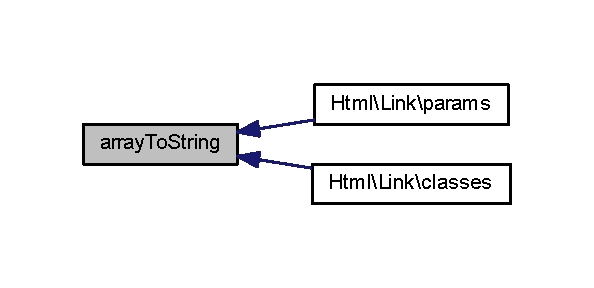
\includegraphics[width=285pt]{class_lib_a792f12586807e89f69e34b7392d6417d_icgraph}
\end{center}
\end{figure}
\mbox{\label{class_lib_ab5fbdf394f09fcef4dcea271c344cb65}} 
\index{Lib@{Lib}!check\+Extension@{check\+Extension}}
\index{check\+Extension@{check\+Extension}!Lib@{Lib}}
\subsubsection{check\+Extension()}
{\footnotesize\ttfamily static check\+Extension (\begin{DoxyParamCaption}\item[{string}]{\$file\+Name,  }\item[{string}]{\$extension }\end{DoxyParamCaption})\hspace{0.3cm}{\ttfamily [static]}}

A function to check if a file name has given extension in it and adds one if it is not found. 
\begin{DoxyParams}{Parameters}
{\em \$file} & A file name to be checked for extension. \\
\hline
{\em \$extension} & An extension to check against and to add if not found. \\
\hline
\end{DoxyParams}

\begin{DoxyCode}
57                                                                                 : \textcolor{keywordtype}{string} \{
58         \textcolor{keywordflow}{if} (!empty ($fileName) && empty (pathinfo ($fileName, PATHINFO\_EXTENSION))) \{
59             \textcolor{keywordflow}{return} \textcolor{stringliteral}{"\{$fileName\}.\{$extension\}"};;
60         \} \textcolor{keywordflow}{return} $fileName;
61     \}
\end{DoxyCode}
Here is the caller graph for this function\+:\nopagebreak
\begin{figure}[H]
\begin{center}
\leavevmode
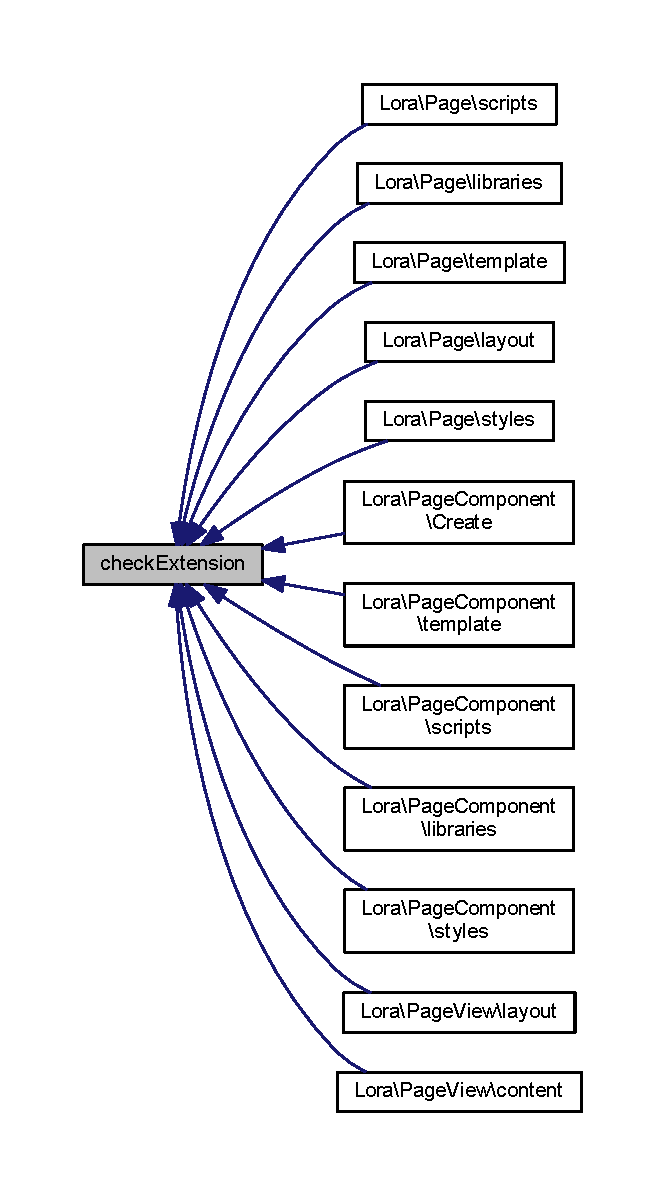
\includegraphics[height=550pt]{class_lib_ab5fbdf394f09fcef4dcea271c344cb65_icgraph}
\end{center}
\end{figure}
\mbox{\label{class_lib_a29c2b6b4cde743c320b8a9e30056a6dd}} 
\index{Lib@{Lib}!dump@{dump}}
\index{dump@{dump}!Lib@{Lib}}
\subsubsection{dump()}
{\footnotesize\ttfamily static dump (\begin{DoxyParamCaption}\item[{}]{\$val,  }\item[{bool}]{\$return = {\ttfamily false} }\end{DoxyParamCaption})\hspace{0.3cm}{\ttfamily [static]}}

Pretty prints the given value as H\+T\+ML, wrapped in pre -\/tags. Optionally, returns the pretty printed data instead of appending to the out buffer with echo. 
\begin{DoxyParams}{Parameters}
{\em \$val} & Value to be printed. \\
\hline
{\em \$return} & An optional boolean value defaulting to false to choose if the pretty printed value should be returned. \\
\hline
\end{DoxyParams}

\begin{DoxyCode}
20                                                              \{
21         $val = \textcolor{stringliteral}{'<pre>'}.print\_r ($val, \textcolor{keyword}{true}).\textcolor{stringliteral}{'</pre>'};
22         \textcolor{keywordflow}{if} ($return) \{
23             \textcolor{keywordflow}{return} $val;
24         \}
25         echo $val;
26     \}
\end{DoxyCode}


The documentation for this class was generated from the following file\+:\begin{DoxyCompactItemize}
\item 
lora/util/lib.\+php\end{DoxyCompactItemize}

\hypertarget{class_html_1_1_link}{}\section{Link Class Reference}
\label{class_html_1_1_link}\index{Link@{Link}}


Inheritance diagram for Link\+:
% FIG 0


Collaboration diagram for Link\+:
% FIG 1
\subsection*{Public Member Functions}
\begin{DoxyCompactItemize}
\item 
\mbox{\Hypertarget{class_html_1_1_link_af17abe69a60a77b0891506c3bbc208ec}\label{class_html_1_1_link_af17abe69a60a77b0891506c3bbc208ec}} 
{\bfseries \+\_\+\+\_\+construct} (string \$\hyperlink{class_html_1_1_link_ab7fdada65bce8f1069e5cbbbf532ca8f}{text}=\textquotesingle{}\textquotesingle{}, string \$ref=\textquotesingle{}\textquotesingle{}, array \$\hyperlink{class_html_1_1_link_a781949bb79e8bfc4148fcc40c6b9fb3b}{params}=\mbox{[}$\,$\mbox{]}, array \$\hyperlink{class_html_1_1_html_tag_a75ef0c456595eaa6a574c438803fb072}{attrs}=\mbox{[}$\,$\mbox{]}, array \$\hyperlink{class_html_1_1_link_af6ac36c4e10b38c61aa0b45fa736bfc4}{classes}=\mbox{[}$\,$\mbox{]})
\item 
\hyperlink{class_html_1_1_link_a43374e600f552e0a9308ab96b1964aba}{print} ()
\item 
\hyperlink{class_html_1_1_link_acca9a5a3248aa2412373b1fe3a7e2a01}{href} (string \$ref=\textquotesingle{}\textquotesingle{})
\item 
\hyperlink{class_html_1_1_link_ab7fdada65bce8f1069e5cbbbf532ca8f}{text} (string \$text=\textquotesingle{}\textquotesingle{})
\item 
\hyperlink{class_html_1_1_link_a3a12152c8947fb47e6833a6e1164c730}{set\+Param} (string \$name, \$value)
\item 
\hyperlink{class_html_1_1_link_a781949bb79e8bfc4148fcc40c6b9fb3b}{params} (bool \$string=false)
\item 
\hyperlink{class_html_1_1_link_a45453935ed565c45623fb7b8b8c9810b}{add\+Class} (string \$class)
\item 
\hyperlink{class_html_1_1_link_af6ac36c4e10b38c61aa0b45fa736bfc4}{classes} (bool \$string=false)
\end{DoxyCompactItemize}
\subsection*{Data Fields}
\begin{DoxyCompactItemize}
\item 
\mbox{\Hypertarget{class_html_1_1_link_a8f8757e72f75875c4520aa66624dfae2}\label{class_html_1_1_link_a8f8757e72f75875c4520aa66624dfae2}} 
{\bfseries \$refs} = \textquotesingle{}\textquotesingle{}
\item 
\mbox{\Hypertarget{class_html_1_1_link_afe68e6fbe7acfbffc0af0c84a1996466}\label{class_html_1_1_link_afe68e6fbe7acfbffc0af0c84a1996466}} 
{\bfseries \$params} = \mbox{[}$\,$\mbox{]}
\end{DoxyCompactItemize}
\subsection*{Private Attributes}
\begin{DoxyCompactItemize}
\item 
\mbox{\Hypertarget{class_html_1_1_link_adf95f30eaafccead90ab5e2cdb55e9b9}\label{class_html_1_1_link_adf95f30eaafccead90ab5e2cdb55e9b9}} 
{\bfseries \$text} = \textquotesingle{}\textquotesingle{}
\end{DoxyCompactItemize}
\subsection*{Additional Inherited Members}


\subsection{Detailed Description}
A class to represent an H\+T\+ML hyperlink. Makes creating and managing hyperlinks in twig easier by a magnitude. Can be used as an anchor tag aswell. 

\subsection{Member Function Documentation}
\mbox{\Hypertarget{class_html_1_1_link_a45453935ed565c45623fb7b8b8c9810b}\label{class_html_1_1_link_a45453935ed565c45623fb7b8b8c9810b}} 
\index{Html\+::\+Link@{Html\+::\+Link}!add\+Class@{add\+Class}}
\index{add\+Class@{add\+Class}!Html\+::\+Link@{Html\+::\+Link}}
\subsubsection{\texorpdfstring{add\+Class()}{addClass()}}
{\footnotesize\ttfamily add\+Class (\begin{DoxyParamCaption}\item[{string}]{\$class }\end{DoxyParamCaption})}

Adds a new css class to this \hyperlink{class_html_1_1_html_tag}{Html\+Tag}. 
\begin{DoxyParams}{Parameters}
{\em \$class} & Name of the css class to be added. \\
\hline
\end{DoxyParams}
\begin{DoxyReturn}{Returns}
Returns this \hyperlink{class_html_1_1_html_tag}{Html\+Tag}. 
\end{DoxyReturn}

\begin{DoxyCode}
86                                              \{
87         $this->\hyperlink{class_html_1_1_link_af6ac36c4e10b38c61aa0b45fa736bfc4}{classes} [] = $class;
88         \textcolor{keywordflow}{return} $this;
89     \}
\end{DoxyCode}
\mbox{\Hypertarget{class_html_1_1_link_af6ac36c4e10b38c61aa0b45fa736bfc4}\label{class_html_1_1_link_af6ac36c4e10b38c61aa0b45fa736bfc4}} 
\index{Html\+::\+Link@{Html\+::\+Link}!classes@{classes}}
\index{classes@{classes}!Html\+::\+Link@{Html\+::\+Link}}
\subsubsection{\texorpdfstring{classes()}{classes()}}
{\footnotesize\ttfamily classes (\begin{DoxyParamCaption}\item[{bool}]{\$string = {\ttfamily false} }\end{DoxyParamCaption})}

Returns all classes this \hyperlink{class_html_1_1_html_tag}{Html\+Tag} has as a string or an array. 
\begin{DoxyParams}{Parameters}
{\em \$string} & A boolean value to determine the reutrn value of this method. \\
\hline
\end{DoxyParams}
\begin{DoxyReturn}{Returns}
Returns an array of parameter values if \$string is false and a string presentation of them if it is true. 
\end{DoxyReturn}

\begin{DoxyCode}
96                                                    \{
97         \textcolor{keywordflow}{return} $string ? \hyperlink{class_lib_a792f12586807e89f69e34b7392d6417d}{\(\backslash\)Lib::arrayToString} ($this->\hyperlink{class_html_1_1_link_af6ac36c4e10b38c61aa0b45fa736bfc4}{classes}, \textcolor{charliteral}{' '}) : $this->
      \hyperlink{class_html_1_1_link_af6ac36c4e10b38c61aa0b45fa736bfc4}{classes};
98     \}
\end{DoxyCode}
Here is the call graph for this function\+:
% FIG 2
\mbox{\Hypertarget{class_html_1_1_link_acca9a5a3248aa2412373b1fe3a7e2a01}\label{class_html_1_1_link_acca9a5a3248aa2412373b1fe3a7e2a01}} 
\index{Html\+::\+Link@{Html\+::\+Link}!href@{href}}
\index{href@{href}!Html\+::\+Link@{Html\+::\+Link}}
\subsubsection{\texorpdfstring{href()}{href()}}
{\footnotesize\ttfamily href (\begin{DoxyParamCaption}\item[{string}]{\$ref = {\ttfamily \textquotesingle{}\textquotesingle{}} }\end{DoxyParamCaption})}

Set or get the target location of this \hyperlink{class_html_1_1_link}{Link}. If \$ref is empty, this method returns a fully constructed hyper reference string. 
\begin{DoxyParams}{Parameters}
{\em \$ref} & Target location or an anchor. \\
\hline
\end{DoxyParams}
\begin{DoxyReturn}{Returns}
Returns this \hyperlink{class_html_1_1_link}{Link} instance if \$ref is not empty and a string representation of the target if it is empty. 
\end{DoxyReturn}

\begin{DoxyCode}
39                                             \{
40         \textcolor{keywordflow}{if} (empty ($ref)) \{
41             $params = $this->\hyperlink{class_html_1_1_link_a781949bb79e8bfc4148fcc40c6b9fb3b}{params} (\textcolor{keyword}{true});
42             return \(\backslash\)Lora\(\backslash\)Config::get (\textcolor{stringliteral}{'client'}, \textcolor{stringliteral}{'pages'}).\textcolor{stringliteral}{"\{$this->refs\}"}.(!empty ($params) ? \textcolor{stringliteral}{"?$\{params\}"} :
       \textcolor{stringliteral}{''});
43         \}
44         $this->refs = $ref;
45         \textcolor{keywordflow}{return} $this;
46     \}
\end{DoxyCode}
\mbox{\Hypertarget{class_html_1_1_link_a781949bb79e8bfc4148fcc40c6b9fb3b}\label{class_html_1_1_link_a781949bb79e8bfc4148fcc40c6b9fb3b}} 
\index{Html\+::\+Link@{Html\+::\+Link}!params@{params}}
\index{params@{params}!Html\+::\+Link@{Html\+::\+Link}}
\subsubsection{\texorpdfstring{params()}{params()}}
{\footnotesize\ttfamily params (\begin{DoxyParamCaption}\item[{bool}]{\$string = {\ttfamily false} }\end{DoxyParamCaption})}

Returns all the parameters this \hyperlink{class_html_1_1_link}{Link} has as a string or an array. 
\begin{DoxyParams}{Parameters}
{\em \$string} & A boolean value to determine the return value of this method. \\
\hline
\end{DoxyParams}
\begin{DoxyReturn}{Returns}
Returns an array of parameter values if \$string is false and a string presentation of them if it is true. 
\end{DoxyReturn}

\begin{DoxyCode}
77                                                   \{
78         \textcolor{keywordflow}{return} $string ? \hyperlink{class_lib_a792f12586807e89f69e34b7392d6417d}{\(\backslash\)Lib::arrayToString} ($this->\hyperlink{class_html_1_1_link_a781949bb79e8bfc4148fcc40c6b9fb3b}{params}, \textcolor{charliteral}{'&'}, \textcolor{keyword}{true}, \textcolor{charliteral}{'='}) : 
      $this->\hyperlink{class_html_1_1_link_a781949bb79e8bfc4148fcc40c6b9fb3b}{params};
79     \}
\end{DoxyCode}
Here is the call graph for this function\+:
% FIG 3
\mbox{\Hypertarget{class_html_1_1_link_a43374e600f552e0a9308ab96b1964aba}\label{class_html_1_1_link_a43374e600f552e0a9308ab96b1964aba}} 
\index{Html\+::\+Link@{Html\+::\+Link}!print@{print}}
\index{print@{print}!Html\+::\+Link@{Html\+::\+Link}}
\subsubsection{\texorpdfstring{print()}{print()}}
{\footnotesize\ttfamily print (\begin{DoxyParamCaption}{ }\end{DoxyParamCaption})}

Print implementation for H\+T\+ML anchor tag. Overrides \hyperlink{class_html_1_1_html_tag_a43374e600f552e0a9308ab96b1964aba}{Html\+Tag\+::print}. \begin{DoxyReturn}{Returns}
Returns a string representation of an H\+T\+ML link. 
\end{DoxyReturn}

\begin{DoxyCode}
30                              : \textcolor{keywordtype}{string} \{
31         \textcolor{keywordflow}{return} \textcolor{stringliteral}{"<\{$this->tag\} href=\(\backslash\)""}.$this->href ().\textcolor{stringliteral}{"\(\backslash\)" "}.$this->\hyperlink{class_html_1_1_html_tag_a75ef0c456595eaa6a574c438803fb072}{attrs} (\textcolor{keyword}{true}).\textcolor{stringliteral}{"
      >\{$this->text\}</\{$this->tag\}>"};
32     \}
\end{DoxyCode}
\mbox{\Hypertarget{class_html_1_1_link_a3a12152c8947fb47e6833a6e1164c730}\label{class_html_1_1_link_a3a12152c8947fb47e6833a6e1164c730}} 
\index{Html\+::\+Link@{Html\+::\+Link}!set\+Param@{set\+Param}}
\index{set\+Param@{set\+Param}!Html\+::\+Link@{Html\+::\+Link}}
\subsubsection{\texorpdfstring{set\+Param()}{setParam()}}
{\footnotesize\ttfamily set\+Param (\begin{DoxyParamCaption}\item[{string}]{\$name,  }\item[{}]{\$value }\end{DoxyParamCaption})}

Adds a new or overrides an existing hyper link parameter pair. 
\begin{DoxyParams}{Parameters}
{\em \$name} & Name of the paramter. \\
\hline
{\em \$value} & Value of the parameter. \\
\hline
\end{DoxyParams}
\begin{DoxyReturn}{Returns}
Returns this \hyperlink{class_html_1_1_link}{Link} object. 
\end{DoxyReturn}

\begin{DoxyCode}
67                                                     : Link \{
68         $this->\hyperlink{class_html_1_1_link_a781949bb79e8bfc4148fcc40c6b9fb3b}{params} [$name] = $value;
69         \textcolor{keywordflow}{return} $this;
70     \}
\end{DoxyCode}
\mbox{\Hypertarget{class_html_1_1_link_ab7fdada65bce8f1069e5cbbbf532ca8f}\label{class_html_1_1_link_ab7fdada65bce8f1069e5cbbbf532ca8f}} 
\index{Html\+::\+Link@{Html\+::\+Link}!text@{text}}
\index{text@{text}!Html\+::\+Link@{Html\+::\+Link}}
\subsubsection{\texorpdfstring{text()}{text()}}
{\footnotesize\ttfamily text (\begin{DoxyParamCaption}\item[{string}]{\$text = {\ttfamily \textquotesingle{}\textquotesingle{}} }\end{DoxyParamCaption})}

Sets or gets the inner text of this \hyperlink{class_html_1_1_link}{Link}. If \$text is empty, current Link\+::\$text is returned. If not, \$text replaces current Link\+::\$text. 
\begin{DoxyParams}{Parameters}
{\em \$text} & An optional new text for this \hyperlink{class_html_1_1_link}{Link}. \\
\hline
\end{DoxyParams}
\begin{DoxyReturn}{Returns}
Returns this \hyperlink{class_html_1_1_link}{Link} if \$text is not empty and Link\+::\$text if it is empty. 
\end{DoxyReturn}

\begin{DoxyCode}
53                                              \{
54         \textcolor{keywordflow}{if} (empty ($text)) \{
55             \textcolor{keywordflow}{return} $this->text;
56         \}
57         $this->\hyperlink{class_html_1_1_link_ab7fdada65bce8f1069e5cbbbf532ca8f}{text} = $text;;
58         \textcolor{keywordflow}{return} $this;
59     \}
\end{DoxyCode}


The documentation for this class was generated from the following file\+:\begin{DoxyCompactItemize}
\item 
servers/webserver/server/util/link.\+php\end{DoxyCompactItemize}

\hypertarget{class_lora_1_1_messenger}{}\section{Messenger Class Reference}
\label{class_lora_1_1_messenger}\index{Messenger@{Messenger}}
\subsection*{Public Member Functions}
\begin{DoxyCompactItemize}
\item 
\hyperlink{class_lora_1_1_messenger_a81a67162a6288d78fc4c55283325f0b4}{get\+Data} ()
\item 
\hyperlink{class_lora_1_1_messenger_a6e548ebf2656742bfd19939ead923ed2}{get\+Errors} ()
\item 
\hyperlink{class_lora_1_1_messenger_a5a1b761c901432b2bfd7fc4e5e75a6bd}{get\+Logs} ()
\item 
\hyperlink{class_lora_1_1_messenger_ae50fa30a5d787c06060bb4b759533d5d}{add\+Data} (\$value, \$key=false)
\item 
\hyperlink{class_lora_1_1_messenger_a87449bdd364c33ff024d32896342bf31}{set\+Data} (array \$data)
\item 
\hyperlink{class_lora_1_1_messenger_a9f1c67f1ddff94d1fc4f665243996ce5}{error} (string \$error)
\item 
\hyperlink{class_lora_1_1_messenger_a0a48838f3bd7b73107241ac3ce7c5f02}{log} (string \$msg)
\end{DoxyCompactItemize}
\subsection*{Data Fields}
\begin{DoxyCompactItemize}
\item 
\mbox{\Hypertarget{class_lora_1_1_messenger_ab24faf4aa647cdcee494fc48524ad4ff}\label{class_lora_1_1_messenger_ab24faf4aa647cdcee494fc48524ad4ff}} 
{\bfseries \$errors} = \mbox{[}$\,$\mbox{]}
\item 
\mbox{\Hypertarget{class_lora_1_1_messenger_a1985bbbc5349038a012f02c97f5276e6}\label{class_lora_1_1_messenger_a1985bbbc5349038a012f02c97f5276e6}} 
{\bfseries \$logs} = \mbox{[}$\,$\mbox{]}
\end{DoxyCompactItemize}
\subsection*{Private Attributes}
\begin{DoxyCompactItemize}
\item 
\mbox{\Hypertarget{class_lora_1_1_messenger_a6efc15b5a2314dd4b5aaa556a375c6d6}\label{class_lora_1_1_messenger_a6efc15b5a2314dd4b5aaa556a375c6d6}} 
{\bfseries \$data} = \mbox{[}$\,$\mbox{]}
\end{DoxyCompactItemize}


\subsection{Detailed Description}
A class used to pass data and system state information from actions to higher level systems. 

\subsection{Member Function Documentation}
\mbox{\Hypertarget{class_lora_1_1_messenger_ae50fa30a5d787c06060bb4b759533d5d}\label{class_lora_1_1_messenger_ae50fa30a5d787c06060bb4b759533d5d}} 
\index{Lora\+::\+Messenger@{Lora\+::\+Messenger}!add\+Data@{add\+Data}}
\index{add\+Data@{add\+Data}!Lora\+::\+Messenger@{Lora\+::\+Messenger}}
\subsubsection{\texorpdfstring{add\+Data()}{addData()}}
{\footnotesize\ttfamily add\+Data (\begin{DoxyParamCaption}\item[{}]{\$value,  }\item[{}]{\$key = {\ttfamily false} }\end{DoxyParamCaption})}

A method to add more data to the messenger. 
\begin{DoxyParams}{Parameters}
{\em \$value} & A new value to be added. \\
\hline
{\em \$key} & An optional key for the value. If not provided, the \$value is simply appended to the data array. \\
\hline
\end{DoxyParams}

\begin{DoxyCode}
47                                                    : \textcolor{keywordtype}{void} \{
48         \textcolor{keywordflow}{if} ($key !== \textcolor{keyword}{false}) \{
49             $this->data [$key] = $value;
50             \textcolor{keywordflow}{return};
51         \}
52         $this->data [] = $value;
53     \}
\end{DoxyCode}
\mbox{\Hypertarget{class_lora_1_1_messenger_a9f1c67f1ddff94d1fc4f665243996ce5}\label{class_lora_1_1_messenger_a9f1c67f1ddff94d1fc4f665243996ce5}} 
\index{Lora\+::\+Messenger@{Lora\+::\+Messenger}!error@{error}}
\index{error@{error}!Lora\+::\+Messenger@{Lora\+::\+Messenger}}
\subsubsection{\texorpdfstring{error()}{error()}}
{\footnotesize\ttfamily error (\begin{DoxyParamCaption}\item[{string}]{\$error }\end{DoxyParamCaption})}

Adds a new error message. 
\begin{DoxyParams}{Parameters}
{\em \$error} & A string containing an error message. Might later on be changed to integer. \\
\hline
\end{DoxyParams}

\begin{DoxyCode}
67                                           : \textcolor{keywordtype}{void} \{
68         $this->errors [] = $error;
69     \}
\end{DoxyCode}
\mbox{\Hypertarget{class_lora_1_1_messenger_a81a67162a6288d78fc4c55283325f0b4}\label{class_lora_1_1_messenger_a81a67162a6288d78fc4c55283325f0b4}} 
\index{Lora\+::\+Messenger@{Lora\+::\+Messenger}!get\+Data@{get\+Data}}
\index{get\+Data@{get\+Data}!Lora\+::\+Messenger@{Lora\+::\+Messenger}}
\subsubsection{\texorpdfstring{get\+Data()}{getData()}}
{\footnotesize\ttfamily get\+Data (\begin{DoxyParamCaption}{ }\end{DoxyParamCaption})}

Returns all the data that has been added to this messenger. \begin{DoxyReturn}{Returns}
An array of data. 
\end{DoxyReturn}

\begin{DoxyCode}
22                                : array \{
23         \textcolor{keywordflow}{return} $this->data;
24     \}
\end{DoxyCode}
\mbox{\Hypertarget{class_lora_1_1_messenger_a6e548ebf2656742bfd19939ead923ed2}\label{class_lora_1_1_messenger_a6e548ebf2656742bfd19939ead923ed2}} 
\index{Lora\+::\+Messenger@{Lora\+::\+Messenger}!get\+Errors@{get\+Errors}}
\index{get\+Errors@{get\+Errors}!Lora\+::\+Messenger@{Lora\+::\+Messenger}}
\subsubsection{\texorpdfstring{get\+Errors()}{getErrors()}}
{\footnotesize\ttfamily get\+Errors (\begin{DoxyParamCaption}{ }\end{DoxyParamCaption})}

Get errors. \begin{DoxyReturn}{Returns}
Returns an array of all errors that occured during one request. 
\end{DoxyReturn}

\begin{DoxyCode}
30                                  : array \{
31         \textcolor{keywordflow}{return} $this->errors;
32     \}
\end{DoxyCode}
\mbox{\Hypertarget{class_lora_1_1_messenger_a5a1b761c901432b2bfd7fc4e5e75a6bd}\label{class_lora_1_1_messenger_a5a1b761c901432b2bfd7fc4e5e75a6bd}} 
\index{Lora\+::\+Messenger@{Lora\+::\+Messenger}!get\+Logs@{get\+Logs}}
\index{get\+Logs@{get\+Logs}!Lora\+::\+Messenger@{Lora\+::\+Messenger}}
\subsubsection{\texorpdfstring{get\+Logs()}{getLogs()}}
{\footnotesize\ttfamily get\+Logs (\begin{DoxyParamCaption}{ }\end{DoxyParamCaption})}

Get logs. \begin{DoxyReturn}{Returns}
Returns an array of all log entries which were generated during one request. 
\end{DoxyReturn}

\begin{DoxyCode}
38                                : array \{
39         \textcolor{keywordflow}{return} $this->logs;
40     \}
\end{DoxyCode}
\mbox{\Hypertarget{class_lora_1_1_messenger_a0a48838f3bd7b73107241ac3ce7c5f02}\label{class_lora_1_1_messenger_a0a48838f3bd7b73107241ac3ce7c5f02}} 
\index{Lora\+::\+Messenger@{Lora\+::\+Messenger}!log@{log}}
\index{log@{log}!Lora\+::\+Messenger@{Lora\+::\+Messenger}}
\subsubsection{\texorpdfstring{log()}{log()}}
{\footnotesize\ttfamily log (\begin{DoxyParamCaption}\item[{string}]{\$msg }\end{DoxyParamCaption})}

Adds a new log message. 
\begin{DoxyParams}{Parameters}
{\em \$msg} & A string containing a message. \\
\hline
\end{DoxyParams}

\begin{DoxyCode}
75                                       : \textcolor{keywordtype}{void} \{
76         $this->logs [] = $msg;
77     \}
\end{DoxyCode}
\mbox{\Hypertarget{class_lora_1_1_messenger_a87449bdd364c33ff024d32896342bf31}\label{class_lora_1_1_messenger_a87449bdd364c33ff024d32896342bf31}} 
\index{Lora\+::\+Messenger@{Lora\+::\+Messenger}!set\+Data@{set\+Data}}
\index{set\+Data@{set\+Data}!Lora\+::\+Messenger@{Lora\+::\+Messenger}}
\subsubsection{\texorpdfstring{set\+Data()}{setData()}}
{\footnotesize\ttfamily set\+Data (\begin{DoxyParamCaption}\item[{array}]{\$data }\end{DoxyParamCaption})}

Replaces current data array with one given as parameter. 
\begin{DoxyParams}{Parameters}
{\em An} & array of data. \\
\hline
\end{DoxyParams}

\begin{DoxyCode}
59                                           : \textcolor{keywordtype}{void} \{
60         $this->data = $data;
61     \}
\end{DoxyCode}


The documentation for this class was generated from the following file\+:\begin{DoxyCompactItemize}
\item 
servers/webserver/server/messenger.\+php\end{DoxyCompactItemize}

\section{Page Class Reference}
\label{class_lora_1_1_page}\index{Page@{Page}}
\subsection*{Public Member Functions}
\begin{DoxyCompactItemize}
\item 
\textbf{ name} ()
\item 
\textbf{ show} (string \$view\+Name, bool \$show)
\item 
\textbf{ show\+Single} (string \$view\+Name)
\item 
\textbf{ mark\+Static} ()
\item 
\textbf{ is\+Static} ()
\item 
\textbf{ add\+View} (\textbf{ Page\+View} \$view)
\item 
\textbf{ add\+Views} (array \$views)
\item 
\textbf{ sub\+Views} ()
\item 
\textbf{ add\+Script} (string \$script\+Name)
\item 
\textbf{ scripts} ()
\item 
\textbf{ add\+Library} (string \$lib\+Name)
\item 
\textbf{ libraries} ()
\item 
\textbf{ add\+Global} (string \$\textbf{ name}, \$val)
\item 
\textbf{ globals} ()
\item 
\textbf{ set\+Setting} (\$detail, string \$key)
\item 
\textbf{ settings} ()
\item 
\textbf{ path} ()
\item 
\textbf{ template} ()
\item 
\textbf{ layout} ()
\item 
\textbf{ content} ()
\item 
\textbf{ styles} ()
\item 
\textbf{ debug} ()
\item 
\textbf{ load\+View} (string \$view)
\item 
\textbf{ side\+Panel} ()
\item 
\textbf{ add\+Sub\+View\+Parameter} (string \$\textbf{ name}, \$value)
\item 
\textbf{ finalize} ()
\end{DoxyCompactItemize}
\subsection*{Data Fields}
\begin{DoxyCompactItemize}
\item 
\mbox{\label{class_lora_1_1_page_a7827e5ae727e96269db2e008bbfb9773}} 
{\bfseries \$\+\_\+path} = \textquotesingle{}\textquotesingle{}
\item 
\mbox{\label{class_lora_1_1_page_a353afce17912a98c6a9ead92e679570d}} 
{\bfseries \$\+\_\+template} = \textquotesingle{}default\+\_\+template\textquotesingle{}
\item 
\mbox{\label{class_lora_1_1_page_a7b6bdb042d5d650c70c74ee40e7a0a71}} 
{\bfseries \$\+\_\+layout} = \textquotesingle{}default\+\_\+layout\textquotesingle{}
\item 
\mbox{\label{class_lora_1_1_page_a8ad159a11a3bfceca008de351d6fbebc}} 
{\bfseries \$\+\_\+libraries} = [$\,$]
\item 
\mbox{\label{class_lora_1_1_page_a714e6e780b17b3b8e7db069f2a96a119}} 
{\bfseries \$\+\_\+scripts} = [$\,$]
\item 
\mbox{\label{class_lora_1_1_page_a6a9b671eef2739e0495fccf247f1af33}} 
{\bfseries \$\+\_\+block} = [$\,$]
\item 
\mbox{\label{class_lora_1_1_page_a9c54ba83a52cee3c5a4b47dea3412c53}} 
{\bfseries \$\+\_\+styles} = [ \textquotesingle{}main\textquotesingle{} ]
\item 
\mbox{\label{class_lora_1_1_page_ae71957e155571d18b12826f6587b4c14}} 
{\bfseries \$\+\_\+settings} = [$\,$]
\item 
\mbox{\label{class_lora_1_1_page_a24e35d3a7209e621e2395649a2c8cdea}} 
{\bfseries \$\+\_\+globals} = [$\,$]
\item 
\mbox{\label{class_lora_1_1_page_a2bc32a57c3a42b3b411c76e457481767}} 
{\bfseries \$views} = [$\,$]
\item 
\mbox{\label{class_lora_1_1_page_a27f70cf38a488e14c8c23bfa04c2ca92}} 
{\bfseries \$static} = false
\end{DoxyCompactItemize}
\subsection*{Private Member Functions}
\begin{DoxyCompactItemize}
\item 
\textbf{ parse\+Views} (array \$views)
\item 
\textbf{ parse\+File} (string \$file)
\item 
\textbf{ verify\+Config} (array \$config)
\item 
\textbf{ configurable\+Fields} (array \$exclude=[$\,$])
\end{DoxyCompactItemize}
\subsection*{Private Attributes}
\begin{DoxyCompactItemize}
\item 
\mbox{\label{class_lora_1_1_page_acccf2eac8663e0cebe8101e90fbab089}} 
{\bfseries \$view} = \textquotesingle{}\textquotesingle{}
\end{DoxyCompactItemize}


\subsection{Detailed Description}
A class to represent and construct H\+T\+ML pages. A page may have 0 to n Page\+Views (also referred to as subviews) which can be visible or hidden. All subviews are sent to the requesting client as H\+T\+ML but only certain parts are shown. It is possible to show multiple subviews at once. This class might later be moved to  -\/namespace. 

\subsection{Member Function Documentation}
\mbox{\label{class_lora_1_1_page_a7fab10802dd45ee18ac432c3ad597eb5}} 
\index{Lora\+::\+Page@{Lora\+::\+Page}!add\+Global@{add\+Global}}
\index{add\+Global@{add\+Global}!Lora\+::\+Page@{Lora\+::\+Page}}
\subsubsection{add\+Global()}
{\footnotesize\ttfamily add\+Global (\begin{DoxyParamCaption}\item[{string}]{\$name,  }\item[{}]{\$val }\end{DoxyParamCaption})}

Adds a new global javascript variable to this \doxyref{Page}{p.}{class_lora_1_1_page}. Both, variable name and its value are inspected for injections. Only letters and underscores are allowed for variable name and val must be J\+S\+ON encodable. 
\begin{DoxyParams}{Parameters}
{\em \$name} & Name of the global variable which will be added to the page. \\
\hline
{\em \$val} & Value of the global variable. \\
\hline
\end{DoxyParams}

\begin{DoxyCode}
171                                                    : \textcolor{keywordtype}{void} \{
172         \textcolor{keywordflow}{if} (preg\_match (\textcolor{stringliteral}{"/^[a-z\_]+$/i"}, $name) === 1) \{
173             $this->\_globals [$name] = [ is\_scalar ($val), gettype ($val), $val ];
174         \}
175     \}
\end{DoxyCode}
\mbox{\label{class_lora_1_1_page_a0142622c98f897c6345547516325c876}} 
\index{Lora\+::\+Page@{Lora\+::\+Page}!add\+Library@{add\+Library}}
\index{add\+Library@{add\+Library}!Lora\+::\+Page@{Lora\+::\+Page}}
\subsubsection{add\+Library()}
{\footnotesize\ttfamily add\+Library (\begin{DoxyParamCaption}\item[{string}]{\$lib\+Name }\end{DoxyParamCaption})}

Adds a new javascript library to this \doxyref{Page}{p.}{class_lora_1_1_page}. 
\begin{DoxyParams}{Parameters}
{\em \$lib\+Name} & Name of the javacsript library file to be added. \\
\hline
\end{DoxyParams}

\begin{DoxyCode}
140                                                  : \textcolor{keywordtype}{void} \{
141         \textcolor{keywordflow}{if} (!in\_array ($libName, $this->\_libraries)) \{
142             $this->\_libraries [] = $libName;
143         \}
144     \}
\end{DoxyCode}
\mbox{\label{class_lora_1_1_page_a7fe61d61fcc6f2fd15c5ac37d43299c8}} 
\index{Lora\+::\+Page@{Lora\+::\+Page}!add\+Script@{add\+Script}}
\index{add\+Script@{add\+Script}!Lora\+::\+Page@{Lora\+::\+Page}}
\subsubsection{add\+Script()}
{\footnotesize\ttfamily add\+Script (\begin{DoxyParamCaption}\item[{string}]{\$script\+Name }\end{DoxyParamCaption})}

Adds a new javascript file to this \doxyref{Page}{p.}{class_lora_1_1_page}. 
\begin{DoxyParams}{Parameters}
{\em \$script\+Name} & Name of the script file to be added. \\
\hline
\end{DoxyParams}

\begin{DoxyCode}
112                                                    : \textcolor{keywordtype}{void} \{
113         \textcolor{keywordflow}{if} (!in\_array ($scriptName, $this->\_scripts)) \{
114             $this->\_scripts [] = $scriptName;
115         \}
116     \}
\end{DoxyCode}
\mbox{\label{class_lora_1_1_page_aa8d28fe10b4fca78ce8b5b4de36b0aad}} 
\index{Lora\+::\+Page@{Lora\+::\+Page}!add\+Sub\+View\+Parameter@{add\+Sub\+View\+Parameter}}
\index{add\+Sub\+View\+Parameter@{add\+Sub\+View\+Parameter}!Lora\+::\+Page@{Lora\+::\+Page}}
\subsubsection{add\+Sub\+View\+Parameter()}
{\footnotesize\ttfamily add\+Sub\+View\+Parameter (\begin{DoxyParamCaption}\item[{string}]{\$name,  }\item[{}]{\$value }\end{DoxyParamCaption})}

Another bit hacky method to allow adding parameters to all left side panel\textquotesingle{}s links. 
\begin{DoxyParams}{Parameters}
{\em \$name} & Name of the parameter to be added. \\
\hline
{\em \$value} & Value of the parameter. \\
\hline
\end{DoxyParams}

\begin{DoxyCode}
303                                                                : \textcolor{keywordtype}{void} \{
304         \textcolor{keywordflow}{foreach} ($this->\_settings [\textcolor{stringliteral}{'side\_nav'}] as $entry) \{
305             \textcolor{keywordflow}{foreach} ($entry [\textcolor{stringliteral}{'items'}] as $link) \{
306                 $link->setParam ($name, $value);
307             \}
308         \}
309     \}
\end{DoxyCode}
\mbox{\label{class_lora_1_1_page_a56b08acddd9971d439900b307e91f1f0}} 
\index{Lora\+::\+Page@{Lora\+::\+Page}!add\+View@{add\+View}}
\index{add\+View@{add\+View}!Lora\+::\+Page@{Lora\+::\+Page}}
\subsubsection{add\+View()}
{\footnotesize\ttfamily add\+View (\begin{DoxyParamCaption}\item[{\textbf{ Page\+View}}]{\$view }\end{DoxyParamCaption})}

Adds a new \doxyref{Page\+View}{p.}{class_lora_1_1_page_view} to this \doxyref{Page}{p.}{class_lora_1_1_page}\textquotesingle{}s \$views array. 
\begin{DoxyParams}{Parameters}
{\em \$view} & A \doxyref{Page\+View}{p.}{class_lora_1_1_page_view} object to add. \\
\hline
\end{DoxyParams}

\begin{DoxyCode}
85                                              : \textcolor{keywordtype}{void} \{
86         $this->views [$view->id ()] = $view;
87     \}
\end{DoxyCode}
Here is the call graph for this function\+:\nopagebreak
\begin{figure}[H]
\begin{center}
\leavevmode
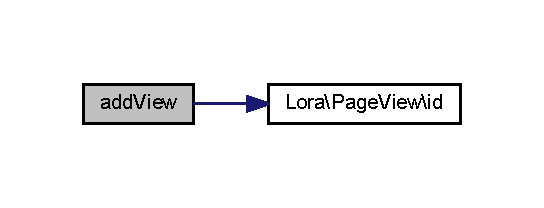
\includegraphics[width=261pt]{class_lora_1_1_page_a56b08acddd9971d439900b307e91f1f0_cgraph}
\end{center}
\end{figure}
\mbox{\label{class_lora_1_1_page_a3af53cb9d6437cde1e23d590488e683a}} 
\index{Lora\+::\+Page@{Lora\+::\+Page}!add\+Views@{add\+Views}}
\index{add\+Views@{add\+Views}!Lora\+::\+Page@{Lora\+::\+Page}}
\subsubsection{add\+Views()}
{\footnotesize\ttfamily add\+Views (\begin{DoxyParamCaption}\item[{array}]{\$views }\end{DoxyParamCaption})}

Adds multiple Page\+Views to this \doxyref{Page}{p.}{class_lora_1_1_page}. 
\begin{DoxyParams}{Parameters}
{\em \$views} & An array of \doxyref{Page\+View}{p.}{class_lora_1_1_page_view} objects. \\
\hline
\end{DoxyParams}

\begin{DoxyCode}
93                                             : \textcolor{keywordtype}{void} \{
94         \textcolor{keywordflow}{if} (\(\backslash\)DataLib::AreInstanceOf ($view, PageView::class)) \{
95             \textcolor{keywordflow}{foreach} ($views as $v) \{
96                 $this->view [$v->id ()] = $v;;
97             \}
98         \}
99     \}
\end{DoxyCode}
Here is the call graph for this function\+:\nopagebreak
\begin{figure}[H]
\begin{center}
\leavevmode
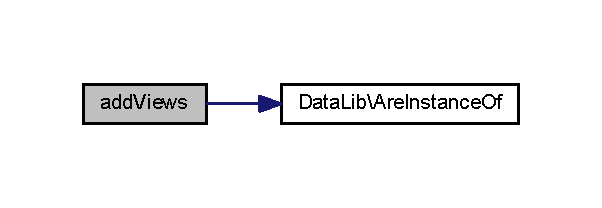
\includegraphics[width=289pt]{class_lora_1_1_page_a3af53cb9d6437cde1e23d590488e683a_cgraph}
\end{center}
\end{figure}
\mbox{\label{class_lora_1_1_page_a3b38056ae9a3c2cada8000895f46b9cb}} 
\index{Lora\+::\+Page@{Lora\+::\+Page}!configurable\+Fields@{configurable\+Fields}}
\index{configurable\+Fields@{configurable\+Fields}!Lora\+::\+Page@{Lora\+::\+Page}}
\subsubsection{configurable\+Fields()}
{\footnotesize\ttfamily configurable\+Fields (\begin{DoxyParamCaption}\item[{array}]{\$exclude = {\ttfamily []} }\end{DoxyParamCaption})\hspace{0.3cm}{\ttfamily [private]}}

Returns an array of property field names in this class which can be set using initialization files with \doxyref{Page\+::load\+View}{p.}{class_lora_1_1_page_a943f0df56a6f8dbc260ddb31925ce4f6}. 
\begin{DoxyParams}{Parameters}
{\em \$exclude} & An array containing field names which are to be excluded from the final collection. \\
\hline
\end{DoxyParams}
\begin{DoxyReturn}{Returns}
Returns an array of field names. It is possible for this array to be empty. 
\end{DoxyReturn}

\begin{DoxyCode}
406                                                               \{
407         \textcolor{keywordflow}{return} array\_filter (
408             array\_map (\textcolor{keyword}{function} ($field) \{ \textcolor{keywordflow}{return} $field->name; \}, (new \(\backslash\)ReflectionClass ($this))->
      getProperties ()),
409             \textcolor{keyword}{function} ($field) use ($exclude) \{
410                 \textcolor{keywordflow}{return} @$field [0] === \textcolor{charliteral}{'\_'} && !in\_array ($field, $exclude); \}
411         );
412     \}
\end{DoxyCode}
\mbox{\label{class_lora_1_1_page_a9b80bb36f89498eac4f43bf08461240d}} 
\index{Lora\+::\+Page@{Lora\+::\+Page}!content@{content}}
\index{content@{content}!Lora\+::\+Page@{Lora\+::\+Page}}
\subsubsection{content()}
{\footnotesize\ttfamily content (\begin{DoxyParamCaption}{ }\end{DoxyParamCaption})}

Returns the content file name of this page. Since all pages use the same base naming for files, there is no need to store it in any variable. \begin{DoxyReturn}{Returns}
Name of the content twig file. 
\end{DoxyReturn}

\begin{DoxyCode}
238                                : \textcolor{keywordtype}{string} \{
239         \textcolor{keywordflow}{return} \textcolor{stringliteral}{"content."}.Config::ext (\textcolor{stringliteral}{'twig'}, \textcolor{stringliteral}{'twig'});
240     \}
\end{DoxyCode}
\mbox{\label{class_lora_1_1_page_aaed74f7942d3fc56582e99324500e87b}} 
\index{Lora\+::\+Page@{Lora\+::\+Page}!debug@{debug}}
\index{debug@{debug}!Lora\+::\+Page@{Lora\+::\+Page}}
\subsubsection{debug()}
{\footnotesize\ttfamily debug (\begin{DoxyParamCaption}{ }\end{DoxyParamCaption})}

A wrapper function to allow twig to check if debugging is on. 
\begin{DoxyCode}
263                              : \textcolor{keywordtype}{bool} \{
264         return \(\backslash\)debug ();
265     \}
\end{DoxyCode}
\mbox{\label{class_lora_1_1_page_a9caaa1f5ea6177e55f13ebe7dec2bd60}} 
\index{Lora\+::\+Page@{Lora\+::\+Page}!finalize@{finalize}}
\index{finalize@{finalize}!Lora\+::\+Page@{Lora\+::\+Page}}
\subsubsection{finalize()}
{\footnotesize\ttfamily finalize (\begin{DoxyParamCaption}{ }\end{DoxyParamCaption})}

Finalizes page object loading and parses certain data structures into objects. \begin{DoxyRefDesc}{Todo}
\item[\textbf{ Todo}]Should be relocated. A possible place would be \doxyref{Page\+Manager}{p.}{class_lora_1_1_page_manager}. \end{DoxyRefDesc}

\begin{DoxyCode}
315                                 : \textcolor{keywordtype}{void} \{
316 \textcolor{preprocessor}{        # TODO: Write more complete page parser utility somewhere else.}
317         \textcolor{keywordflow}{if} (isset ($this->\_settings [\textcolor{stringliteral}{'side\_nav'}]) && is\_array ($this->\_settings [\textcolor{stringliteral}{'side\_nav'}])) \{
318             \textcolor{keywordflow}{foreach} ($this->\_settings [\textcolor{stringliteral}{'side\_nav'}] as &$entry) \{
319                 \textcolor{keywordflow}{foreach} ($entry [\textcolor{stringliteral}{'items'}] as $key => &$link) \{
320                     \textcolor{keywordflow}{if} (!is\_array ($link)) \{
321                         \textcolor{keywordflow}{continue};
322                     \}
323                     $params = isset ($link [\textcolor{stringliteral}{'params'}]) ? $link [\textcolor{stringliteral}{'params'}] : [];
324                     $target = isset ($link [\textcolor{stringliteral}{'target'}]) ? $link [\textcolor{stringliteral}{'target'}] : $this->
      name ();
325                     \textcolor{keywordflow}{if} (!isset ($link [\textcolor{stringliteral}{'text'}], $link [\textcolor{stringliteral}{'target'}]) || !is\_string ($link [\textcolor{stringliteral}{'text'}]) || !
      is\_string ($link [\textcolor{stringliteral}{'target'}]) || !is\_array ($params)) \{
326                         unset ($entry [\textcolor{stringliteral}{'items'}][$key]);
327                         \textcolor{keywordflow}{continue};
328                     \}
329                     $entry [\textcolor{stringliteral}{'items'}][$key] = new \(\backslash\)Html\(\backslash\)Link ($link [\textcolor{stringliteral}{'text'}], $link [\textcolor{stringliteral}{'target'}], $params);
330                 \}
331             \}
332         \}
333     \}
\end{DoxyCode}
\mbox{\label{class_lora_1_1_page_aebdf4663cb6825d8f47de13850be31bd}} 
\index{Lora\+::\+Page@{Lora\+::\+Page}!globals@{globals}}
\index{globals@{globals}!Lora\+::\+Page@{Lora\+::\+Page}}
\subsubsection{globals()}
{\footnotesize\ttfamily globals (\begin{DoxyParamCaption}{ }\end{DoxyParamCaption})}

Returns an array containing all global values in this \doxyref{Page}{p.}{class_lora_1_1_page}. \begin{DoxyReturn}{Returns}
An array of global javascript variables. 
\end{DoxyReturn}

\begin{DoxyCode}
181                                : array \{
182         \textcolor{comment}{/*}
183 \textcolor{comment}{        # Might be used later. Components require a way to define global values and there has to be a
       system for them to request such values.}
184 \textcolor{comment}{            foreach ($this->views as $view) \{}
185 \textcolor{comment}{                foreach ($view->components () as $comp) \{}
186 \textcolor{comment}{                    $this->\_globals = array\_merge ($this->\_globals, $comp->globals ());}
187 \textcolor{comment}{                \}}
188 \textcolor{comment}{            \}}
189 \textcolor{comment}{        */}
190         \textcolor{keywordflow}{return} $this->\_globals;
191     \}
\end{DoxyCode}
\mbox{\label{class_lora_1_1_page_a9b2dd808ffcd764782fb11b3ea583a8d}} 
\index{Lora\+::\+Page@{Lora\+::\+Page}!is\+Static@{is\+Static}}
\index{is\+Static@{is\+Static}!Lora\+::\+Page@{Lora\+::\+Page}}
\subsubsection{is\+Static()}
{\footnotesize\ttfamily is\+Static (\begin{DoxyParamCaption}{ }\end{DoxyParamCaption})}

\begin{DoxyReturn}{Returns}
Returns whether or not this \doxyref{Page}{p.}{class_lora_1_1_page} is considered static. 
\end{DoxyReturn}

\begin{DoxyCode}
77                                 : \textcolor{keywordtype}{bool} \{
78         \textcolor{keywordflow}{return} $this->static;
79     \}
\end{DoxyCode}
\mbox{\label{class_lora_1_1_page_a0e9447221830f8629717836bd933a164}} 
\index{Lora\+::\+Page@{Lora\+::\+Page}!layout@{layout}}
\index{layout@{layout}!Lora\+::\+Page@{Lora\+::\+Page}}
\subsubsection{layout()}
{\footnotesize\ttfamily layout (\begin{DoxyParamCaption}{ }\end{DoxyParamCaption})}

\begin{DoxyReturn}{Returns}
Returns name of the layout file for this \doxyref{Page}{p.}{class_lora_1_1_page}. 
\end{DoxyReturn}

\begin{DoxyCode}
229                               : \textcolor{keywordtype}{string} \{
230         \textcolor{keywordflow}{return} $this->\_layout = \Lib::checkExtension ($this->\_layout, 
      Config::ext (\textcolor{stringliteral}{'twig'}, \textcolor{stringliteral}{'twig'}));
231     \}
\end{DoxyCode}
Here is the call graph for this function\+:\nopagebreak
\begin{figure}[H]
\begin{center}
\leavevmode
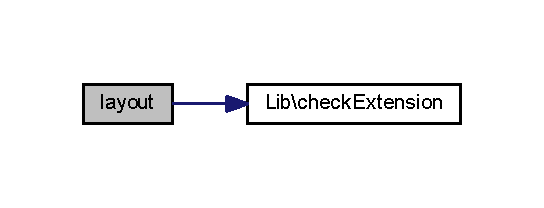
\includegraphics[width=261pt]{class_lora_1_1_page_a0e9447221830f8629717836bd933a164_cgraph}
\end{center}
\end{figure}
\mbox{\label{class_lora_1_1_page_af34d5049c9cc4ab108d65218754b7429}} 
\index{Lora\+::\+Page@{Lora\+::\+Page}!libraries@{libraries}}
\index{libraries@{libraries}!Lora\+::\+Page@{Lora\+::\+Page}}
\subsubsection{libraries()}
{\footnotesize\ttfamily libraries (\begin{DoxyParamCaption}{ }\end{DoxyParamCaption})}

Collects all javascript files from Page\+Views and their Page\+Components, inspects if they already exist within the collection and if not, adds them to it. Once all the scripts have been collected, they\textquotesingle{}re given file extensions as necessary. \begin{DoxyReturn}{Returns}
Returns all scripts this \doxyref{Page}{p.}{class_lora_1_1_page} has. 
\end{DoxyReturn}

\begin{DoxyCode}
153                                  : array \{
154         \textcolor{keywordflow}{foreach} ($this->views as $view) \{
155             \textcolor{keywordflow}{foreach} ($view->components () as $comp) \{
156                 $this->\_libraries = array\_unique (array\_merge ($this->\_libraries, $comp->libraries ()));
157             \}
158         \}
159         \textcolor{keywordflow}{foreach} ($this->\_libraries as &$lib) \{
160             $lib = \Lib::checkExtension ($lib, \textcolor{stringliteral}{'js'});
161         \} \textcolor{keywordflow}{return} $this->\_libraries;
162     \}
\end{DoxyCode}
Here is the call graph for this function\+:\nopagebreak
\begin{figure}[H]
\begin{center}
\leavevmode
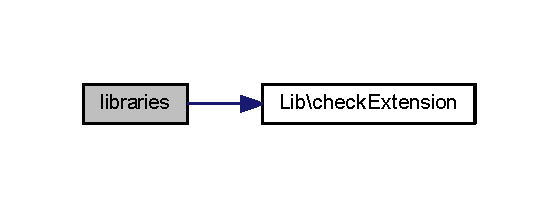
\includegraphics[width=268pt]{class_lora_1_1_page_af34d5049c9cc4ab108d65218754b7429_cgraph}
\end{center}
\end{figure}
\mbox{\label{class_lora_1_1_page_a943f0df56a6f8dbc260ddb31925ce4f6}} 
\index{Lora\+::\+Page@{Lora\+::\+Page}!load\+View@{load\+View}}
\index{load\+View@{load\+View}!Lora\+::\+Page@{Lora\+::\+Page}}
\subsubsection{load\+View()}
{\footnotesize\ttfamily load\+View (\begin{DoxyParamCaption}\item[{string}]{\$view }\end{DoxyParamCaption})}

\begin{DoxyRefDesc}{Todo}
\item[\textbf{ Todo}]Rename to load. Loads a \doxyref{Page}{p.}{class_lora_1_1_page} \end{DoxyRefDesc}

\begin{DoxyCode}
271                                             : \textcolor{keywordtype}{bool} \{
272         $this->view = $view;
273         $file = \textcolor{stringliteral}{"\{$this->\_path\}/\{$this->view\}/view."}.Config::ext (\textcolor{stringliteral}{'server'}, \textcolor{stringliteral}{'page'});
274         \textcolor{keywordflow}{if} (!file\_exists ($file) || empty ($config = $this->parseFile ($file)) || !$this->
      verifyConfig ($config)) \{
275             \textcolor{keywordflow}{return} \textcolor{keyword}{false};
276         \}
277         \textcolor{keywordflow}{foreach} ($this->configurableFields () as $member) \{
278             $property = substr ($member, 1);
279             \textcolor{keywordflow}{if} (isset ($config [$property]) && gettype ($config [$property]) === gettype ($this->$member)) 
      \{
280                 $this->$member = $config [$property];
281             \}
282         \}
283         \textcolor{keywordflow}{if} (is\_array ($config [\textcolor{stringliteral}{'views'}])) \{
284             $this->parseViews ($config [\textcolor{stringliteral}{'views'}]);
285         \}
286         \textcolor{keywordflow}{return} \textcolor{keyword}{true};
287     \}
\end{DoxyCode}
\mbox{\label{class_lora_1_1_page_ad9b0a8a1b47c6bfbacd35cb4570d408a}} 
\index{Lora\+::\+Page@{Lora\+::\+Page}!mark\+Static@{mark\+Static}}
\index{mark\+Static@{mark\+Static}!Lora\+::\+Page@{Lora\+::\+Page}}
\subsubsection{mark\+Static()}
{\footnotesize\ttfamily mark\+Static (\begin{DoxyParamCaption}{ }\end{DoxyParamCaption})}

Marks this \doxyref{Page}{p.}{class_lora_1_1_page} as static meaning that its contents will not change despite it being dynamically generated using a \doxyref{Content}{p.}{namespace_lora_1_1_content} -\/class. This enables caching the results and potentially skip the whole generation process. 
\begin{DoxyCode}
70                                   : \textcolor{keywordtype}{void} \{
71         $this->\textcolor{keyword}{static} = \textcolor{keyword}{true};
72     \}
\end{DoxyCode}
\mbox{\label{class_lora_1_1_page_a4b516aaa5fa38da4fed24ab6001627e2}} 
\index{Lora\+::\+Page@{Lora\+::\+Page}!name@{name}}
\index{name@{name}!Lora\+::\+Page@{Lora\+::\+Page}}
\subsubsection{name()}
{\footnotesize\ttfamily name (\begin{DoxyParamCaption}{ }\end{DoxyParamCaption})}

\begin{DoxyReturn}{Returns}
Returns view name for this \doxyref{Page}{p.}{class_lora_1_1_page}. 
\end{DoxyReturn}

\begin{DoxyCode}
36                             : \textcolor{keywordtype}{string} \{
37         \textcolor{keywordflow}{return} $this->view;
38     \}
\end{DoxyCode}
Here is the caller graph for this function\+:\nopagebreak
\begin{figure}[H]
\begin{center}
\leavevmode
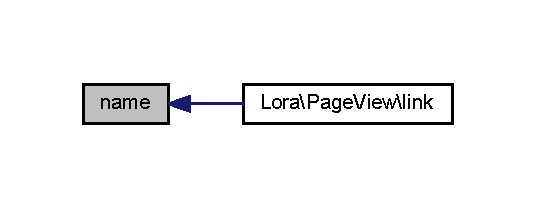
\includegraphics[width=257pt]{class_lora_1_1_page_a4b516aaa5fa38da4fed24ab6001627e2_icgraph}
\end{center}
\end{figure}
\mbox{\label{class_lora_1_1_page_a63ba1656485acf76a0d23e8f64fdfa1d}} 
\index{Lora\+::\+Page@{Lora\+::\+Page}!parse\+File@{parse\+File}}
\index{parse\+File@{parse\+File}!Lora\+::\+Page@{Lora\+::\+Page}}
\subsubsection{parse\+File()}
{\footnotesize\ttfamily parse\+File (\begin{DoxyParamCaption}\item[{string}]{\$file }\end{DoxyParamCaption})\hspace{0.3cm}{\ttfamily [private]}}

Reads in a value file comtaining property values for this object. 
\begin{DoxyParams}{Parameters}
{\em \$file} & Full path of the file containing property values. Can be an I\+NI or J\+S\+ON file. \\
\hline
\end{DoxyParams}
\begin{DoxyReturn}{Returns}
Returns an array of property values on success or an empty array on failure. 
\end{DoxyReturn}

\begin{DoxyCode}
386                                               : array \{
387         \textcolor{keywordflow}{if} (empty ($config = @parse\_ini\_file ($file, \textcolor{keyword}{true}, INI\_SCANNER\_TYPED)) && empty ($config = @
      json\_decode (file\_get\_contents ($file), \textcolor{keyword}{true}))) \{
388             \textcolor{keywordflow}{return} [];
389         \}
390         \textcolor{keywordflow}{return} $config;
391     \}
\end{DoxyCode}
\mbox{\label{class_lora_1_1_page_a49b28f2ca7604e14af0d5829b4e8cc4a}} 
\index{Lora\+::\+Page@{Lora\+::\+Page}!parse\+Views@{parse\+Views}}
\index{parse\+Views@{parse\+Views}!Lora\+::\+Page@{Lora\+::\+Page}}
\subsubsection{parse\+Views()}
{\footnotesize\ttfamily parse\+Views (\begin{DoxyParamCaption}\item[{array}]{\$views }\end{DoxyParamCaption})\hspace{0.3cm}{\ttfamily [private]}}

Parses \doxyref{Page\+View}{p.}{class_lora_1_1_page_view} data and creates new instances of them based on the page configuration file. Succesfully created Page\+Views are added to this \doxyref{Page}{p.}{class_lora_1_1_page}. \begin{DoxyRefDesc}{Todo}
\item[\textbf{ Todo}]Needs cleaning \end{DoxyRefDesc}

\begin{DoxyParams}{Parameters}
{\em \$views} & An array containing view configurations from which new Page\+Views will be created \\
\hline
\end{DoxyParams}

\begin{DoxyCode}
341                                                \{
342         \textcolor{keywordflow}{if} (!isset ($views [\textcolor{stringliteral}{'views'}]) || !is\_array ($views [\textcolor{stringliteral}{'views'}])) \{
343             \textcolor{keywordflow}{return};
344         \}
345         \textcolor{keywordflow}{foreach} ($views [\textcolor{stringliteral}{'views'}] as $view) \{
346             \textcolor{keywordflow}{if} (!is\_array ($view) || !isset ($view [\textcolor{stringliteral}{'name'}])) \{
347                 \textcolor{keywordflow}{continue};
348             \}
349             $pv = \textcolor{keyword}{new} PageView ();
350             $pv->load ($view);
351             \textcolor{keywordflow}{if} (isset ($view [\textcolor{stringliteral}{'default'}])) \{
352                 $pv->show ($view [\textcolor{stringliteral}{'default'}] === \textcolor{keyword}{true});
353             \}
354             $this->views [$pv->id ()] = $pv;
355         \}
356         $this->\_settings [\textcolor{stringliteral}{'side\_nav'}] = [];
357         \textcolor{keywordflow}{if} (isset ($views [\textcolor{stringliteral}{'navigation'}]) && is\_array ($views [\textcolor{stringliteral}{'navigation'}])) \{
358             \textcolor{keywordflow}{foreach} ($views [\textcolor{stringliteral}{'navigation'}] as $entry) \{
359                 \textcolor{keywordflow}{if} (!is\_array ($entry)) \{
360                     \textcolor{keywordflow}{continue};
361                 \}
362                 $heading = isset ($entry [\textcolor{stringliteral}{'heading'}]) && is\_string ($entry [\textcolor{stringliteral}{'heading'}]) ? $entry [\textcolor{stringliteral}{'heading'}
      ] : \textcolor{stringliteral}{''};
363                 $items = isset ($entry [\textcolor{stringliteral}{'items'}]) && is\_array ($entry [\textcolor{stringliteral}{'items'}]) ? $entry [\textcolor{stringliteral}{'items'}] : [];
364                 $entry = [ \textcolor{stringliteral}{'heading'} => $heading, \textcolor{stringliteral}{'items'} => [] ];
365                 \textcolor{keywordflow}{foreach} ($items as $link) \{
366                     $view = isset ($link [\textcolor{stringliteral}{'view'}]) && is\_string ($link [\textcolor{stringliteral}{'view'}]) ? $link [\textcolor{stringliteral}{'view'}] : \textcolor{stringliteral}{''};
367                     $text = isset ($link [\textcolor{stringliteral}{'text'}]) && is\_string ($link [\textcolor{stringliteral}{'text'}]) ? $link [\textcolor{stringliteral}{'text'}] : \textcolor{stringliteral}{''};
368                     \textcolor{keywordflow}{if} (!empty ($temp = $this->views [$link [\textcolor{stringliteral}{'view'}]])) \{
369                         $entry [\textcolor{stringliteral}{'items'}][] = $temp->link ($this, $text);
370                     \} \textcolor{keywordflow}{else} \{
371                         $target = isset ($link [\textcolor{stringliteral}{'target'}]) && is\_string ($link [\textcolor{stringliteral}{'target'}]) ? $link [\textcolor{stringliteral}{'target
      '}] : \textcolor{stringliteral}{''};
372                         $params = isset ($link [\textcolor{stringliteral}{'params'}]) && is\_array ($link [\textcolor{stringliteral}{'params'}]) ? $link [\textcolor{stringliteral}{'params'}
      ] : [];
373                         $entry [\textcolor{stringliteral}{'items'}][] = [ \textcolor{stringliteral}{'text'} => $text, \textcolor{stringliteral}{'params'} => $params, \textcolor{stringliteral}{'target'} => $target ];
374                     \}
375                 \}
376                 $this->\_settings [\textcolor{stringliteral}{'side\_nav'}][] = $entry;
377             \}
378         \}
379     \}
\end{DoxyCode}
\mbox{\label{class_lora_1_1_page_a3b05eec13add53df44e232273d718ae4}} 
\index{Lora\+::\+Page@{Lora\+::\+Page}!path@{path}}
\index{path@{path}!Lora\+::\+Page@{Lora\+::\+Page}}
\subsubsection{path()}
{\footnotesize\ttfamily path (\begin{DoxyParamCaption}{ }\end{DoxyParamCaption})}

\begin{DoxyReturn}{Returns}
Returns path to this \doxyref{Page}{p.}{class_lora_1_1_page}\textquotesingle{}s view folder. 
\end{DoxyReturn}

\begin{DoxyCode}
215                             : \textcolor{keywordtype}{string} \{
216         \textcolor{keywordflow}{return} \textcolor{stringliteral}{"\{$this->\_path\}/\{$this->view\}"};
217     \}
\end{DoxyCode}
\mbox{\label{class_lora_1_1_page_a3dc593f496b7dbf2e5e3c406cb5fd106}} 
\index{Lora\+::\+Page@{Lora\+::\+Page}!scripts@{scripts}}
\index{scripts@{scripts}!Lora\+::\+Page@{Lora\+::\+Page}}
\subsubsection{scripts()}
{\footnotesize\ttfamily scripts (\begin{DoxyParamCaption}{ }\end{DoxyParamCaption})}

Collects all javascript file names from Page\+Views and their Page\+Components, inspects if they already exist within the collection and if not, adds them to it. Once all the scripts have been collected, they\textquotesingle{}re given file extensions as necessary. \begin{DoxyReturn}{Returns}
Returns all scripts this \doxyref{Page}{p.}{class_lora_1_1_page} has. 
\end{DoxyReturn}

\begin{DoxyCode}
125                                : array \{
126         \textcolor{keywordflow}{foreach} ($this->views as $view) \{
127             \textcolor{keywordflow}{foreach} ($view->components () as $comp) \{
128                 $this->\_scripts = array\_unique (array\_merge ($this->\_scripts, $comp->scripts ()));
129             \}
130         \}
131         \textcolor{keywordflow}{foreach} ($this->\_scripts as &$script) \{
132             $script = \Lib::checkExtension ($script, \textcolor{stringliteral}{'js'});
133         \} \textcolor{keywordflow}{return} $this->\_scripts;
134     \}
\end{DoxyCode}
Here is the call graph for this function\+:\nopagebreak
\begin{figure}[H]
\begin{center}
\leavevmode
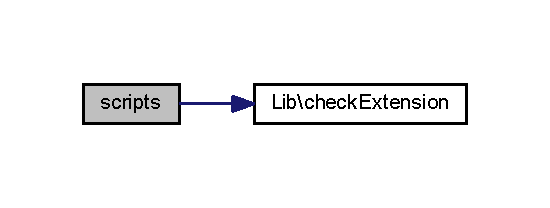
\includegraphics[width=264pt]{class_lora_1_1_page_a3dc593f496b7dbf2e5e3c406cb5fd106_cgraph}
\end{center}
\end{figure}
\mbox{\label{class_lora_1_1_page_a1d32f1ec82bc539460db5c0666b18a76}} 
\index{Lora\+::\+Page@{Lora\+::\+Page}!set\+Setting@{set\+Setting}}
\index{set\+Setting@{set\+Setting}!Lora\+::\+Page@{Lora\+::\+Page}}
\subsubsection{set\+Setting()}
{\footnotesize\ttfamily set\+Setting (\begin{DoxyParamCaption}\item[{}]{\$detail,  }\item[{string}]{\$key }\end{DoxyParamCaption})}

Allows settings a value to this \doxyref{Page}{p.}{class_lora_1_1_page} under certain key. An outdated method but still required in some places. 
\begin{DoxyParams}{Parameters}
{\em \$detail} & A value to be stored in this \doxyref{Page}{p.}{class_lora_1_1_page}. \\
\hline
{\em \$key} & A key under which the value is stored. \\
\hline
\end{DoxyParams}

\begin{DoxyCode}
199                                                       : \textcolor{keywordtype}{void} \{
200         $this->\_settings [$key] = $detail;
201     \}
\end{DoxyCode}
\mbox{\label{class_lora_1_1_page_ad7354383714c6ae99d6ee1bfb95ab49f}} 
\index{Lora\+::\+Page@{Lora\+::\+Page}!settings@{settings}}
\index{settings@{settings}!Lora\+::\+Page@{Lora\+::\+Page}}
\subsubsection{settings()}
{\footnotesize\ttfamily settings (\begin{DoxyParamCaption}{ }\end{DoxyParamCaption})}

Quite out dated function but some functionality still relies on it so it shall remain here for now. Overall better solutions are required for multiple sections of the \doxyref{Page}{p.}{class_lora_1_1_page} management system. \begin{DoxyReturn}{Returns}
Returns all settings this \doxyref{Page}{p.}{class_lora_1_1_page} has. 
\end{DoxyReturn}

\begin{DoxyCode}
208                                 : array \{
209         \textcolor{keywordflow}{return} $this->\_settings;
210     \}
\end{DoxyCode}
\mbox{\label{class_lora_1_1_page_a4bf70b1d635601a513ff8f2c31a9111a}} 
\index{Lora\+::\+Page@{Lora\+::\+Page}!show@{show}}
\index{show@{show}!Lora\+::\+Page@{Lora\+::\+Page}}
\subsubsection{show()}
{\footnotesize\ttfamily show (\begin{DoxyParamCaption}\item[{string}]{\$view\+Name,  }\item[{bool}]{\$show }\end{DoxyParamCaption})}

Changes visibility of a subview (\doxyref{Page\+View}{p.}{class_lora_1_1_page_view}). 
\begin{DoxyParams}{Parameters}
{\em \$view} & Name of the subview to apply the visibility status to. \\
\hline
{\em \$show} & A boolean value to determine the visibility of the subview. \\
\hline
\end{DoxyParams}

\begin{DoxyCode}
45                                                         : \textcolor{keywordtype}{void} \{
46         \textcolor{keywordflow}{if} (isset ($this->views [$viewName])) \{
47             $this->views [$viewName]->show ($show);
48         \}
49     \}
\end{DoxyCode}
\mbox{\label{class_lora_1_1_page_a3aa8e55512ba551535b423e88ec4c9b1}} 
\index{Lora\+::\+Page@{Lora\+::\+Page}!show\+Single@{show\+Single}}
\index{show\+Single@{show\+Single}!Lora\+::\+Page@{Lora\+::\+Page}}
\subsubsection{show\+Single()}
{\footnotesize\ttfamily show\+Single (\begin{DoxyParamCaption}\item[{string}]{\$view\+Name }\end{DoxyParamCaption})}

Hides all but one subview if a subview with a given name exist. As a side effect, if a view with the given name does not exist, all the views are hidden. 
\begin{DoxyParams}{Parameters}
{\em \$view\+Name} & Name of the view that becomes visible. \\
\hline
\end{DoxyParams}

\begin{DoxyCode}
57                                                   : \textcolor{keywordtype}{void} \{
58         \textcolor{keywordflow}{foreach} ($this->views as $v) \{
59             $v->show (\textcolor{keyword}{false});
60         \}
61         $this->show ($viewName, \textcolor{keyword}{true});
62     \}
\end{DoxyCode}
\mbox{\label{class_lora_1_1_page_aac68ba2faa04ea9430b52d4de572d085}} 
\index{Lora\+::\+Page@{Lora\+::\+Page}!side\+Panel@{side\+Panel}}
\index{side\+Panel@{side\+Panel}!Lora\+::\+Page@{Lora\+::\+Page}}
\subsubsection{side\+Panel()}
{\footnotesize\ttfamily side\+Panel (\begin{DoxyParamCaption}{ }\end{DoxyParamCaption})}

This is a bit hacky solution and a better one should be created which supports all panels and not just a single one. \begin{DoxyReturn}{Returns}
Returns left side panel related data, mostly hyperlink objects. 
\end{DoxyReturn}

\begin{DoxyCode}
294                                  \{
295         \textcolor{keywordflow}{return} $this->\_settings [\textcolor{stringliteral}{'side\_nav'}];
296     \}
\end{DoxyCode}
\mbox{\label{class_lora_1_1_page_a53d31780f290c90071a213e9f786abb3}} 
\index{Lora\+::\+Page@{Lora\+::\+Page}!styles@{styles}}
\index{styles@{styles}!Lora\+::\+Page@{Lora\+::\+Page}}
\subsubsection{styles()}
{\footnotesize\ttfamily styles (\begin{DoxyParamCaption}{ }\end{DoxyParamCaption})}

Collects all css files from Page\+Views and their Page\+Components, inspects if they already exist within the collection and if not, adds them to it. Once all the css files have been collected, they\textquotesingle{}re given file extensions as necessary. \begin{DoxyReturn}{Returns}
Returns all css files this \doxyref{Page}{p.}{class_lora_1_1_page} has. 
\end{DoxyReturn}

\begin{DoxyCode}
249                               : array \{
250         \textcolor{keywordflow}{foreach} ($this->views as $view) \{
251             \textcolor{keywordflow}{foreach} ($view->components () as $comp) \{
252                 $this->\_styles = array\_unique (array\_merge ($this->\_styles, $comp->styles ()));
253             \}
254         \}
255         \textcolor{keywordflow}{foreach} ($this->\_styles as &$style) \{
256             $style = \Lib::checkExtension ($style, \textcolor{stringliteral}{'css'});
257         \} \textcolor{keywordflow}{return} $this->\_styles;
258     \}
\end{DoxyCode}
Here is the call graph for this function\+:\nopagebreak
\begin{figure}[H]
\begin{center}
\leavevmode
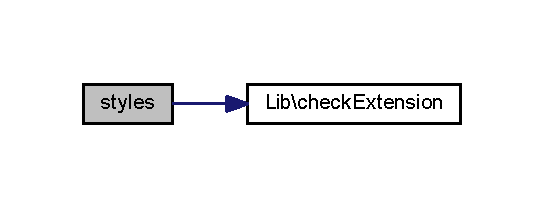
\includegraphics[width=261pt]{class_lora_1_1_page_a53d31780f290c90071a213e9f786abb3_cgraph}
\end{center}
\end{figure}
\mbox{\label{class_lora_1_1_page_a420c4b91157962374150f731a2ac57dc}} 
\index{Lora\+::\+Page@{Lora\+::\+Page}!sub\+Views@{sub\+Views}}
\index{sub\+Views@{sub\+Views}!Lora\+::\+Page@{Lora\+::\+Page}}
\subsubsection{sub\+Views()}
{\footnotesize\ttfamily sub\+Views (\begin{DoxyParamCaption}{ }\end{DoxyParamCaption})}

\begin{DoxyReturn}{Returns}
Returns all \doxyref{Page\+View}{p.}{class_lora_1_1_page_view} objects this \doxyref{Page}{p.}{class_lora_1_1_page} has. 
\end{DoxyReturn}

\begin{DoxyCode}
104                                 : array \{
105         \textcolor{keywordflow}{return} $this->views;
106     \}
\end{DoxyCode}
\mbox{\label{class_lora_1_1_page_a0b54c9d3801b331b75487ef78d98c06b}} 
\index{Lora\+::\+Page@{Lora\+::\+Page}!template@{template}}
\index{template@{template}!Lora\+::\+Page@{Lora\+::\+Page}}
\subsubsection{template()}
{\footnotesize\ttfamily template (\begin{DoxyParamCaption}{ }\end{DoxyParamCaption})}

\begin{DoxyReturn}{Returns}
Returns name of the template file for this \doxyref{Page}{p.}{class_lora_1_1_page}. 
\end{DoxyReturn}

\begin{DoxyCode}
222                                 : \textcolor{keywordtype}{string} \{
223         \textcolor{keywordflow}{return} $this->\_template = \Lib::checkExtension ($this->\_template, 
      Config::ext (\textcolor{stringliteral}{'twig'}, \textcolor{stringliteral}{'twig'}));
224     \}
\end{DoxyCode}
Here is the call graph for this function\+:\nopagebreak
\begin{figure}[H]
\begin{center}
\leavevmode
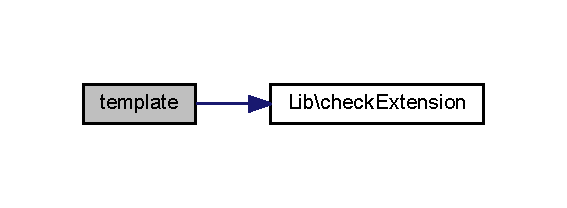
\includegraphics[width=272pt]{class_lora_1_1_page_a0b54c9d3801b331b75487ef78d98c06b_cgraph}
\end{center}
\end{figure}
\mbox{\label{class_lora_1_1_page_a163d90b496da60a48073aa5d127922ed}} 
\index{Lora\+::\+Page@{Lora\+::\+Page}!verify\+Config@{verify\+Config}}
\index{verify\+Config@{verify\+Config}!Lora\+::\+Page@{Lora\+::\+Page}}
\subsubsection{verify\+Config()}
{\footnotesize\ttfamily verify\+Config (\begin{DoxyParamCaption}\item[{array}]{\$config }\end{DoxyParamCaption})\hspace{0.3cm}{\ttfamily [private]}}

Verifies that a loaded page file is sane and can be used. \begin{DoxyReturn}{Returns}
Returns true if page config is valid and false if not. 
\end{DoxyReturn}

\begin{DoxyCode}
397                                                   \{
398         \textcolor{keywordflow}{return} isset ($config [\textcolor{stringliteral}{'views'}]);
399     \}
\end{DoxyCode}


The documentation for this class was generated from the following file\+:\begin{DoxyCompactItemize}
\item 
servers/webserver/server/page.\+php\end{DoxyCompactItemize}

\section{Page\+Component Class Reference}
\label{class_lora_1_1_page_component}\index{Page\+Component@{Page\+Component}}
\subsection*{Public Member Functions}
\begin{DoxyCompactItemize}
\item 
\textbf{ id} ()
\item 
\mbox{\label{class_lora_1_1_page_component_a30bd23795f307541c79fd2332dcf4af1}} 
{\bfseries set\+Template} (string \$\textbf{ template})
\item 
\textbf{ template} ()
\item 
\textbf{ add\+Script} (string \$script)
\item 
\textbf{ scripts} ()
\item 
\textbf{ add\+Library} (string \$lib)
\item 
\textbf{ libraries} ()
\item 
\textbf{ styles} ()
\item 
\textbf{ classes} (bool \$string=false)
\end{DoxyCompactItemize}
\subsection*{Static Public Member Functions}
\begin{DoxyCompactItemize}
\item 
static \textbf{ Create} (string \$component)
\end{DoxyCompactItemize}
\subsection*{Data Fields}
\begin{DoxyCompactItemize}
\item 
\mbox{\label{class_lora_1_1_page_component_a353afce17912a98c6a9ead92e679570d}} 
{\bfseries \$\+\_\+template} = \textquotesingle{}\textquotesingle{}
\item 
\mbox{\label{class_lora_1_1_page_component_a8ad159a11a3bfceca008de351d6fbebc}} 
{\bfseries \$\+\_\+libraries} = [$\,$]
\item 
\mbox{\label{class_lora_1_1_page_component_a714e6e780b17b3b8e7db069f2a96a119}} 
{\bfseries \$\+\_\+scripts} = [$\,$]
\item 
\mbox{\label{class_lora_1_1_page_component_a9c54ba83a52cee3c5a4b47dea3412c53}} 
{\bfseries \$\+\_\+styles} = [$\,$]
\item 
\mbox{\label{class_lora_1_1_page_component_a429c9bf2a1a7123e7d350631751eff67}} 
{\bfseries \$\+\_\+classes} = [$\,$]
\end{DoxyCompactItemize}
\subsection*{Private Member Functions}
\begin{DoxyCompactItemize}
\item 
\textbf{ configurable\+Fields} (array \$exclude=[$\,$])
\item 
\textbf{ parse\+File} (string \$file)
\item 
\textbf{ inspect\+Config} (array \$config)
\item 
\textbf{ populate} (array \$values)
\end{DoxyCompactItemize}
\subsection*{Private Attributes}
\begin{DoxyCompactItemize}
\item 
\mbox{\label{class_lora_1_1_page_component_a64da16c4a1c7b2dc6784f6ef26341ed7}} 
{\bfseries \$\+\_\+id} = \textquotesingle{}\textquotesingle{}
\end{DoxyCompactItemize}


\subsection{Detailed Description}
A class to represent Page\+Components. A component is essentially a collection of few configuration and dependency files. \doxyref{Configuration}{p.}{class_lora_1_1_configuration} files at the time of writing use component as their extension and their preferred file format is J\+S\+ON. Components also have a twig file of the same name as the component file. Twig files contain the H\+T\+ML a component requires to display it contents. \doxyref{Configuration}{p.}{class_lora_1_1_configuration} file contains all the dependencies and some other properties for the H\+T\+ML. This class might later be moved to  -\/namespace. 

\subsection{Member Function Documentation}
\mbox{\label{class_lora_1_1_page_component_acd0b83bc65713449f479130693bf4dbc}} 
\index{Lora\+::\+Page\+Component@{Lora\+::\+Page\+Component}!add\+Library@{add\+Library}}
\index{add\+Library@{add\+Library}!Lora\+::\+Page\+Component@{Lora\+::\+Page\+Component}}
\subsubsection{add\+Library()}
{\footnotesize\ttfamily add\+Library (\begin{DoxyParamCaption}\item[{string}]{\$lib }\end{DoxyParamCaption})}

Adds a new library to this \doxyref{Page\+Component}{p.}{class_lora_1_1_page_component}. These libraries are located in public/assets/ext. 
\begin{DoxyParams}{Parameters}
{\em \$lid} & Name of the library to be added. \\
\hline
\end{DoxyParams}

\begin{DoxyCode}
102                                              : \textcolor{keywordtype}{void} \{
103         \textcolor{keywordflow}{if} (!in\_array ($lib, $this->\_libraries)) \{
104             $this->\_libraries [] = $lib;
105         \}
106     \}
\end{DoxyCode}
\mbox{\label{class_lora_1_1_page_component_aa1c1a80393db2b30ad535b13de050778}} 
\index{Lora\+::\+Page\+Component@{Lora\+::\+Page\+Component}!add\+Script@{add\+Script}}
\index{add\+Script@{add\+Script}!Lora\+::\+Page\+Component@{Lora\+::\+Page\+Component}}
\subsubsection{add\+Script()}
{\footnotesize\ttfamily add\+Script (\begin{DoxyParamCaption}\item[{string}]{\$script }\end{DoxyParamCaption})}

Adds a new script to this \doxyref{Page\+Component}{p.}{class_lora_1_1_page_component}. These scripts are located in public/assets/scripts. 
\begin{DoxyParams}{Parameters}
{\em \$script} & Name of the script to be added. \\
\hline
\end{DoxyParams}

\begin{DoxyCode}
81                                                : \textcolor{keywordtype}{void} \{
82         \textcolor{keywordflow}{if} (!in\_array ($script, $this->\_scripts)) \{
83             $this->\_scripts [] = $script;
84         \}
85     \}
\end{DoxyCode}
\mbox{\label{class_lora_1_1_page_component_af6ac36c4e10b38c61aa0b45fa736bfc4}} 
\index{Lora\+::\+Page\+Component@{Lora\+::\+Page\+Component}!classes@{classes}}
\index{classes@{classes}!Lora\+::\+Page\+Component@{Lora\+::\+Page\+Component}}
\subsubsection{classes()}
{\footnotesize\ttfamily classes (\begin{DoxyParamCaption}\item[{bool}]{\$string = {\ttfamily false} }\end{DoxyParamCaption})}

If \$string is provided, it is added to the classes assigned to this \doxyref{Page\+Component}{p.}{class_lora_1_1_page_component}. If \$string is not provided, a string consisting of all class names separated by space will be returned. \begin{DoxyReturn}{Returns}
Returns a string of css classes. 
\end{DoxyReturn}

\begin{DoxyCode}
135                                                    \{
136         \textcolor{keywordflow}{if} ($string) \{
137             $classes = \textcolor{stringliteral}{''};
138             \textcolor{keywordflow}{foreach} ($this->\_classes as $c) \{
139                 $classes .= \textcolor{stringliteral}{"$c "};
140             \} \textcolor{keywordflow}{return} $classes;
141         \} \textcolor{keywordflow}{return} $this->\_classes;
142     \}
\end{DoxyCode}
\mbox{\label{class_lora_1_1_page_component_a3b38056ae9a3c2cada8000895f46b9cb}} 
\index{Lora\+::\+Page\+Component@{Lora\+::\+Page\+Component}!configurable\+Fields@{configurable\+Fields}}
\index{configurable\+Fields@{configurable\+Fields}!Lora\+::\+Page\+Component@{Lora\+::\+Page\+Component}}
\subsubsection{configurable\+Fields()}
{\footnotesize\ttfamily configurable\+Fields (\begin{DoxyParamCaption}\item[{array}]{\$exclude = {\ttfamily []} }\end{DoxyParamCaption})\hspace{0.3cm}{\ttfamily [private]}}

Returns an array of property field names in this class which can be set using initialization files with \doxyref{Page\+Component\+::populate}{p.}{class_lora_1_1_page_component_a8a5a7e2a8a27e02e0e68243d88ee339c}. 
\begin{DoxyParams}{Parameters}
{\em \$exclude} & An array containing field names which are to be excluded from the final collection. \\
\hline
\end{DoxyParams}
\begin{DoxyReturn}{Returns}
Returns an array of field names. It is possible for this array to be empty. 
\end{DoxyReturn}

\begin{DoxyCode}
149                                                               \{
150         \textcolor{keywordflow}{return} array\_filter (
151             array\_map (\textcolor{keyword}{function} ($field) \{ \textcolor{keywordflow}{return} $field->name; \}, (new \(\backslash\)ReflectionClass ($this))->
      getProperties ()),
152             \textcolor{keyword}{function} ($field) use ($exclude) \{
153                 \textcolor{keywordflow}{return} @$field [0] === \textcolor{charliteral}{'\_'} && !in\_array ($field, $exclude); \}
154         );
155     \}
\end{DoxyCode}
\mbox{\label{class_lora_1_1_page_component_ab6c03d0ec66cb31bfc74a784387cef33}} 
\index{Lora\+::\+Page\+Component@{Lora\+::\+Page\+Component}!Create@{Create}}
\index{Create@{Create}!Lora\+::\+Page\+Component@{Lora\+::\+Page\+Component}}
\subsubsection{Create()}
{\footnotesize\ttfamily static Create (\begin{DoxyParamCaption}\item[{string}]{\$component }\end{DoxyParamCaption})\hspace{0.3cm}{\ttfamily [static]}}

Creates a new \doxyref{Page\+Component}{p.}{class_lora_1_1_page_component} instance from a component name. Also populates all properties using component file of a same name. 
\begin{DoxyParams}{Parameters}
{\em \$component} & Name of the component. \\
\hline
\end{DoxyParams}
\begin{DoxyReturn}{Returns}
Returns a \doxyref{Page\+Component}{p.}{class_lora_1_1_page_component} instance. This component may be imcomplete if its component or template files are not working. 
\end{DoxyReturn}

\begin{DoxyCode}
36                                                       \{
37         $temp               = \textcolor{keyword}{new} PageComponent ();
38         $twig               = \Lib::checkExtension ($component, Config::ext (\textcolor{stringliteral}{'twig'}, \textcolor{stringliteral}{'twig'}));
39         $definition         = \Lib::checkExtension ($component, Config::ext (\textcolor{stringliteral}{'server'}, \textcolor{stringliteral}{'component'}));
40         $folder             = Config::path (\textcolor{stringliteral}{'server'}, \textcolor{stringliteral}{'components'});
41         $file               = \textcolor{stringliteral}{"$folder/$definition"};
42         \textcolor{keywordflow}{if} (file\_exists ($file)) \{
43             \textcolor{keywordflow}{if} (empty ($config = $temp->parseFile ($file)) || !$temp->inspectConfig ($config)) \{
44                 \textcolor{keywordflow}{return} null;
45             \}
46             $temp->\_id = $config [\textcolor{stringliteral}{'id'}];
47             $temp->\_template = $config [\textcolor{stringliteral}{'template'}];
48             $temp->populate ($config [\textcolor{stringliteral}{'dependencies'}]);
49             $temp->populate ($config [\textcolor{stringliteral}{'appearance'}]);
50         \} \textcolor{keywordflow}{else} \textcolor{keywordflow}{if} (file\_exists ($file = \textcolor{stringliteral}{"$folder/$twig"})) \{
51             $this->\_template = $file;
52             $this->\_id = pathinfo ($component, PATHINFO\_FILENAME);
53         \} \textcolor{keywordflow}{else} \{
54             \textcolor{keywordflow}{return} null;
55         \}
56         \textcolor{keywordflow}{return} $temp;
57     \}
\end{DoxyCode}
Here is the call graph for this function\+:\nopagebreak
\begin{figure}[H]
\begin{center}
\leavevmode
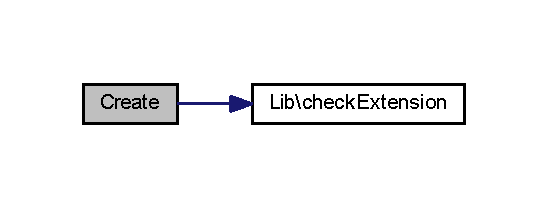
\includegraphics[width=263pt]{class_lora_1_1_page_component_ab6c03d0ec66cb31bfc74a784387cef33_cgraph}
\end{center}
\end{figure}
\mbox{\label{class_lora_1_1_page_component_a087060b582403885d08e89ad894ecc5d}} 
\index{Lora\+::\+Page\+Component@{Lora\+::\+Page\+Component}!id@{id}}
\index{id@{id}!Lora\+::\+Page\+Component@{Lora\+::\+Page\+Component}}
\subsubsection{id()}
{\footnotesize\ttfamily id (\begin{DoxyParamCaption}{ }\end{DoxyParamCaption})}

\begin{DoxyReturn}{Returns}
Returns id of this \doxyref{Page\+Component}{p.}{class_lora_1_1_page_component}. 
\end{DoxyReturn}

\begin{DoxyCode}
62                           \{
63         \textcolor{keywordflow}{return} $this->\_id;
64     \}
\end{DoxyCode}
\mbox{\label{class_lora_1_1_page_component_a836e6e03df9ed37584042af4708928d6}} 
\index{Lora\+::\+Page\+Component@{Lora\+::\+Page\+Component}!inspect\+Config@{inspect\+Config}}
\index{inspect\+Config@{inspect\+Config}!Lora\+::\+Page\+Component@{Lora\+::\+Page\+Component}}
\subsubsection{inspect\+Config()}
{\footnotesize\ttfamily inspect\+Config (\begin{DoxyParamCaption}\item[{array}]{\$config }\end{DoxyParamCaption})\hspace{0.3cm}{\ttfamily [private]}}

Verifies that a loaded component file is sane and can be used. \begin{DoxyReturn}{Returns}
Returns true if component config is valid and false if not. 
\end{DoxyReturn}

\begin{DoxyCode}
173                                                    : \textcolor{keywordtype}{bool} \{
174 \textcolor{preprocessor}{        # TODO?: Type checks}
175         \textcolor{keywordflow}{return} isset ($config [\textcolor{stringliteral}{'id'}], $config [\textcolor{stringliteral}{'template'}], $config [\textcolor{stringliteral}{'dependencies'}], $config [\textcolor{stringliteral}{'appearance'}
      ]);
176     \}
\end{DoxyCode}
\mbox{\label{class_lora_1_1_page_component_af34d5049c9cc4ab108d65218754b7429}} 
\index{Lora\+::\+Page\+Component@{Lora\+::\+Page\+Component}!libraries@{libraries}}
\index{libraries@{libraries}!Lora\+::\+Page\+Component@{Lora\+::\+Page\+Component}}
\subsubsection{libraries()}
{\footnotesize\ttfamily libraries (\begin{DoxyParamCaption}{ }\end{DoxyParamCaption})}

Returns an array containing all libraries assigned to this component. Goes through all of them and adds file extension to them if needed. \begin{DoxyReturn}{Returns}
Returns an array of file names. 
\end{DoxyReturn}

\begin{DoxyCode}
113                                  : array \{
114         \textcolor{keywordflow}{foreach} ($this->\_libraries as &$lib) \{
115             $lib = \Lib::checkExtension ($lib, \textcolor{stringliteral}{'js'});
116         \} \textcolor{keywordflow}{return} $this->\_libraries;
117     \}
\end{DoxyCode}
Here is the call graph for this function\+:\nopagebreak
\begin{figure}[H]
\begin{center}
\leavevmode
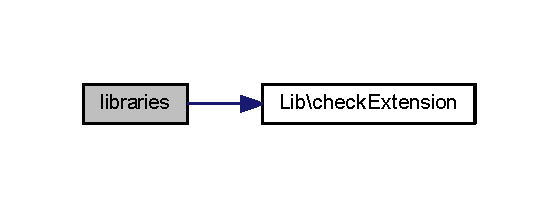
\includegraphics[width=268pt]{class_lora_1_1_page_component_af34d5049c9cc4ab108d65218754b7429_cgraph}
\end{center}
\end{figure}
\mbox{\label{class_lora_1_1_page_component_a63ba1656485acf76a0d23e8f64fdfa1d}} 
\index{Lora\+::\+Page\+Component@{Lora\+::\+Page\+Component}!parse\+File@{parse\+File}}
\index{parse\+File@{parse\+File}!Lora\+::\+Page\+Component@{Lora\+::\+Page\+Component}}
\subsubsection{parse\+File()}
{\footnotesize\ttfamily parse\+File (\begin{DoxyParamCaption}\item[{string}]{\$file }\end{DoxyParamCaption})\hspace{0.3cm}{\ttfamily [private]}}

Attempts to parse a component file. This file can be either I\+NI or J\+S\+ON but J\+S\+ON should be preferred due to its more flexible nature. 
\begin{DoxyParams}{Parameters}
{\em \$file} & Full path to a component file. \\
\hline
\end{DoxyParams}
\begin{DoxyReturn}{Returns}
Returns an array of property values for this class. 
\end{DoxyReturn}

\begin{DoxyCode}
162                                               : array \{
163         \textcolor{keywordflow}{if} (empty ($config = @parse\_ini\_file ($file, \textcolor{keyword}{true}, INI\_SCANNER\_TYPED)) && empty ($config = @
      json\_decode (file\_get\_contents ($file), \textcolor{keyword}{true}))) \{
164             \textcolor{keywordflow}{return} [];
165         \}
166         \textcolor{keywordflow}{return} $config;
167     \}
\end{DoxyCode}
\mbox{\label{class_lora_1_1_page_component_a8a5a7e2a8a27e02e0e68243d88ee339c}} 
\index{Lora\+::\+Page\+Component@{Lora\+::\+Page\+Component}!populate@{populate}}
\index{populate@{populate}!Lora\+::\+Page\+Component@{Lora\+::\+Page\+Component}}
\subsubsection{populate()}
{\footnotesize\ttfamily populate (\begin{DoxyParamCaption}\item[{array}]{\$values }\end{DoxyParamCaption})\hspace{0.3cm}{\ttfamily [private]}}

Populates property values with an associative array. 
\begin{DoxyParams}{Parameters}
{\em \$values} & An array of property values. \\
\hline
\end{DoxyParams}

\begin{DoxyCode}
182                                               : \textcolor{keywordtype}{void} \{
183         \textcolor{keywordflow}{foreach} ($this->configurableFields () as $member) \{
184             $property = substr ($member, 1);
185             \textcolor{keywordflow}{if} (isset ($values [$property]) && gettype ($values [$property]) === ($type = gettype ($this->
      $member))) \{
186                 $this->$member = $values [$property];
187             \}
188         \}
189     \}
\end{DoxyCode}
\mbox{\label{class_lora_1_1_page_component_a3dc593f496b7dbf2e5e3c406cb5fd106}} 
\index{Lora\+::\+Page\+Component@{Lora\+::\+Page\+Component}!scripts@{scripts}}
\index{scripts@{scripts}!Lora\+::\+Page\+Component@{Lora\+::\+Page\+Component}}
\subsubsection{scripts()}
{\footnotesize\ttfamily scripts (\begin{DoxyParamCaption}{ }\end{DoxyParamCaption})}

Returns an array containing all scripts assigned to this component. Goes through all of them and adds file extension to them if needed. \begin{DoxyReturn}{Returns}
Returns an array of file names. 
\end{DoxyReturn}

\begin{DoxyCode}
92                                : array \{
93         \textcolor{keywordflow}{foreach} ($this->\_scripts as &$script) \{
94             $script = \Lib::checkExtension ($script, \textcolor{stringliteral}{'js'});
95         \} \textcolor{keywordflow}{return} $this->\_scripts;
96     \}
\end{DoxyCode}
Here is the call graph for this function\+:\nopagebreak
\begin{figure}[H]
\begin{center}
\leavevmode
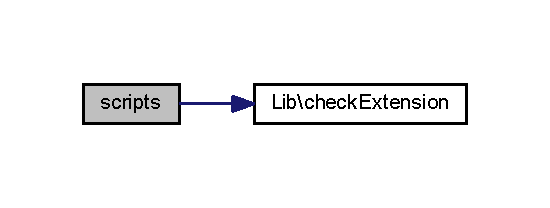
\includegraphics[width=264pt]{class_lora_1_1_page_component_a3dc593f496b7dbf2e5e3c406cb5fd106_cgraph}
\end{center}
\end{figure}
\mbox{\label{class_lora_1_1_page_component_a53d31780f290c90071a213e9f786abb3}} 
\index{Lora\+::\+Page\+Component@{Lora\+::\+Page\+Component}!styles@{styles}}
\index{styles@{styles}!Lora\+::\+Page\+Component@{Lora\+::\+Page\+Component}}
\subsubsection{styles()}
{\footnotesize\ttfamily styles (\begin{DoxyParamCaption}{ }\end{DoxyParamCaption})}

Returns an array containing all styles assigned to this component. Goes through all of them and adds file extension to them if needed. \begin{DoxyReturn}{Returns}
Returns an array of file names. 
\end{DoxyReturn}

\begin{DoxyCode}
124                               : array \{
125         \textcolor{keywordflow}{foreach} ($this->\_styles as &$style) \{
126             $style = \Lib::checkExtension ($style, \textcolor{stringliteral}{'css'});
127         \} \textcolor{keywordflow}{return} $this->\_styles;
128     \}
\end{DoxyCode}
Here is the call graph for this function\+:\nopagebreak
\begin{figure}[H]
\begin{center}
\leavevmode
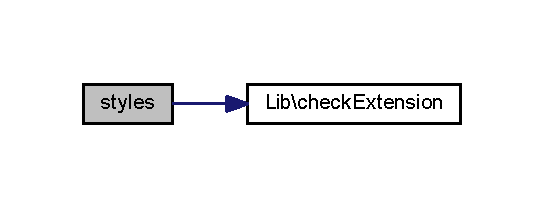
\includegraphics[width=261pt]{class_lora_1_1_page_component_a53d31780f290c90071a213e9f786abb3_cgraph}
\end{center}
\end{figure}
\mbox{\label{class_lora_1_1_page_component_a0b54c9d3801b331b75487ef78d98c06b}} 
\index{Lora\+::\+Page\+Component@{Lora\+::\+Page\+Component}!template@{template}}
\index{template@{template}!Lora\+::\+Page\+Component@{Lora\+::\+Page\+Component}}
\subsubsection{template()}
{\footnotesize\ttfamily template (\begin{DoxyParamCaption}{ }\end{DoxyParamCaption})}

\begin{DoxyReturn}{Returns}
Returns a template file name this \doxyref{Page\+Component}{p.}{class_lora_1_1_page_component} uses and adds file extension to it if required. 
\end{DoxyReturn}

\begin{DoxyCode}
73                                 : \textcolor{keywordtype}{string} \{
74         \textcolor{keywordflow}{return} $this->\_template = \Lib::checkExtension ($this->\_template, 
      Config::ext (\textcolor{stringliteral}{'twig'}, \textcolor{stringliteral}{'twig'}));
75     \}
\end{DoxyCode}
Here is the call graph for this function\+:\nopagebreak
\begin{figure}[H]
\begin{center}
\leavevmode
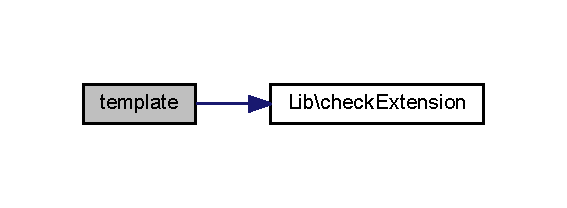
\includegraphics[width=272pt]{class_lora_1_1_page_component_a0b54c9d3801b331b75487ef78d98c06b_cgraph}
\end{center}
\end{figure}


The documentation for this class was generated from the following file\+:\begin{DoxyCompactItemize}
\item 
servers/webserver/server/pagecomponent.\+php\end{DoxyCompactItemize}

\hypertarget{class_lora_1_1_page_manager}{}\section{Page\+Manager Class Reference}
\label{class_lora_1_1_page_manager}\index{Page\+Manager@{Page\+Manager}}
\subsection*{Public Member Functions}
\begin{DoxyCompactItemize}
\item 
\mbox{\Hypertarget{class_lora_1_1_page_manager_ad3e2c2ddb1a0601061eadd0d48404fd0}\label{class_lora_1_1_page_manager_ad3e2c2ddb1a0601061eadd0d48404fd0}} 
{\bfseries cache} (\hyperlink{class_lora_1_1_page}{Page} \$page, string \$id)
\item 
\mbox{\Hypertarget{class_lora_1_1_page_manager_a766144b3d568ea2b61e4432c62da9dee}\label{class_lora_1_1_page_manager_a766144b3d568ea2b61e4432c62da9dee}} 
{\bfseries load} (\hyperlink{class_lora_1_1_base_action}{Base\+Action} \$action)
\end{DoxyCompactItemize}
\subsection*{Data Fields}
\begin{DoxyCompactItemize}
\item 
\mbox{\Hypertarget{class_lora_1_1_page_manager_a7741f32e8202cda9b33453211d3c18f3}\label{class_lora_1_1_page_manager_a7741f32e8202cda9b33453211d3c18f3}} 
{\bfseries \$cache\+Enabled} = false
\end{DoxyCompactItemize}
\subsection*{Private Attributes}
\begin{DoxyCompactItemize}
\item 
\mbox{\Hypertarget{class_lora_1_1_page_manager_a0a4baf0b22973c07685c3981f0d17fc4}\label{class_lora_1_1_page_manager_a0a4baf0b22973c07685c3981f0d17fc4}} 
{\bfseries \$path} = \char`\"{}\char`\"{}
\end{DoxyCompactItemize}


The documentation for this class was generated from the following file\+:\begin{DoxyCompactItemize}
\item 
servers/webserver/server/managers/pagemanager.\+php\end{DoxyCompactItemize}

\hypertarget{class_lora_1_1_page_view}{}\section{Page\+View Class Reference}
\label{class_lora_1_1_page_view}\index{Page\+View@{Page\+View}}
\subsection*{Public Member Functions}
\begin{DoxyCompactItemize}
\item 
\hyperlink{class_lora_1_1_page_view_af90bbf86e6056724a44e281fb7125565}{\+\_\+\+\_\+construct} (string \$name=\textquotesingle{}\textquotesingle{})
\item 
\hyperlink{class_lora_1_1_page_view_a476c28dc9ec4f9be50d2e19ad74f4a06}{link} (\hyperlink{class_lora_1_1_page}{Page} \$page, string \$text)
\item 
\hyperlink{class_lora_1_1_page_view_a14fdcc82bbf2c7647e9c6821a2227a1f}{show} (bool \$show=null)
\item 
\hyperlink{class_lora_1_1_page_view_a087060b582403885d08e89ad894ecc5d}{id} ()
\item 
\hyperlink{class_lora_1_1_page_view_a3178ecfe82b87d56467cd68c74300201}{set\+Layout} (string \$\hyperlink{class_lora_1_1_page_view_a0e9447221830f8629717836bd933a164}{layout})
\item 
\hyperlink{class_lora_1_1_page_view_a0e9447221830f8629717836bd933a164}{layout} ()
\item 
\hyperlink{class_lora_1_1_page_view_a9b80bb36f89498eac4f43bf08461240d}{content} ()
\item 
\hyperlink{class_lora_1_1_page_view_aa3b783aa411b948184d94c54f1b5e2b3}{add\+Component} (string \$component\+Name)
\item 
\hyperlink{class_lora_1_1_page_view_abed72eecd6815f748031505225cc1319}{components} ()
\item 
\hyperlink{class_lora_1_1_page_view_a2cb0c3fbaa3e77419479aef9716f1ce3}{load} (array \$config)
\end{DoxyCompactItemize}
\subsection*{Data Fields}
\begin{DoxyCompactItemize}
\item 
\mbox{\Hypertarget{class_lora_1_1_page_view_a1a9789c0b0363f3e9c69c9d0659497cc}\label{class_lora_1_1_page_view_a1a9789c0b0363f3e9c69c9d0659497cc}} 
{\bfseries \$\+\_\+sub\+\_\+layout} = \textquotesingle{}\textquotesingle{}
\item 
\mbox{\Hypertarget{class_lora_1_1_page_view_a921d8b4050e6b39e1507f14dea363ebf}\label{class_lora_1_1_page_view_a921d8b4050e6b39e1507f14dea363ebf}} 
{\bfseries \$\+\_\+content} = \textquotesingle{}\textquotesingle{}
\item 
\mbox{\Hypertarget{class_lora_1_1_page_view_a2409c247baf67a1d4c6b9a1789cfc088}\label{class_lora_1_1_page_view_a2409c247baf67a1d4c6b9a1789cfc088}} 
{\bfseries \$components} = \mbox{[}$\,$\mbox{]}
\item 
\mbox{\Hypertarget{class_lora_1_1_page_view_a393fcb2f39dd1ec57feb8c377fd1c22e}\label{class_lora_1_1_page_view_a393fcb2f39dd1ec57feb8c377fd1c22e}} 
{\bfseries \$visible} = false
\item 
\mbox{\Hypertarget{class_lora_1_1_page_view_a5d346e31b75d916e3bac9cb193bfc97f}\label{class_lora_1_1_page_view_a5d346e31b75d916e3bac9cb193bfc97f}} 
{\bfseries \$link} = null
\end{DoxyCompactItemize}
\subsection*{Private Member Functions}
\begin{DoxyCompactItemize}
\item 
\hyperlink{class_lora_1_1_page_view_a3b38056ae9a3c2cada8000895f46b9cb}{configurable\+Fields} (array \$exclude=\mbox{[}$\,$\mbox{]})
\item 
\hyperlink{class_lora_1_1_page_view_a63ba1656485acf76a0d23e8f64fdfa1d}{parse\+File} (string \$file)
\end{DoxyCompactItemize}
\subsection*{Private Attributes}
\begin{DoxyCompactItemize}
\item 
\mbox{\Hypertarget{class_lora_1_1_page_view_a1c89defaf5aa7ac8e526065e8572f580}\label{class_lora_1_1_page_view_a1c89defaf5aa7ac8e526065e8572f580}} 
{\bfseries \$\+\_\+name} = \textquotesingle{}\textquotesingle{}
\end{DoxyCompactItemize}


\subsection{Detailed Description}
A subview for page. Subview may have 0 to n Page\+Components (or components for short when talking about pages) assigned to them. These components are added to the page by Twig. This class might later be moved to  -\/namespace. 

\subsection{Constructor \& Destructor Documentation}
\mbox{\Hypertarget{class_lora_1_1_page_view_af90bbf86e6056724a44e281fb7125565}\label{class_lora_1_1_page_view_af90bbf86e6056724a44e281fb7125565}} 
\index{Lora\+::\+Page\+View@{Lora\+::\+Page\+View}!\+\_\+\+\_\+construct@{\+\_\+\+\_\+construct}}
\index{\+\_\+\+\_\+construct@{\+\_\+\+\_\+construct}!Lora\+::\+Page\+View@{Lora\+::\+Page\+View}}
\subsubsection{\texorpdfstring{\+\_\+\+\_\+construct()}{\_\_construct()}}
{\footnotesize\ttfamily \+\_\+\+\_\+construct (\begin{DoxyParamCaption}\item[{string}]{\$name = {\ttfamily \textquotesingle{}\textquotesingle{}} }\end{DoxyParamCaption})}


\begin{DoxyParams}{Parameters}
{\em \$name} & Name of this \hyperlink{class_lora_1_1_page_view}{Page\+View} \\
\hline
\end{DoxyParams}

\begin{DoxyCode}
24                                                     \{
25         $this->\_name = $name;
26     \}
\end{DoxyCode}


\subsection{Member Function Documentation}
\mbox{\Hypertarget{class_lora_1_1_page_view_aa3b783aa411b948184d94c54f1b5e2b3}\label{class_lora_1_1_page_view_aa3b783aa411b948184d94c54f1b5e2b3}} 
\index{Lora\+::\+Page\+View@{Lora\+::\+Page\+View}!add\+Component@{add\+Component}}
\index{add\+Component@{add\+Component}!Lora\+::\+Page\+View@{Lora\+::\+Page\+View}}
\subsubsection{\texorpdfstring{add\+Component()}{addComponent()}}
{\footnotesize\ttfamily add\+Component (\begin{DoxyParamCaption}\item[{string}]{\$component\+Name }\end{DoxyParamCaption})}

Adds a new component to this \hyperlink{class_lora_1_1_page_view}{Page\+View} if such exist. 
\begin{DoxyParams}{Parameters}
{\em \$component\+Name} & Name of the Page\+Componet which is wished to be added to this \hyperlink{class_lora_1_1_page_view}{Page\+View}. \\
\hline
\end{DoxyParams}

\begin{DoxyCode}
82                                                          : \textcolor{keywordtype}{void} \{
83         \textcolor{keywordflow}{if} (($comp = \hyperlink{class_lora_1_1_page_component_ab6c03d0ec66cb31bfc74a784387cef33}{PageComponent::Create} ($componentName)) !== null) \{
84             $this->\hyperlink{class_lora_1_1_page_view_abed72eecd6815f748031505225cc1319}{components} [] = $comp;
85         \}
86     \}
\end{DoxyCode}
\mbox{\Hypertarget{class_lora_1_1_page_view_abed72eecd6815f748031505225cc1319}\label{class_lora_1_1_page_view_abed72eecd6815f748031505225cc1319}} 
\index{Lora\+::\+Page\+View@{Lora\+::\+Page\+View}!components@{components}}
\index{components@{components}!Lora\+::\+Page\+View@{Lora\+::\+Page\+View}}
\subsubsection{\texorpdfstring{components()}{components()}}
{\footnotesize\ttfamily components (\begin{DoxyParamCaption}{ }\end{DoxyParamCaption})}

\begin{DoxyReturn}{Returns}
Returns an array containing all components of this view. 
\end{DoxyReturn}

\begin{DoxyCode}
91                                   : array \{
92         \textcolor{keywordflow}{return} $this->components;
93     \}
\end{DoxyCode}
\mbox{\Hypertarget{class_lora_1_1_page_view_a3b38056ae9a3c2cada8000895f46b9cb}\label{class_lora_1_1_page_view_a3b38056ae9a3c2cada8000895f46b9cb}} 
\index{Lora\+::\+Page\+View@{Lora\+::\+Page\+View}!configurable\+Fields@{configurable\+Fields}}
\index{configurable\+Fields@{configurable\+Fields}!Lora\+::\+Page\+View@{Lora\+::\+Page\+View}}
\subsubsection{\texorpdfstring{configurable\+Fields()}{configurableFields()}}
{\footnotesize\ttfamily configurable\+Fields (\begin{DoxyParamCaption}\item[{array}]{\$exclude = {\ttfamily \mbox{[}\mbox{]}} }\end{DoxyParamCaption})\hspace{0.3cm}{\ttfamily [private]}}

Returns an array of property field names in this class which can be set using initialization files with \hyperlink{class_lora_1_1_page_view_a2cb0c3fbaa3e77419479aef9716f1ce3}{Page\+View\+::load}. 
\begin{DoxyParams}{Parameters}
{\em \$exclude} & An array containing field names which are to be excluded from the final collection. \\
\hline
\end{DoxyParams}
\begin{DoxyReturn}{Returns}
Returns an array of field names. It is possible for this array to be empty. 
\end{DoxyReturn}

\begin{DoxyCode}
121                                                               : array \{
122         \textcolor{keywordflow}{return} array\_filter (
123             array\_map (\textcolor{keyword}{function} ($field) \{ \textcolor{keywordflow}{return} $field->name; \}, (new \(\backslash\)ReflectionClass ($this))->
      getProperties ()),
124             \textcolor{keyword}{function} ($field) use ($exclude) \{
125                 \textcolor{keywordflow}{return} @$field [0] === \textcolor{charliteral}{'\_'} && !in\_array ($field, $exclude); \}
126         );
127     \}
\end{DoxyCode}
\mbox{\Hypertarget{class_lora_1_1_page_view_a9b80bb36f89498eac4f43bf08461240d}\label{class_lora_1_1_page_view_a9b80bb36f89498eac4f43bf08461240d}} 
\index{Lora\+::\+Page\+View@{Lora\+::\+Page\+View}!content@{content}}
\index{content@{content}!Lora\+::\+Page\+View@{Lora\+::\+Page\+View}}
\subsubsection{\texorpdfstring{content()}{content()}}
{\footnotesize\ttfamily content (\begin{DoxyParamCaption}{ }\end{DoxyParamCaption})}

\begin{DoxyReturn}{Returns}
Returns the name of the file containing this \hyperlink{class_lora_1_1_page_view}{Page\+View}\textquotesingle{}s content and adds extension to it if one does not exist. 
\end{DoxyReturn}

\begin{DoxyCode}
74                                : \textcolor{keywordtype}{string} \{
75         \textcolor{keywordflow}{return} $this->\_content = \hyperlink{class_lib_ab5fbdf394f09fcef4dcea271c344cb65}{\(\backslash\)Lib::checkExtension} ($this->\_content, 
      \hyperlink{class_lora_1_1_config_a98a88f17bbc72a1f26f54b264be26068}{Config::ext} (\textcolor{stringliteral}{'twig'}, \textcolor{stringliteral}{'twig'}));
76     \}
\end{DoxyCode}
Here is the call graph for this function\+:
% FIG 0
\mbox{\Hypertarget{class_lora_1_1_page_view_a087060b582403885d08e89ad894ecc5d}\label{class_lora_1_1_page_view_a087060b582403885d08e89ad894ecc5d}} 
\index{Lora\+::\+Page\+View@{Lora\+::\+Page\+View}!id@{id}}
\index{id@{id}!Lora\+::\+Page\+View@{Lora\+::\+Page\+View}}
\subsubsection{\texorpdfstring{id()}{id()}}
{\footnotesize\ttfamily id (\begin{DoxyParamCaption}{ }\end{DoxyParamCaption})}

\begin{DoxyRefDesc}{Todo}
\item[\hyperlink{todo__todo000009}{Todo}]This method should be renamed to \textquotesingle{}name\textquotesingle{}. \end{DoxyRefDesc}
\begin{DoxyReturn}{Returns}
Returns the name of this view. 
\end{DoxyReturn}

\begin{DoxyCode}
52                           \{
53         \textcolor{keywordflow}{return} $this->\_name;
54     \}
\end{DoxyCode}
Here is the caller graph for this function\+:
% FIG 1
\mbox{\Hypertarget{class_lora_1_1_page_view_a0e9447221830f8629717836bd933a164}\label{class_lora_1_1_page_view_a0e9447221830f8629717836bd933a164}} 
\index{Lora\+::\+Page\+View@{Lora\+::\+Page\+View}!layout@{layout}}
\index{layout@{layout}!Lora\+::\+Page\+View@{Lora\+::\+Page\+View}}
\subsubsection{\texorpdfstring{layout()}{layout()}}
{\footnotesize\ttfamily layout (\begin{DoxyParamCaption}{ }\end{DoxyParamCaption})}

\begin{DoxyReturn}{Returns}
Returns the name of the file containing this \hyperlink{class_lora_1_1_page_view}{Page\+View}\textquotesingle{}s layout and adds extension to it if one does not exist. 
\end{DoxyReturn}

\begin{DoxyCode}
67                               : \textcolor{keywordtype}{string} \{
68         \textcolor{keywordflow}{return} $this->\_sub\_layout = \hyperlink{class_lib_ab5fbdf394f09fcef4dcea271c344cb65}{\(\backslash\)Lib::checkExtension} ($this->\_sub\_layout, 
      \hyperlink{class_lora_1_1_config_a98a88f17bbc72a1f26f54b264be26068}{Config::ext} (\textcolor{stringliteral}{'twig'}, \textcolor{stringliteral}{'twig'}));
69     \}
\end{DoxyCode}
Here is the call graph for this function\+:
% FIG 2
\mbox{\Hypertarget{class_lora_1_1_page_view_a476c28dc9ec4f9be50d2e19ad74f4a06}\label{class_lora_1_1_page_view_a476c28dc9ec4f9be50d2e19ad74f4a06}} 
\index{Lora\+::\+Page\+View@{Lora\+::\+Page\+View}!link@{link}}
\index{link@{link}!Lora\+::\+Page\+View@{Lora\+::\+Page\+View}}
\subsubsection{\texorpdfstring{link()}{link()}}
{\footnotesize\ttfamily link (\begin{DoxyParamCaption}\item[{\hyperlink{class_lora_1_1_page}{Page}}]{\$page,  }\item[{string}]{\$text }\end{DoxyParamCaption})}

Generates an  object to this view. 
\begin{DoxyParams}{Parameters}
{\em \$page} & The page to which this view belongs to. This might be removed in the future if Page\+Views are made aware of their containing \hyperlink{class_lora_1_1_page}{Page}. \\
\hline
{\em \$text} & Visible text of the link. \\
\hline
\end{DoxyParams}

\begin{DoxyCode}
33                                                     \{
34         \textcolor{keywordflow}{return} $this->\hyperlink{class_lora_1_1_page_view_a476c28dc9ec4f9be50d2e19ad74f4a06}{link} ?? $this->\hyperlink{class_lora_1_1_page_view_a476c28dc9ec4f9be50d2e19ad74f4a06}{link} = new \(\backslash\)Html\(\backslash\)Link ($text, $page->name (), [ $this->\_name =
      > \textcolor{stringliteral}{''} ], [ \textcolor{stringliteral}{'data-view-name'} => $this->\_name ]);
35     \}
\end{DoxyCode}
Here is the call graph for this function\+:
% FIG 3
\mbox{\Hypertarget{class_lora_1_1_page_view_a2cb0c3fbaa3e77419479aef9716f1ce3}\label{class_lora_1_1_page_view_a2cb0c3fbaa3e77419479aef9716f1ce3}} 
\index{Lora\+::\+Page\+View@{Lora\+::\+Page\+View}!load@{load}}
\index{load@{load}!Lora\+::\+Page\+View@{Lora\+::\+Page\+View}}
\subsubsection{\texorpdfstring{load()}{load()}}
{\footnotesize\ttfamily load (\begin{DoxyParamCaption}\item[{array}]{\$config }\end{DoxyParamCaption})}

Reads preoperty values for this instance from an array. Capable of creating new \hyperlink{class_lora_1_1_page_component}{Page\+Component} instances by name. 
\begin{DoxyParams}{Parameters}
{\em \$config} & An array containing property values for this object. \\
\hline
\end{DoxyParams}

\begin{DoxyCode}
100                                          : \textcolor{keywordtype}{void} \{
101         \textcolor{keywordflow}{foreach} ($this->\hyperlink{class_lora_1_1_page_view_a3b38056ae9a3c2cada8000895f46b9cb}{configurableFields} () as $member) \{
102             $property = substr ($member, 1);
103             \textcolor{keywordflow}{if} (isset ($config [$property]) && gettype ($config [$property]) === gettype ($this->$member)) 
      \{
104                 $this->$member = $config [$property];
105             \}
106         \}
107         \textcolor{keywordflow}{if} (isset ($config [\textcolor{stringliteral}{'components'}]) && is\_array ($config [\textcolor{stringliteral}{'components'}])) \{
108             \textcolor{keywordflow}{foreach} ($config [\textcolor{stringliteral}{'components'}] as $comp) \{
109                 \textcolor{keywordflow}{if} (gettype ($comp) === \textcolor{stringliteral}{"string"}) \{
110                     $this->\hyperlink{class_lora_1_1_page_view_aa3b783aa411b948184d94c54f1b5e2b3}{addComponent} ($comp);
111                 \}
112             \}
113         \}
114     \}
\end{DoxyCode}
\mbox{\Hypertarget{class_lora_1_1_page_view_a63ba1656485acf76a0d23e8f64fdfa1d}\label{class_lora_1_1_page_view_a63ba1656485acf76a0d23e8f64fdfa1d}} 
\index{Lora\+::\+Page\+View@{Lora\+::\+Page\+View}!parse\+File@{parse\+File}}
\index{parse\+File@{parse\+File}!Lora\+::\+Page\+View@{Lora\+::\+Page\+View}}
\subsubsection{\texorpdfstring{parse\+File()}{parseFile()}}
{\footnotesize\ttfamily parse\+File (\begin{DoxyParamCaption}\item[{string}]{\$file }\end{DoxyParamCaption})\hspace{0.3cm}{\ttfamily [private]}}

Reads in a value file containing property values for this object. Not in use. 
\begin{DoxyParams}{Parameters}
{\em \$file} & Full path of the file containing property values. Can be an I\+NI or J\+S\+ON file. \\
\hline
\end{DoxyParams}
\begin{DoxyReturn}{Returns}
Returns an array of property values on success or an empty array on failure. 
\end{DoxyReturn}

\begin{DoxyCode}
135                                               : array \{
136         \textcolor{keywordflow}{if} (empty ($config = @parse\_ini\_file ($file, \textcolor{keyword}{true}, INI\_SCANNER\_TYPED)) && empty ($config = @
      json\_decode (file\_get\_contents ($file), \textcolor{keyword}{true}))) \{
137             \textcolor{keywordflow}{return} [];
138         \}
139         \textcolor{keywordflow}{return} $config;
140     \}
\end{DoxyCode}
\mbox{\Hypertarget{class_lora_1_1_page_view_a3178ecfe82b87d56467cd68c74300201}\label{class_lora_1_1_page_view_a3178ecfe82b87d56467cd68c74300201}} 
\index{Lora\+::\+Page\+View@{Lora\+::\+Page\+View}!set\+Layout@{set\+Layout}}
\index{set\+Layout@{set\+Layout}!Lora\+::\+Page\+View@{Lora\+::\+Page\+View}}
\subsubsection{\texorpdfstring{set\+Layout()}{setLayout()}}
{\footnotesize\ttfamily set\+Layout (\begin{DoxyParamCaption}\item[{string}]{\$layout }\end{DoxyParamCaption})}

An unused feature but it is possible to define a layout for views. 
\begin{DoxyParams}{Parameters}
{\em \$layout} & Name of a layout file for this view with or without extension. \\
\hline
\end{DoxyParams}

\begin{DoxyCode}
60                                                : \textcolor{keywordtype}{void} \{
61         $this->\_sub\_layout = $layout;
62     \}
\end{DoxyCode}
\mbox{\Hypertarget{class_lora_1_1_page_view_a14fdcc82bbf2c7647e9c6821a2227a1f}\label{class_lora_1_1_page_view_a14fdcc82bbf2c7647e9c6821a2227a1f}} 
\index{Lora\+::\+Page\+View@{Lora\+::\+Page\+View}!show@{show}}
\index{show@{show}!Lora\+::\+Page\+View@{Lora\+::\+Page\+View}}
\subsubsection{\texorpdfstring{show()}{show()}}
{\footnotesize\ttfamily show (\begin{DoxyParamCaption}\item[{bool}]{\$show = {\ttfamily null} }\end{DoxyParamCaption})}

If \$show is defined, the \$visible property is set to value of \$show. If not, this method return \$visible property value. 
\begin{DoxyParams}{Parameters}
{\em \$show} & An optional boolean value to determine if this view is visible or not. \\
\hline
\end{DoxyParams}
\begin{DoxyReturn}{Returns}
Returns a boolean determining this view\textquotesingle{}s visibility. 
\end{DoxyReturn}

\begin{DoxyCode}
42                                              \{
43         \textcolor{keywordflow}{if} ($show === null) \{
44             \textcolor{keywordflow}{return} $this->visible;
45         \} $this->visible = $show;
46     \}
\end{DoxyCode}


The documentation for this class was generated from the following file\+:\begin{DoxyCompactItemize}
\item 
servers/webserver/server/pageview.\+php\end{DoxyCompactItemize}

\section{Realtime\+Server Class Reference}
\label{class_lora_1_1_realtime_server}\index{Realtime\+Server@{Realtime\+Server}}


Inheritance diagram for Realtime\+Server\+:
\nopagebreak
\begin{figure}[H]
\begin{center}
\leavevmode
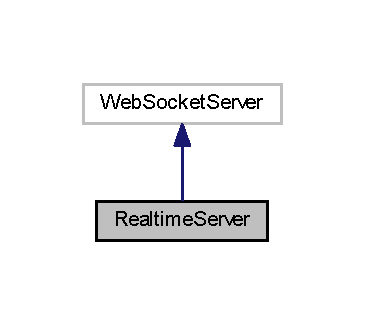
\includegraphics[width=175pt]{class_lora_1_1_realtime_server__inherit__graph}
\end{center}
\end{figure}


Collaboration diagram for Realtime\+Server\+:
\nopagebreak
\begin{figure}[H]
\begin{center}
\leavevmode
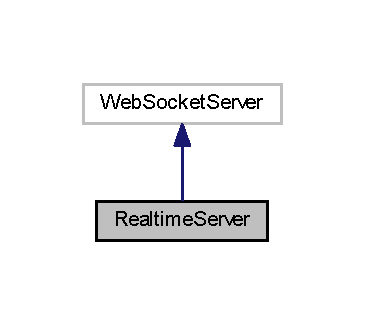
\includegraphics[width=175pt]{class_lora_1_1_realtime_server__coll__graph}
\end{center}
\end{figure}
\subsection*{Public Member Functions}
\begin{DoxyCompactItemize}
\item 
\mbox{\label{class_lora_1_1_realtime_server_a473114c92843eda7de537f42ffde8913}} 
{\bfseries broadcast} (string \$msg)
\end{DoxyCompactItemize}
\subsection*{Protected Member Functions}
\begin{DoxyCompactItemize}
\item 
\mbox{\label{class_lora_1_1_realtime_server_a805b6933fa0b69978e35fe94f3884de7}} 
{\bfseries process} (\$user, \$message)
\item 
\mbox{\label{class_lora_1_1_realtime_server_a3e89014762456a67edbe843811c78736}} 
{\bfseries connected} (\$user)
\item 
\mbox{\label{class_lora_1_1_realtime_server_aaf6375ec8ee41584a5adcf3d85d73018}} 
{\bfseries closed} (\$user)
\end{DoxyCompactItemize}


The documentation for this class was generated from the following file\+:\begin{DoxyCompactItemize}
\item 
servers/rtserver/server/realtimeserver.\+php\end{DoxyCompactItemize}

\section{Request\+Data Class Reference}
\label{class_request_data}\index{Request\+Data@{Request\+Data}}
\subsection*{Public Member Functions}
\begin{DoxyCompactItemize}
\item 
\mbox{\label{class_request_data_a669382ca8209546c1fc5b69805e246b8}} 
{\bfseries \+\_\+\+\_\+construct} (\$request\+\_\+data)
\item 
\mbox{\label{class_request_data_a8b23dbb48f0c3c94725695191d06981a}} 
{\bfseries has} (\$key)
\item 
\mbox{\label{class_request_data_afc5fb78e5e7b38a63f47c60d59b76083}} 
{\bfseries read\+Int} (\$key, \&\$value, \$default=null)
\item 
\mbox{\label{class_request_data_a4195c2ac041f755cc109d09db8ca856f}} 
{\bfseries read\+Bool} (\$key, \&\$value, \$default=null)
\item 
\mbox{\label{class_request_data_ac63931fd6da0fd43e2a5ec496d5dfec5}} 
{\bfseries read\+String} (\$key, \&\$value, \$default=null)
\item 
\mbox{\label{class_request_data_a829933c7b0b8ddb5c59e7e23b1bb970d}} 
{\bfseries read\+Array} (\$key, \&\$value, \$default=[$\,$])
\item 
\mbox{\label{class_request_data_aa66e1367f11839054f97149dbfdddc12}} 
{\bfseries get\+Int} (\$key, \$default=null)
\item 
\mbox{\label{class_request_data_a19e53a2778353bd321daf84c70131a09}} 
{\bfseries get\+Bool} (\$key, \$default=null)
\item 
\mbox{\label{class_request_data_a05d694eeb9f165bd8e0245c06a34a807}} 
{\bfseries get\+String} (\$key, \$default=null)
\item 
\mbox{\label{class_request_data_af06da642a5e374ae44f35473971fe117}} 
{\bfseries get\+Array} (\$key, \$default=null)
\item 
\mbox{\label{class_request_data_a853b5161c2de226a00f31fb6dfcbd93d}} 
{\bfseries get\+Int\+Array} (array \$keys)
\item 
\mbox{\label{class_request_data_ad00cd3a1c703f0a7e2df35d873b3fd01}} 
{\bfseries get\+Bool\+Array} (array \$keys)
\item 
\mbox{\label{class_request_data_a0566129c074d52a4db99520e7092b68c}} 
{\bfseries get\+String\+Array} (array \$keys)
\item 
\mbox{\label{class_request_data_a9197f1583e1ad33cbd28fbc10b339fb5}} 
{\bfseries get\+Array\+Array} (array \$keys)
\end{DoxyCompactItemize}
\subsection*{Private Member Functions}
\begin{DoxyCompactItemize}
\item 
\textbf{ get\+Typed\+Array} (array \$keys, string \$method)
\end{DoxyCompactItemize}
\subsection*{Private Attributes}
\begin{DoxyCompactItemize}
\item 
\mbox{\label{class_request_data_a6efc15b5a2314dd4b5aaa556a375c6d6}} 
{\bfseries \$data} = [$\,$]
\end{DoxyCompactItemize}


\subsection{Detailed Description}
A wrapper for request data arriving from client side. Makes it easier to safely read typed values. Another benefit is that since reuest parameters no longer needn\textquotesingle{}t to be passed around as an array, the parameter array isn\textquotesingle{}t copied on every method call. Might make code cleaner too.
\begin{DoxyItemize}
\item Most definitely makes code cleaner.
\end{DoxyItemize}

Each read -\/method returns true, if the value conversion succeeded and false in case of failure. \$value is set to default in case of failure.

get -\/methods return either the requested value or default value. Was added to allow cleaner use.

get\+T\+Array -\/methods read multiple values with the key array they take as a parameter. One default value can be defined which will be assigned to any missing values.

N\+O\+T\+E! Values read using this class must still be checked for proper value ranges. Take especial care with strings since they are rather complex to verify in some cases.

N\+O\+T\+E! String methods in this class can be used to fetch integer and floating point values as well. If you need to get mixed values, use the string methods. Do note that arrays cannot be fetched using string methods since P\+HP raises a notice from converting an array to string.

T\+O\+DO\+: Research how casting the values to their corresponding types would affect the output.
\begin{DoxyItemize}
\item Int casting can be done.
\end{DoxyItemize}

M\+E\+MO\+: If optimization is required, look into filter\+\_\+var\+\_\+array

\begin{DoxyVerb}NOTE! ONE MUST NOT add a method which allows direct access to $data -array since that   *
        invalidates the whole point of having this class in the first place.            *
\end{DoxyVerb}


\begin{DoxyRefDesc}{Todo}
\item[\textbf{ Todo}]Write type checks for default values and resolve to null if they are of incorrect type. \end{DoxyRefDesc}


\subsection{Member Function Documentation}
\mbox{\label{class_request_data_aad8cc8d83c11936ce64f708392057942}} 
\index{Request\+Data@{Request\+Data}!get\+Typed\+Array@{get\+Typed\+Array}}
\index{get\+Typed\+Array@{get\+Typed\+Array}!Request\+Data@{Request\+Data}}
\subsubsection{get\+Typed\+Array()}
{\footnotesize\ttfamily get\+Typed\+Array (\begin{DoxyParamCaption}\item[{array}]{\$keys,  }\item[{string}]{\$method }\end{DoxyParamCaption})\hspace{0.3cm}{\ttfamily [private]}}

Returns an array with its keys set to provided ones. Values are fetched from \$data under same keys. If no entry is found for a key, the value is set to default. 
\begin{DoxyCode}
131                                                                  : ?array \{
132         $values = [];
133         \textcolor{keywordflow}{foreach} ($keys as $key => $value) \{
134             $values [$key] = $this->$method ($key, $value);
135         \} \textcolor{keywordflow}{return} $values;
136     \}
\end{DoxyCode}


The documentation for this class was generated from the following file\+:\begin{DoxyCompactItemize}
\item 
lora/util/requestdata.\+php\end{DoxyCompactItemize}

\section{Request\+Handler Class Reference}
\label{class_lora_1_1_request_handler}\index{Request\+Handler@{Request\+Handler}}
\subsection*{Public Member Functions}
\begin{DoxyCompactItemize}
\item 
\textbf{ \+\_\+\+\_\+construct} (\textbackslash{}Slim\textbackslash{}\+Slim \$slim)
\item 
\textbf{ handle\+Content\+Request} (array \$action)
\item 
\textbf{ handle\+Api\+Request} (array \$action)
\end{DoxyCompactItemize}
\subsection*{Data Fields}
\begin{DoxyCompactItemize}
\item 
\mbox{\label{class_lora_1_1_request_handler_a63a7a283ea5dee8af1e2d5a3435bf370}} 
{\bfseries \$req} = null
\item 
\mbox{\label{class_lora_1_1_request_handler_a7402b7f726abbbfe8793e75fafcd5e91}} 
{\bfseries \$mess} = null
\item 
\mbox{\label{class_lora_1_1_request_handler_a0a44e6760141442bb439b1ab1395d8ff}} 
{\bfseries \$page} = null
\item 
\mbox{\label{class_lora_1_1_request_handler_a0002d5f2a35dc15ffc92761388fd9bb8}} 
{\bfseries \$pm} = null
\item 
\mbox{\label{class_lora_1_1_request_handler_a12661b2fc0f57f97e30a1620889ce9c6}} 
{\bfseries \$method} = \textquotesingle{}\textquotesingle{}
\item 
\mbox{\label{class_lora_1_1_request_handler_ab37f7c32f41c3c61ed940887453767f4}} 
{\bfseries \$root} = \textquotesingle{}\textquotesingle{}
\end{DoxyCompactItemize}
\subsection*{Private Member Functions}
\begin{DoxyCompactItemize}
\item 
\textbf{ resolve\+Call} (array \$action, string \$file\+Path, string \$file\+Type, string \$namespace)
\item 
\textbf{ not\+Found} (array \&\$consumed, string \&\$path, string \$folder)
\item 
\textbf{ action\+To\+Path} (array \$action, array \&\$consumed, array \&\$excess, string \&\$path, string \$folder)
\item 
\textbf{ build\+Page} ()
\item 
\textbf{ default\+Visibility} ()
\item 
\textbf{ build\+Class\+Name} (array \$action, string \&\$class, string \&\$plain\+Name, string \$prefix, string \$namespace)
\item 
\textbf{ load\+File} (string \$path)
\end{DoxyCompactItemize}
\subsection*{Private Attributes}
\begin{DoxyCompactItemize}
\item 
\mbox{\label{class_lora_1_1_request_handler_acfcdba42d947eb8c034b44898adda679}} 
{\bfseries \$slim} = null
\end{DoxyCompactItemize}


\subsection{Detailed Description}
A class which processes every request coming to this web server. 

\subsection{Constructor \& Destructor Documentation}
\mbox{\label{class_lora_1_1_request_handler_ae94f71807587d45d185150087e3c313d}} 
\index{Lora\+::\+Request\+Handler@{Lora\+::\+Request\+Handler}!\+\_\+\+\_\+construct@{\+\_\+\+\_\+construct}}
\index{\+\_\+\+\_\+construct@{\+\_\+\+\_\+construct}!Lora\+::\+Request\+Handler@{Lora\+::\+Request\+Handler}}
\subsubsection{\+\_\+\+\_\+construct()}
{\footnotesize\ttfamily \+\_\+\+\_\+construct (\begin{DoxyParamCaption}\item[{\textbackslash{}Slim\textbackslash{}\+Slim}]{\$slim }\end{DoxyParamCaption})}

$<$ Convert H\+T\+TP method into a \doxyref{Base\+Action}{p.}{class_lora_1_1_base_action} method name. 
\begin{DoxyCode}
21                                                    \{
22         $this->slim         = $slim;
23         $this->method       = \textcolor{charliteral}{'\_'}.strtolower ($this->slim->request->getMethod ()); 
24         $this->req          = new \(\backslash\)RequestData ($this->slim->request->params ());
25         $this->mess         = \textcolor{keyword}{new} Messenger ();
26         $this->root         = Config::path (\textcolor{stringliteral}{'server'}, \textcolor{stringliteral}{'root'});
27     \}
\end{DoxyCode}


\subsection{Member Function Documentation}
\mbox{\label{class_lora_1_1_request_handler_a9b2ad6505d2d31b163bc604a408b9d54}} 
\index{Lora\+::\+Request\+Handler@{Lora\+::\+Request\+Handler}!action\+To\+Path@{action\+To\+Path}}
\index{action\+To\+Path@{action\+To\+Path}!Lora\+::\+Request\+Handler@{Lora\+::\+Request\+Handler}}
\subsubsection{action\+To\+Path()}
{\footnotesize\ttfamily action\+To\+Path (\begin{DoxyParamCaption}\item[{array}]{\$action,  }\item[{array \&}]{\$consumed,  }\item[{array \&}]{\$excess,  }\item[{string \&}]{\$path,  }\item[{string}]{\$folder }\end{DoxyParamCaption})\hspace{0.3cm}{\ttfamily [private]}}

Builds a script path from the U\+RI path section array. 
\begin{DoxyParams}[1]{Parameters}
 & {\em \$action} & U\+RI path section which is not used for routing. \\
\hline
\mbox{\tt out}  & {\em \$consumed} & An array containing the parts of the U\+RI which were used to construct the script path. \\
\hline
\mbox{\tt out}  & {\em \$excess} & An array containing the parts of the U\+RI which where not used to contruct the script path. \\
\hline
\mbox{\tt out}  & {\em \$path} & Script path will be set to this variable. Must not be used if this method returns false.  \$folder A\+PI or content directory path. \\
\hline
\end{DoxyParams}
\begin{DoxyReturn}{Returns}
Returns true if the path was succesfully constructed and false if not. 
\end{DoxyReturn}

\begin{DoxyCode}
103                                                                                                            
              : \textcolor{keywordtype}{bool} \{
104         $file = \textcolor{stringliteral}{''};
105         $max = ($count = count ($action)) < 6 ? $count : 6;
106         $i = 0;
107         \textcolor{keywordflow}{while} ($i++ < $max) \{
108             \textcolor{keywordflow}{if} (!empty ($part = array\_splice ($action, 0, 1)[0]) && preg\_match (\textcolor{stringliteral}{'/^[a-z\(\backslash\)/]+$/i'}, $part) ===
       1) \{
109                 $file .= \textcolor{stringliteral}{"$\{part\}"};
110                 \textcolor{keywordflow}{if} (file\_exists ($lastPath = \textcolor{stringliteral}{"$\{folder\}/$\{file\}/\{$file\}.php"})) \{
111                     $consumed [] = $part;
112                     $excess = $action;
113                     $path = $lastPath;
114                 \}
115                 $file .= \textcolor{charliteral}{'\_'};
116             \}
117         \}
118         \textcolor{keywordflow}{return} !empty ($path);
119     \}
\end{DoxyCode}
\mbox{\label{class_lora_1_1_request_handler_a43dc00f2b210386e405dc0436baeb0d6}} 
\index{Lora\+::\+Request\+Handler@{Lora\+::\+Request\+Handler}!build\+Class\+Name@{build\+Class\+Name}}
\index{build\+Class\+Name@{build\+Class\+Name}!Lora\+::\+Request\+Handler@{Lora\+::\+Request\+Handler}}
\subsubsection{build\+Class\+Name()}
{\footnotesize\ttfamily build\+Class\+Name (\begin{DoxyParamCaption}\item[{array}]{\$action,  }\item[{string \&}]{\$class,  }\item[{string \&}]{\$plain\+Name,  }\item[{string}]{\$prefix,  }\item[{string}]{\$namespace }\end{DoxyParamCaption})\hspace{0.3cm}{\ttfamily [private]}}

Takes the request U\+RL path and uses that to locate the correct class name. 
\begin{DoxyParams}[1]{Parameters}
 & {\em \$action} & An array containing the U\+RL path section which is not used for routing. \\
\hline
\mbox{\tt out}  & {\em \$class} & A string where the full class name (namespace included) will be set. \\
\hline
\mbox{\tt out}  & {\em \$plain\+Name} & A string where only the class name (namespace excluded) will be set. \\
\hline
 & {\em \$prefix} & A prefix for the class name. Used to differ between content and api scripts. Possible values are content and action. These strings are formateted properly so case does not have to be accounted when passing them in. \\
\hline
 & {\em \$namespace} & Namespace of the script. Possible values are \doxyref{Lora}{p.}{namespace_lora} and \doxyref{Lora}{p.}{namespace_lora}. These are not changed in anyway so they have to be correctly formed when passed in. \\
\hline
\end{DoxyParams}
\begin{DoxyReturn}{Returns}
A boolean value is returned telling whether or not a class name could be formed. True is returned if a class name could be created and false if not. 
\end{DoxyReturn}

\begin{DoxyCode}
167                                                                                                            
                      : \textcolor{keywordtype}{bool} \{
168         \textcolor{keywordflow}{foreach} ($action as $part) \{
169             \textcolor{keywordflow}{if} (!empty ($part) && preg\_match (\textcolor{stringliteral}{'/^[a-z\(\backslash\)/]+$/i'}, $part) === 1) \{
170                 $class .= ucfirst ($part);
171             \}
172         \}
173         $plainName = $class;
174         $class = \textcolor{stringliteral}{"$\{namespace\}\(\backslash\)\(\backslash\)$\{prefix\}\_$\{class\}"};
175         \textcolor{keywordflow}{return} !empty ($class);
176     \}
\end{DoxyCode}
\mbox{\label{class_lora_1_1_request_handler_a68984a50c94ba368351f0d61c5c5b56f}} 
\index{Lora\+::\+Request\+Handler@{Lora\+::\+Request\+Handler}!build\+Page@{build\+Page}}
\index{build\+Page@{build\+Page}!Lora\+::\+Request\+Handler@{Lora\+::\+Request\+Handler}}
\subsubsection{build\+Page()}
{\footnotesize\ttfamily build\+Page (\begin{DoxyParamCaption}{ }\end{DoxyParamCaption})\hspace{0.3cm}{\ttfamily [private]}}

Loads and configures the Twig framework to build H\+T\+ML documents which are sent to the browser. 
\begin{DoxyCode}
124                                   : \textcolor{keywordtype}{void} \{
125         require \textcolor{stringliteral}{"\{$this->root\}/frameworks/Twig/Autoloader.php"};
126         \(\backslash\)Twig\_Autoloader::register ();
127         $paths              = Config::paths (\textcolor{stringliteral}{'twig'}, \textcolor{stringliteral}{'filesystem'});
128         $paths []           = $this->page->path ();
129         $twigEnv            = Config::get (\textcolor{stringliteral}{'client'}, \textcolor{stringliteral}{'paths'});
130         $twigEnv [\textcolor{stringliteral}{'page'}]   =  $this->page;
131         $twigEnv [\textcolor{stringliteral}{'data'}]   = $this->mess->getData ();
132         $loader             = new \(\backslash\)Twig\_Loader\_Filesystem ($paths);
133         $twig               = new \(\backslash\)Twig\_Environment ($loader, [
134             \textcolor{stringliteral}{'debug'} => debug (),
135             \textcolor{stringliteral}{'cache'} => Config::path (\textcolor{stringliteral}{'twig'}, \textcolor{stringliteral}{'cache'})
136         ]);
137         $twig->addExtension (\textcolor{keyword}{new} \(\backslash\)Twig\_Extension\_Debug ());
138         $template = $twig->loadTemplate ($this->page->content ());
139         $template->display ($twigEnv);
140     \}
\end{DoxyCode}
\mbox{\label{class_lora_1_1_request_handler_a21e3da9cd03587113aa6b667a85ec074}} 
\index{Lora\+::\+Request\+Handler@{Lora\+::\+Request\+Handler}!default\+Visibility@{default\+Visibility}}
\index{default\+Visibility@{default\+Visibility}!Lora\+::\+Request\+Handler@{Lora\+::\+Request\+Handler}}
\subsubsection{default\+Visibility()}
{\footnotesize\ttfamily default\+Visibility (\begin{DoxyParamCaption}{ }\end{DoxyParamCaption})\hspace{0.3cm}{\ttfamily [private]}}

Sets the default subview of a page visible and all the other are hidden. 
\begin{DoxyCode}
145                                           : \textcolor{keywordtype}{void} \{
146         \textcolor{keywordflow}{foreach} (array\_keys ($this->page->subViews ()) as $view) \{
147             \textcolor{keywordflow}{if} ($this->req->has ($view)) \{
148                 $this->page->showSingle ($view);
149                 \textcolor{keywordflow}{return};
150             \}
151         \}
152     \}
\end{DoxyCode}
\mbox{\label{class_lora_1_1_request_handler_af59b79c7f32e254704d9388105a67bee}} 
\index{Lora\+::\+Request\+Handler@{Lora\+::\+Request\+Handler}!handle\+Api\+Request@{handle\+Api\+Request}}
\index{handle\+Api\+Request@{handle\+Api\+Request}!Lora\+::\+Request\+Handler@{Lora\+::\+Request\+Handler}}
\subsubsection{handle\+Api\+Request()}
{\footnotesize\ttfamily handle\+Api\+Request (\begin{DoxyParamCaption}\item[{array}]{\$action }\end{DoxyParamCaption})}

Processes all A\+PI requests and returns responses as J\+S\+ON. 
\begin{DoxyParams}{Parameters}
{\em \$action} & An array containing the U\+RI path sections. \\
\hline
\end{DoxyParams}
\begin{DoxyRefDesc}{Todo}
\item[\textbf{ Todo}]Possibly add support to return X\+ML responses. \end{DoxyRefDesc}

\begin{DoxyCode}
48                                                      : \textcolor{keywordtype}{void} \{
49         $this->resolveCall ($action, Config::path (\textcolor{stringliteral}{'server'}, \textcolor{stringliteral}{'api'}), \textcolor{stringliteral}{"Action"}, \textcolor{stringliteral}{"Lora\(\backslash\)Api"});
50         $this->slim->response->header (\textcolor{stringliteral}{'Content-Type'}, \textcolor{stringliteral}{'application/json'});
51         $this->slim->response->write (json\_encode ($this->mess->getData ()));
52     \}
\end{DoxyCode}
\mbox{\label{class_lora_1_1_request_handler_a4412064a62ba010ac44ba67fae996ee9}} 
\index{Lora\+::\+Request\+Handler@{Lora\+::\+Request\+Handler}!handle\+Content\+Request@{handle\+Content\+Request}}
\index{handle\+Content\+Request@{handle\+Content\+Request}!Lora\+::\+Request\+Handler@{Lora\+::\+Request\+Handler}}
\subsubsection{handle\+Content\+Request()}
{\footnotesize\ttfamily handle\+Content\+Request (\begin{DoxyParamCaption}\item[{array}]{\$action }\end{DoxyParamCaption})}

Processes all requests which would return an H\+T\+ML document. 
\begin{DoxyParams}{Parameters}
{\em \$action} & An array containing the U\+RI path sections. \\
\hline
\end{DoxyParams}

\begin{DoxyCode}
33                                                          : \textcolor{keywordtype}{void} \{
34         require \textcolor{stringliteral}{"\{$this->root\}/server/login.php"};
35         \textcolor{keywordflow}{if} (!isLoggedIn () && !login ()) \{
36             \textcolor{keywordflow}{return}; # Login failed.
37         \}
38         $this->pm = \textcolor{keyword}{new} PageManager ();
39         $this->resolveCall ($action, Config::path (\textcolor{stringliteral}{'server'}, \textcolor{stringliteral}{'pages'}), \textcolor{stringliteral}{"Content"}, \textcolor{stringliteral}{"Lora\(\backslash\)Content"});
40         $this->buildPage ();
41     \}
\end{DoxyCode}
Here is the call graph for this function\+:\nopagebreak
\begin{figure}[H]
\begin{center}
\leavevmode
\includegraphics[width=350pt]{class_lora_1_1_request_handler_a4412064a62ba010ac44ba67fae996ee9_cgraph}
\end{center}
\end{figure}
\mbox{\label{class_lora_1_1_request_handler_a682ba4d861fca3057999641c16da8475}} 
\index{Lora\+::\+Request\+Handler@{Lora\+::\+Request\+Handler}!load\+File@{load\+File}}
\index{load\+File@{load\+File}!Lora\+::\+Request\+Handler@{Lora\+::\+Request\+Handler}}
\subsubsection{load\+File()}
{\footnotesize\ttfamily load\+File (\begin{DoxyParamCaption}\item[{string}]{\$path }\end{DoxyParamCaption})\hspace{0.3cm}{\ttfamily [private]}}

Attempts to include a script from the given path. 
\begin{DoxyParams}{Parameters}
{\em \$path} & A file path to a content or action script. \\
\hline
\end{DoxyParams}
\begin{DoxyReturn}{Returns}
Returns true if the script exists and is succesfully included; false otherwise. 
\end{DoxyReturn}

\begin{DoxyCode}
183                                              : \textcolor{keywordtype}{bool} \{
184         \textcolor{keywordflow}{return} file\_exists ($path = realpath ($path)) && include $path;
185     \}
\end{DoxyCode}
\mbox{\label{class_lora_1_1_request_handler_ae7fce8bd5541f74398edeacf161f72b9}} 
\index{Lora\+::\+Request\+Handler@{Lora\+::\+Request\+Handler}!not\+Found@{not\+Found}}
\index{not\+Found@{not\+Found}!Lora\+::\+Request\+Handler@{Lora\+::\+Request\+Handler}}
\subsubsection{not\+Found()}
{\footnotesize\ttfamily not\+Found (\begin{DoxyParamCaption}\item[{array \&}]{\$consumed,  }\item[{string \&}]{\$path,  }\item[{string}]{\$folder }\end{DoxyParamCaption})\hspace{0.3cm}{\ttfamily [private]}}

A dead simple 404 routine. Should be improved. 
\begin{DoxyCode}
88                                                                                 : \textcolor{keywordtype}{void} \{
89         $file = \textcolor{stringliteral}{''};
90         $consumed = [ \textcolor{stringliteral}{'home'} ];
91         $path = \textcolor{stringliteral}{"$\{folder\}/home/home.php"};
92     \}
\end{DoxyCode}
\mbox{\label{class_lora_1_1_request_handler_a6fc4ced934cdeb3ef1d5a207ffb2a1e1}} 
\index{Lora\+::\+Request\+Handler@{Lora\+::\+Request\+Handler}!resolve\+Call@{resolve\+Call}}
\index{resolve\+Call@{resolve\+Call}!Lora\+::\+Request\+Handler@{Lora\+::\+Request\+Handler}}
\subsubsection{resolve\+Call()}
{\footnotesize\ttfamily resolve\+Call (\begin{DoxyParamCaption}\item[{array}]{\$action,  }\item[{string}]{\$file\+Path,  }\item[{string}]{\$file\+Type,  }\item[{string}]{\$namespace }\end{DoxyParamCaption})\hspace{0.3cm}{\ttfamily [private]}}

Shared processing logic for both content and api requests. 
\begin{DoxyParams}{Parameters}
{\em \$action} & An array containing the U\+RL path section which is not used for routing. \\
\hline
{\em \$file\+Path} & Path to content and A\+PI directory. \\
\hline
\end{DoxyParams}
\begin{DoxyRefDesc}{Todo}
\item[\textbf{ Todo}]Move page processing somewhere else. \end{DoxyRefDesc}

\begin{DoxyCode}
60                                                                                                         : \textcolor{keywordtype}{
      void} \{
61 \textcolor{preprocessor}{        # TODO: 400, 403, 404, 405, ...}
62 \textcolor{preprocessor}{        # TODO: Separate page and action routines.}
63         $path = \textcolor{stringliteral}{''};
64         $class = \textcolor{stringliteral}{''};
65         $className = \textcolor{stringliteral}{''};
66         $consumed = [];
67         $excess = [];
68         \textcolor{keywordflow}{if} (!$this->actionToPath ($action, $consumed, $excess, $path, $filePath)) \{
69             $excess = $action;
70             $this->notFound ($consumed, $path, $filePath);
71         \}
72         \textcolor{keywordflow}{if} ($this->buildClassName ($consumed, $class, $className, $fileType, $namespace) && $this->
      loadFile ($path)) \{
73             \textcolor{keywordflow}{if} (class\_exists ($class, \textcolor{keyword}{false}) && method\_exists ($class, $this->method)) \{
74                 $action = \textcolor{keyword}{new} $class ($className, $this->mess);
75                 \textcolor{keywordflow}{if} ($this->pm !== null && ($this->page = $this->pm->load ($action)) !== null) \{
76                     $this->page->finalize ();
77                     $this->defaultVisibility ();
78                     $this->pm->cache ($this->page, $action->getId ());
79                 \}
80                 $action->run ($this->req, $this->method, $excess, $this->page);
81             \}
82         \}
83     \}
\end{DoxyCode}


The documentation for this class was generated from the following file\+:\begin{DoxyCompactItemize}
\item 
servers/webserver/server/requesthandler.\+php\end{DoxyCompactItemize}

\section{Response Class Reference}
\label{class_lora_1_1_server_1_1_response}\index{Response@{Response}}
\subsection*{Static Public Member Functions}
\begin{DoxyCompactItemize}
\item 
static \textbf{ is\+Response} (\$value)
\end{DoxyCompactItemize}
\subsection*{Data Fields}
\begin{DoxyCompactItemize}
\item 
\mbox{\label{class_lora_1_1_server_1_1_response_a662f51c007afab9ac309d177745a503f}} 
const \textbf{ OK} = 0
\begin{DoxyCompactList}\small\item\em A success response. \end{DoxyCompactList}\item 
\mbox{\label{class_lora_1_1_server_1_1_response_a7f79d7b73cfb40bb7855d4260393cc0f}} 
const \textbf{ E\+R\+R\+OR} = 1
\begin{DoxyCompactList}\small\item\em An error response. \end{DoxyCompactList}\end{DoxyCompactItemize}


\subsection{Detailed Description}
An enum class for response types used in internal system messaging. 

\subsection{Member Function Documentation}
\mbox{\label{class_lora_1_1_server_1_1_response_a5ecbfa284b2952ff99be58153c4b1779}} 
\index{Lora\+::\+Server\+::\+Response@{Lora\+::\+Server\+::\+Response}!is\+Response@{is\+Response}}
\index{is\+Response@{is\+Response}!Lora\+::\+Server\+::\+Response@{Lora\+::\+Server\+::\+Response}}
\subsubsection{is\+Response()}
{\footnotesize\ttfamily static is\+Response (\begin{DoxyParamCaption}\item[{}]{\$value }\end{DoxyParamCaption})\hspace{0.3cm}{\ttfamily [static]}}

Collects all constants in \doxyref{Response}{p.}{class_lora_1_1_server_1_1_response} during the first call and flips received array. This collection is then used to see if some value is a \doxyref{Response}{p.}{class_lora_1_1_server_1_1_response} constant or not. 
\begin{DoxyParams}{Parameters}
{\em \$value} & Value to test for constant. \\
\hline
\end{DoxyParams}
\begin{DoxyReturn}{Returns}
Returns true is \$value is a \doxyref{Response}{p.}{class_lora_1_1_server_1_1_response} value and false if not. 
\end{DoxyReturn}

\begin{DoxyCode}
19                                                \{
20         \textcolor{keyword}{static} $consts = null;
21         \textcolor{keywordflow}{if} (!$consts) \{
22             $consts = array\_flip ((\textcolor{keyword}{new} \(\backslash\)ReflectionClass (\_\_CLASS\_\_))->getConstants ());
23         \}
24         \textcolor{keywordflow}{return} isset ($consts [$value]);
25     \}
\end{DoxyCode}


The documentation for this class was generated from the following file\+:\begin{DoxyCompactItemize}
\item 
lora/response.\+php\end{DoxyCompactItemize}

\section{Response\+Crafter Class Reference}
\label{class_lora_1_1_response_crafter}\index{Response\+Crafter@{Response\+Crafter}}
\subsection*{Public Member Functions}
\begin{DoxyCompactItemize}
\item 
\mbox{\label{class_lora_1_1_response_crafter_a0f26589919fbe0b92148546e3b28550d}} 
{\bfseries \+\_\+\+\_\+construct} (\textbf{ Messenger} \$mess)
\item 
\mbox{\label{class_lora_1_1_response_crafter_a0b2e591a384bebadd72dc078266bc43c}} 
{\bfseries create\+Api\+Response} ()
\item 
\mbox{\label{class_lora_1_1_response_crafter_a25836d5e0d6ae86dad08025b8201b99b}} 
{\bfseries create\+Content\+Response} ()
\end{DoxyCompactItemize}
\subsection*{Private Attributes}
\begin{DoxyCompactItemize}
\item 
\mbox{\label{class_lora_1_1_response_crafter_a7402b7f726abbbfe8793e75fafcd5e91}} 
{\bfseries \$mess} = null
\end{DoxyCompactItemize}


\subsection{Detailed Description}
A class which supposedly should be use to construct responses. This would cause some code to be moved from \doxyref{Request\+Handler}{p.}{class_lora_1_1_request_handler} to this class which in turn would make \doxyref{Request\+Handler}{p.}{class_lora_1_1_request_handler}\textquotesingle{}s responsibilities more consistent.

Another feature this class could have is to abstract away the need for checking if the request is an A\+PI or content request. 

The documentation for this class was generated from the following file\+:\begin{DoxyCompactItemize}
\item 
servers/webserver/server/responsecrafter.\+php\end{DoxyCompactItemize}

\section{User Class Reference}
\label{class_lora_1_1_user}\index{User@{User}}
\subsection*{Static Public Member Functions}
\begin{DoxyCompactItemize}
\item 
\mbox{\label{class_lora_1_1_user_a5fa82974fde7d3972f903d82e511ee8e}} 
static {\bfseries Dummy} ()
\item 
\mbox{\label{class_lora_1_1_user_a5fa82974fde7d3972f903d82e511ee8e}} 
static {\bfseries Dummy} ()
\item 
\mbox{\label{class_lora_1_1_user_a5fa82974fde7d3972f903d82e511ee8e}} 
static {\bfseries Dummy} ()
\end{DoxyCompactItemize}


The documentation for this class was generated from the following file\+:\begin{DoxyCompactItemize}
\item 
servers/mqttserver/server/dbmodel/user.\+model.\+php\end{DoxyCompactItemize}

%--- End generated contents ---

% Index
\backmatter
\newpage
\phantomsection
\clearemptydoublepage
\addcontentsline{toc}{chapter}{Index}
\printindex

\end{document}
